% -------------------------------------------------------------------
% Thesis Template
%
% LS XII
% -------------------------------------------------------------------

% ----------------------------------------------------------------------
% Start Document
% ----------------------------------------------------------------------
\documentclass[ twoside,openright,titlepage,fleqn,pointlessnumbers,headinclude, 
                11pt,a4paper,footinclude,cleardoubleempty,abstractoff 
                ]{scrreprt}

% Add Packages
% -------------------------------------------------------------------
% URLs
\usepackage{url}

% -------------------------------------------------------------------
% Misc Utility
\usepackage[cmex10]{amsmath}
\usepackage{algorithm}
\usepackage{algorithmic}
\usepackage{array}
\usepackage{mdwmath}
\usepackage{mdwtab}
\usepackage{eqparbox}

% -------------------------------------------------------------------
% Grafikpakete einbinden
\usepackage{amssymb}
\usepackage{flafter}
\usepackage{listings}


% -------------------------------------------------------------------
% Korrekte Darstellung der Umlaute
\usepackage[T1]{fontenc}
\usepackage{ae,aecompl}
\usepackage[utf8]{inputenc}
\usepackage[english,german,ngerman]{babel}

% -------------------------------------------------------------------
% Anführungszeichen
\usepackage[babel,german=quotes]{csquotes}



% -------------------------------------------------------------------
% Classic thesis:
\usepackage{classicthesis-ldpkg} 
% Options for classicthesis.sty:
\usepackage[eulerchapternumbers,beramono,eulermath,parts]{classicthesis}
%\usepackage[eulerchapternumbers,subfig,beramono,eulermath,parts]{classicthesis}

% -------------------------------------------------------------------
% Setup and Finetuning
\newlength{\abcd} % for ab..z string length calculation
\newcommand{\myfloatalign}{\centering} % how all the floats will be aligned
\setlength{\extrarowheight}{3pt} % increase table row height

% -------------------------------------------------------------------
%Equation and figure numbering
\numberwithin{equation}{section} 
%sets equation numbers <chapter>.<section>.<index>
\numberwithin{table}{section} 
%sets equation numbers <chapter>.<section>.<index>
\numberwithin{figure}{section} 
%sets figure numbers <chapter>.<section>.<index>

% Captions look and feel
% -------------------------------------------------------------------
\captionsetup{format=hang,font=small}




% -------------------------------------------------------------------
% Eigene Pakete
%
\usepackage{siunitx}
\usepackage{caption}
\usepackage{subcaption}

% Personal information
\newcommand \Autor{Merlin Scholz}
\newcommand \Titel{Segmentierung der Marsoberfläche mit Hilfe von unüberwachtem tiefem Clustering}
\newcommand \Untertitel{Bachelorarbeit}
%other information
\newcommand{\Supervisor}{Prof. Dr.-Ing. Gernot A. Fink\xspace}
\newcommand{\otherSupervisor}{Dominik Kossmann, M.Sc.\xspace}
\newcommand{\Faculty}{Fakultät für Informatik\xspace}
\newcommand{\Department}{Lehrstuhl 12\xspace}

% -------------------------------------------------------------------
% Abkuerzungen formatieren %
\newcommand{\tu}{TU Dortmund\@\xspace}

\newcommand{\vgl}{vgl.\@\xspace} 
\newcommand{\Vgl}{Vgl.\@\xspace}
\newcommand{\zB}{\mbox{z.\,B.}\xspace}
\newcommand{\bspw}{bspw.\@\xspace}
\newcommand{\idR}{\mbox{i.\,d.\,R.}\xspace}
\newcommand{\bzw}{bzw.\@\xspace}
\newcommand{\dahe}{\mbox{d.\,h.}\xspace}
\newcommand{\etc}{etc.\@\xspace}
\newcommand{\evtl}{evtl.\@\xspace}
\newcommand{\ggf}{ggf.\@\xspace}
\newcommand{\bzgl}{bzgl.\@\xspace}
\newcommand{\gdw}{gdw.\@\xspace}
\newcommand{\soben}{s.\nolinebreak[4]\hspace{0.125em}\nolinebreak[4]o.\@\xspace}
\newcommand{\sunten}{s.\nolinebreak[4]\hspace{0.125em}\nolinebreak[4]u.\@\xspace}
\newcommand{\iA}{i.\nolinebreak[4]\hspace{0.125em}\nolinebreak[4]A.\@\xspace}
\newcommand{\sa}{s.\nolinebreak[4]\hspace{0.125em}\nolinebreak[4]a.\@\xspace}
\newcommand{\ua}{u.\nolinebreak[4]\hspace{0.125em}\nolinebreak[4]a.\@\xspace}
\newcommand{\og}{o.\nolinebreak[4]\hspace{0.125em}\nolinebreak[4]g.\@\xspace}
\newcommand{\oBdA}{o.\nolinebreak[4]\hspace{0.125em}\nolinebreak[4]B.\nolinebreak[4]\hspace{0.125em}d.\nolinebreak[4]\hspace{0.125em}A.\@\xspace}
\newcommand{\OBdA}{O.\nolinebreak[4]\hspace{0.125em}\nolinebreak[4]B.\nolinebreak[4]\hspace{0.125em}d.\nolinebreak[4]\hspace{0.125em}A.\@\xspace}

% ----------------------------------------------------------------------
% Development Stuff
% ----------------------------------------------------------------------
\listfiles

% -------------------------------------------------------------------
% Eigene Farben definieren
\usepackage{color}
\definecolor{TUGreen}{rgb}{0.517,0.721,0.094}
\definecolor{BrightGray}{gray}{0.9}
\definecolor{DarkGray}{gray}{0.2}
\definecolor{white}{rgb}{1,1,1}
\definecolor{black}{rgb}{0,0,0}
\definecolor{red}{rgb}{1,0,0}

% Hyperreferences
% -------------------------------------------------------------------
\hypersetup{%
    colorlinks=true, linktocpage=true, pdfstartpage=3, pdfstartview=FitV,%
    breaklinks=true, pdfpagemode=UseNone, pageanchor=true, pdfpagemode=UseOutlines,%
    plainpages=false, bookmarksnumbered, bookmarksopen=true, bookmarksopenlevel=1,%
    hypertexnames=true, pdfhighlight=/O,%hyperfootnotes=true,%nesting=true,%frenchlinks,%
    urlcolor=RoyalBlue, linkcolor=RoyalBlue, citecolor=webgreen, %pagecolor=RoyalBlue,%
    % uncomment the following line if you want to have black links (e.g., for printing)
    %urlcolor=Black, linkcolor=Black, citecolor=Black, %pagecolor=Black,%
    pdftitle={\Titel},%
    pdfauthor={\textcopyright\ \Autor, \tu, \Faculty},%
    pdfsubject={},%
    pdfkeywords={},%
    pdfcreator={pdfLaTeX},%
    pdfproducer={LaTeX with hyperref and classicthesis}%
}

% -------------------------------------------------------------------
% correct bad hyphenation here
%\hyphenation{op-tical net-works semi-conduc-tor}
% -------------------------------------------------------------------

% -------------------------------------------------------------------
% Margin control
% Get rid of stupid huge margin
% If you want to use marginals, delete this.
\KOMAoptions{DIV=11, BCOR=10mm}
% -------------------------------------------------------------------

\begin{document}
\frenchspacing
\raggedbottom
\pagenumbering{roman}
\pagestyle{plain}

% -------------------------------------------------------------------
% Language Options
% -------------------------------------------------------------------
\selectlanguage{ngerman} % american english

% Fix autoref references
%\def\algorithmautorefname{algorithm}
%\renewcommand*{\chapterautorefname}{chapter}
%\renewcommand*{\sectionautorefname}{section}
%\renewcommand*{\subsectionautorefname}{subsection}
%\renewcommand*{\tableautorefname}{table}
%\renewcommand*{\equationautorefname}{equation}
%\renewcommand*{\figureautorefname}{figure}
% -------------------------------------------------------------------


% -------------------------------------------------------------------
% Cover
% -------------------------------------------------------------------
\thispagestyle{empty}
\begin{titlepage}
\vspace*{-2cm}
\newlength{\links}
%\setlength{\links}{-0.5cm} \sf \LARGE
\setlength{\links}{-0.5cm} \sffamily \LARGE



\hspace*{\links}
\begin{minipage}{12.5cm}

\includegraphics[width=8cm]{coverpage/tud_logo_cmyk}
\end{minipage}

\vspace*{4cm}

\hspace*{\links}
\hspace*{-0.2cm}
\begin{minipage}{9cm}
\large
\begin{center}
\bfseries{\Titel} \\
%\bf{\Titel} \\
\vspace*{1cm}
{\small \Untertitel} \\
\vspace*{1.5cm}
\Autor\\
09. April 2020
\end{center}
\end{minipage}



\vfill

\hspace*{\links}
\begin{minipage}[b]{15cm}
\normalsize
\raggedright
%
\vspace*{2.5cm}
%
\normalsize \raggedright
Supervisors: \\
\Supervisor \\
\otherSupervisor \\ 
\vspace*{1.5cm}
\textcolor{TUGreen}{Fakultät für Informatik\\
Technische Universität Dortmund \\
http://www.cs.tu-dortmund.de}
\end{minipage}


\end{titlepage}

\cleardoublepage
% -------------------------------------------------------------------
% Table of content
% -------------------------------------------------------------------
\pagestyle{scrheadings}
\pagenumbering{arabic} 
\tableofcontents

%FIX chapter start on right page (depending on ToC length)
%\cleardoublepage

% -------------------------------------------------------------------
% Main
% -------------------------------------------------------------------

\chapter{Einleitung}
\label{chap:einleitung}

\section{Motivation}
\label{sec:motivation}

Neuronale Netzwerke werden in den letzten Jahren häufig zur Objekterkennung und Bildsegmentierung genutzt. Ein weit bekanntes Anwendungsbeispiel findet sich in der Entwicklung des autonomen Fahrens, bei welcher das Bild in verschiedene Klassen wie \zB Fahrbahn, Ampel oder Passant segmentiert wird. Dies geschieht für gewöhnlich durch überwachtes Lernen, also unter der Voraussetzung einer Ground Truth, aus denen das Netzwerk lernen kann, wie es die jeweiligen Klassen erkennen kann.

Diese Ground Truths werden meist von Hand erschaffen. So können diese im Straßenverkehr von jedermann erstellt werden, während in spezifischeren Anwendungsgebieten meist Domänenexperten dazu benötigt werden. Dies ist auch der Fall bei der Analyse der Marsoberfläche. Aufgrund der schlichten Größe des Datensatzes, und der Notwendigkeit von Experten in diesem Fachgebiet, ist es hier weder leicht, noch zeiteffizient oder kostengünstig möglich, manuell eine Ground Truth zu entwickeln.

Es besteht zwar die Möglichkeit, bereits vorhandene Ground Truths zu nutzen: So könnten \bspw Aufnahmen der (stärker erkundeten) Mondoberfläche oder gar Erdaufnahmen angepasst werden, um als Trainingsdatensatz zur Analyse der Marsoberfläche zu dienen. Dies wirft allerdings neue Probleme auf. Bei \bspw sich stark verändernden Lichtverhältnissen, Aufnahmewinkeln, \oa kann ein vortrainiertes Neuronales Netz meistens keine optimalen Ergebnisse erzielen, eben weil es nicht auf diese neuen Rahmenbedingungen trainiert wurde.

Neben dem überwachten Lernen existiert auch das unüberwachte Lernen. Dieses arbeitet ohne Ground Truth, stattdessen muss dem Algorithmus eine andere Methode übermittelt werden, anhand welcher er erkennen kann, wie korrekt ein Ergebnis ist. Dies geschieht \zB über einen Algorithmus, der das Problem zwar ohne neuronale Netze löst, allerdings keine so hohe Genauigkeit besitzt.

\section{Rahmen der Arbeit}
\label{sec:rahmen}

In dieser Arbeit wird versucht, das Problem der Segmentierung der Marsoberfläche durch unüberwachtes Lernen zu lösen. Begonnen wird mit der Implementierung eines einfachen Algorithmus zur Segmentierung auf Basis des Ansatzes von Kanezaki\cite{kanezaki_18}, welcher klassische Clusteringalgorithmen zur Initialisierung nutzt, die anschließend durch ein neuronales Netzwerk weiter verfeinert werden (\vgl Unterabschnitt~\ref{ssec:kanezaki}). Dieser Prozess wird über verschiedene Ansätze, wie \zB das Ersetzen der Initialisierungsmethode, die Veränderung der Netzwerkarchitektur, oder die Analyse des Einflusses bestimmter Hyperparameter weiter optimiert. Anschließend werden diese Ergebnisse miteinander verglichen, und die beste Kombination von ihnen ausgewählt, um mit alternativen Algorithmen zur Bildsegmentierung --~im Allgemeinen oder domänenspezifisch--~ verglichen zu werden.
\chapter{Grundlagen}
\label{chap:basics}

\section{Analyse der Marsoberfläche}
\label{sec:mars_analysis}

\subsection{Merkmale der Marsöberfläche}
\label{ssec:mars_surface}
Auf dem Mars ist eine Vielzahl an unterschiedlichen Oberflächenmerkmalen vorhanden. Diese wurden erstmals im Jahre 1964 fotografisch während der Mariner 4-Mission der NASA aufgenommen. \cite{mariner4} Seitdem wurden durch den Fortschritt der Technik innerhalb verschiedener Mars-Missionen Aufnahmen mit immer höheren Auflösungen erfasst. Heutzutage kann die Marsoberfläche sogar ohne explizite Mars-Mission erfasst werden, \zB durch das Hubble-Weltraumteleskop.

\begin{figure}[H]
	\centering
	\includegraphics[width=0.8\textwidth,keepaspectratio]{images/mola.jpg}
	\captionsetup{width=.8\textwidth}
	\caption{Topografie des Mars, aus \cite{mola}. In der blau-grün gefärbten, tieferen Region sind wenig signifikante Merkmale sichtbar, während in der südlichen Hemisphäre deutliche lokale Höhenunterschiede erkennbar sind.}
	\label{fig:mola}
\end{figure}

Die Marsoberfläche wird oft in zwei Terrains unterteilt, welche anhand einer topografischen Karte gut sichtbar sind (\vgl. \figurename~\ref{fig:mola}). Die nördlichen Hemisphäre besitzt eine Wüstenartige Oberfläche: Hier befinden sich wenige Krater oder andere signifikante Oberflächenmerkmale. Radarsonden-Analysen dieser Regionen zeigen allerdings, dass unter der wüstenartigen Oberfläche mehrere kreisförmige Merkmale zu erkennen sind. Dies deutet darauf hin, dass dieser Teil der Oberfläche überdeckt wurde, möglicherweise als Folge eines vergleichsweise großen Einschlag oder eines endogenen Prozesses. \cite[Kap.~7]{greeley_13}

Auf der südlichen Hemisphäre hingegen sind vergleichsweise viele Merkmale sichtbar. Ihre Oberfläche wurde durch unterschiedliche Prozesse geprägt, welche wahrscheinlich heutzutage noch aktiv sind. Auf ihr sind allerdings vergleichsweise wenig Einschlagskrater sichtbar, dies deutet auf ein relativ junges Alter hin. \cite[Kap.~7]{greeley_13}

\begin{figure}[h]
	\centering
	\begin{subfigure}[t]{0.3\textwidth}
		\centering
		\includegraphics[height=4cm,keepaspectratio]{images/Gre13_01.jpg}
		\captionsetup{format=plain}
		\subcaption{Beispiel für einen Krater}
		\label{fig:ex_crater}
	\end{subfigure}
	\hfill
	\begin{subfigure}[t]{0.34\textwidth}
		\centering
		\includegraphics[height=4cm,keepaspectratio]{images/Gre13_02.jpg}
		\captionsetup{format=plain}
		\subcaption{Beispiel für einen (ehemaligen) Vulkan}
		\label{fig:ex_vulc1}
	\end{subfigure}
	\hfill
	\begin{subfigure}[t]{0.3\textwidth}
		\centering
		\includegraphics[height=4cm,keepaspectratio]{images/Gre13_03.jpg}
		\captionsetup{format=plain}
		\subcaption{Beispiel für einen (ehemaligen) Vulkan mit strahlenförmigen Ausbuchtungen}
		\label{fig:ex_vulc2}
	\end{subfigure}
	\hfill
	\begin{subfigure}[t]{0.35\textwidth}
		\centering
		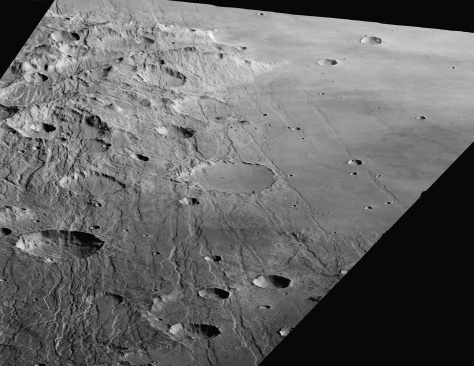
\includegraphics[height=4cm,keepaspectratio]{images/Gre13_04.jpg}
		\captionsetup{format=plain}
		\subcaption{Beispiel für mehrere Gräben}
		\label{fig:ex_graben}
	\end{subfigure}
	\hfill
	\begin{subfigure}[t]{0.3\textwidth}
		\centering
		\includegraphics[height=4cm,keepaspectratio]{images/Gre13_05.jpg}
		\captionsetup{format=plain}
		\subcaption{Beispiel für einen Gletscher}
		\label{fig:ex_glacier}
	\end{subfigure}
	\hfill
	\begin{subfigure}[t]{0.25\textwidth}
		\hfill
	\end{subfigure}
	\caption{Beispiele für Merkmale der Marsoberfläche, alle aus \cite[Kap.~7]{greeley_13}}
\end{figure}

Die wohl signifikantesten Merkmale der Oberfläche sind \ua: \cite[Kap.~7]{greeley_13}
\begin{itemize}
	\item Einschlagskrater:\\
Einschlagskrater können sich stark in der Größe unterscheiden: So haben die größten Exemplare einen Durchmesser von bis zu \SI{1800}{\kilo\meter}, während auch eine Großzahl an sub-\si{\kilo\meter} Kratern existieren. Diese Eigenschaft erschwert die zuverlässige Erkennung erheblich, da die angewandte Methode in der Lage sein muss, die zur Erkennung genutzen Merkmale stark in der Größe zu variieren. Es existieren zwar verschiedene Variationen, die meisten Krater gleichen aber einfachen kreisförmigen Vertiefungen, wie in \figurename~\ref{fig:ex_crater} dargestellt.
	\item Vulkanartige Merkmale:\\
Merh als die Häfte der Marsoberfläche ist von Vulkanen bedeckt. \cite[Kap.~7]{greeley_13} Es existieren verschiedene Arten von Vulkanen mit jeweils verschiedenen Merkmalsausprägungen. Einige der häufigsten Merkmale sind eine kuppelartige Form (\vgl \figurename~\ref{fig:ex_vulc1}) und sich strahlenförmig ausbreitende Schluchten, ausgelöst durch den früheren Lava-Fluss (\vgl \figurename~\ref{fig:ex_vulc2}). \cite[Kap.~7]{greeley_13}
	\item Tektonische Merkmale:\\
Tektonische Veränderungen der Marsoberläche können verschiedene Ursachen haben, wie \zB das Auftreten von Vulkanen, Einschlägen oder anderen Verformungen der Litosphäre. \cite[Kap.~7]{greeley_13} Hierbei wird oft zwischen ausdehnenden und komprimierenden tektonischen Veränderungen unterschieden. Während ausdehnende Veränderungen zu Schluchten \bzw Gräben führen (\vgl \figurename~\ref{fig:ex_graben}), werden durch die Komprimierung Hügelketten erschaffen.
	\item Oberflächenbeschaffenheit:
Auch ohne Einwirkungen von Kratern, Vulkanen, \etc weißt die Marsoberfläche unterschiedliche Beschaffenheiten auf. So sind -- insbesondere an den Polen -- oft Gletscher zu finden (\vgl \figurename~\ref{fig:ex_glacier}). Des Weiteren kann sich diese Beschaffenheit auch durch Erosionen verändern \bzw verändert haben, sowohl durch Wind als auch durch Wasser.
\end{itemize}

Diese Faktoren sorgen für eine große Varietät an optisch unterschiedlichen Oberflächen des Mars. Erkennbar sind sie auf Fotografien nur durch das flach einfallende Licht, welches Erhebungen und Täler durch Schatten und Highlights sichtbar macht. Durch diesen Effekt werden auch die unterschiedlichen, zu analysierenden Texturen erkennbar.

\subsection{Remote Sensing Instruments}
\label{ssec:mars_images}

Von der Marsoberfläche existieren verschiedenste Arten von Aufnahmen für unterschiedliche Analysen. Dabei sind gewisse Parameter, wie \zB die aufgenommene Wellenlänge, den Winkel zur Oberfläche, die Auflösung, Brennweite, Ort der Aufnahme und viele weitere wichtig, damit ein Bild zur Analyse einer gewissen Eigenschaft geeignet ist.

Für die hier genutzten Anwendungsfälle eignen sich Instrumente gut, die sichtbares Licht aufnehmen. Obwohl Farbaufnahmen in vielerlei Hinsicht von Vorteil zur Analyse wären, sind diese nicht großflächig vorhanden, daher werden Graustufenaufnahmen als Kompromiss benutzt. Diese besitzen den Vorteil, dass nur ein drittel des Speichers bei den Berechnungen benötigt wird, da statt separaten Rot-, Grün- und Blauwerten nur ein Helligkeitswert gespeichert und verarbeitet werden muss.

Des Weiteren sollten die Bilder eine vergleichsweise hohe Auflösung haben, damit auch kleinere Merkmale gut erkannt werden können. Dies stellt einen Konflikt mit einer weiteren Anforderung dar, da ein Datensatz gesucht wird, der einen Großteil der Oberfläche abdeckt.

Außerdem eignen sich Aufnahmen gut, die senkrecht zur Oberfläche entstanden sind, so dass Objekte auf dieser möglichst denselben Maßstab besitzen.

Unter Berücksichtigung dieser Faktoren ergeben sich \ua zwei geeignete Instrumente:
Die \textit{Context Camera (CTX)} des \textit{Mars Reconnaissance Orbiters} der NASA \cite{malin_07} und die \textit{High Resolution Stereo Camera (HRSC)} des \textit{Mars Express Orbiters} der ESA \cite{hrsc}. Für die eigentlichen Analysen werden Aufnahmen der CTX genutzt, da sie einen Großteil der Oberfläche abdecken.%, während die panchromatischen Bilder der HRSC zur Evaluierung genutzt wurden, da mit ihnen schon mehrere andere Algorithmen getestet wurden.

\section{Convolutional Neural Networks}
\label{sec:cnn}

Neuronale Netze werden oftmals als eine Weiterentwicklung oder Optimierung des maschinellen Lernens betrachtet: Statt einer Menge von (Differential)gleichungssystemen, welche die Approximation einer Funktion erlernen sollen und \ggf für den jeweiligen Anwendungsbereich angepasst werden müssen, setzt man bei neuronalen Netzen auf mehrere Schichten, auch Layers genannt, von vergleichsweise einfachen linearen Funktionen um zur gewünschten Approximation zu kommen. \cite{hardesty_17}

Eine der einfachsten Formen eines neuronalen Netzes besteht aus dem Multilayer-Perceptron: Dieses besteht aus mehreren der zuvor erwähnten Layers, von denen jede mehrere einzelne Perceptronen enthält. Zwischen einer Eingabe- und einer Ausgabe-Schicht existieren somit auch noch eine beliebige Anzahl an sogenannten Hidden Layers.

In diesem Kontext wird ein Perceptron auch als Neuron bezeichnet. Ein typisches Neuron verarbeitet einen Eingabevektor indem es dies mit einem Gewichtungs-Vektor elementweise multipliziert und anschließend einen Bias-Vektor aufaddiert. Die Addition dieses Bias ist nötig um die gesamte Aktivierungsfunktion entlang der x-Achse verschieben zu können, da sonst manche gewünschten Ergebnisse nicht erreicht werden können. \cite{bias} Ein typisches Neuron ist in \figurename~\ref{fig:neuron} dargestellt. Anschließend werden die Elemente dieses Vektor aufaddiert, und auf diese Summe eine Aktivierungsfunktion (\vgl Unterabschnitt~\ref{ssec:activation}) angewandt. Während das Netzwerk trainiert wird, passen die einzelnen Perceptronen diese zwei Vektoren, also die Gewichtungen und die Bias, so an, dass die Ergebnisse weitgehend optimiert werden (\vgl Unterabschnitt~\ref{ssec:backpropagation}). Diese Gewichtungen sind anfangs zufällig bestimmt. \cite{hardesty_17, cs231n} 

\begin{figure}[h!]
	\centering
	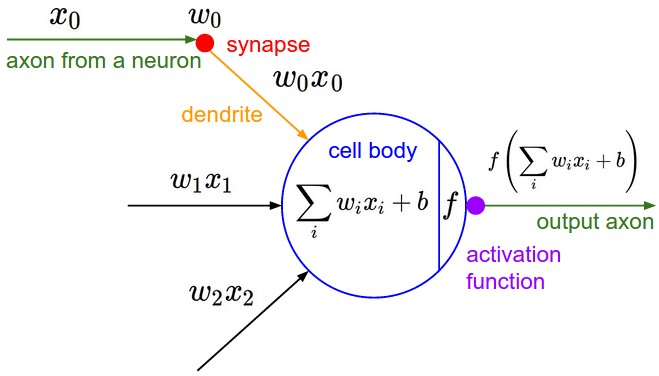
\includegraphics[width=0.5\textwidth,keepaspectratio]{images/cs231n/neuron.jpg}
	\caption{Funktionsweise eines Neurons, aus \cite{cs231n}}
	\label{fig:neuron}
\end{figure}

Die Aneinanderkettung dieser Schichten führt dazu, dass zwischen ihnen eine immer abstraktere Form der Eingabedaten entsteht.

Convolutional Neural Networks beschreiben eine Teilmenge der neuronalen Netze, in der die jeweilige Netzwerkarchitektur mindestens eine Convolutional Layer (auch Faltungsschicht genannt, \vgl Unterabschnitt~\ref{ssec:conv}) enthält. Die Nutzung dieser Convolutional Layer zieht oft die Nutzung einer Pooling Layer (Unterabschnitt~\ref{ssec:pooling}) mit sich. \cite{deeplearning_16}

Obwohl Convolutional Neural Networks theoretisch dazu geeignet sind die meisten Daten mit einer gitterähnlichen Struktur zu verarbeiten, erfreuen sie sich im Bereich der Bilddatenanalyse der größten Beliebtheit. \cite[Kap.~9]{deeplearning_16} Eine wichtige Ursache für diese Beliebtheit liegt \bspw in dem Erfolg bei dem Bild-Klassifizierungs-Wettbewerb \textit{ImageNet}. Während dort im Jahr 2011 die Gewinnergruppe mit klassischen Klassifizierungsalgorithmen einen Top-5-Score von $74,3\%$ erzielt hat, wurden im Jahr 2012 mit einem CNN (AlexNet, \cite{alexnet}) erstmals ein Wert von $83,6\%$ erreicht. Von diesem Punkt an wurde die Bestenliste der darauffolgenden Jahre durch Convolutional Neural Networks dominiert. \cite[Kap.~1]{deeplearning_18}

Neben der genannten Objekterkennung eigenen sie sich auch zur Bildsegmentierung. So werden sie \bspw erfolgreich in der Entwicklung von selbstfahrenden Autos eingesetzt. \cite{kaymak_19}

Die Architektur eines typischen, einfachen Convolutional Neural Networks ist wie folgt \cite{cs231n}:

\begin{multline*}
\mathrm{INPUT}\rightarrow\mathrm{CONVOLUTIONAL}\rightarrow\mathrm{ACTIVATION}\\\rightarrow\mathrm{POOLING}\rightarrow\mathrm{FULLYCONNECTED}
\end{multline*}

Da CNNs primär auf Bilddateien angewandt werden, wird von diesem Punkt an von einer Bilddatei als Eingabe ($\mathrm{INPUT}$) ausgegangen. Hier beschreiben die ersten beiden Dimensionen die Breite und Höhe, während die dritte Dimension die Farbwerte für den jeweiligen Pixel angibt. Die Konvolutions-, Aktivierungs-, Pooling- und Fully-Connected-Layers werden in den folgenden Unterabschnitten erläutert.

\subsection{Konvolution}
\label{ssec:conv}

\noindent In den kommenden Formeln werden die folgenden Variablen genutzt:
\begin{description}
\item  $f(x)$, $g(y)$: Beliebige Funktionen mit den jeweiligen Parametern $x$ und $y$
\item  $s(x)$: Konvolution der Funktionen $f(x)$ und $g(y)$\\
\end{description}
\noindent \Bzw in praktischer Anwendung:
\begin{description}
\item  $x(t)$: Eine Reihe von Messwerten in Abhängigkeit des Zeitpunktes ihrer Messung
\item  $w(a)$: Eine Gewichtungsfunktion in Abhängigkeit des Alters der Messung (\iA Kernel genannt)
\end{description}

\bigskip

Die Konvolution ist eine mathematische Operation auf zwei Funktionen $f(x)$ und $g(y)$, die eine dritte Funktion, die Konvolution $s = f*g$ ergibt, welche beschreibt, wie sich die Verläufe der beiden Funktionen beeinflussen:

\begin{equation}
s(x) = (f*g)(x) = \int_{-\infty}^{\infty} f(y)g(x-y)dy
\end{equation}

In einem Großteil der Anwendungsfälle der Konvolution bestehen die Eingabefunktionen aus einer Eingabefunktion $x$ und einem Kernel $w$, die Ausgabe ist die Merkmalsdimension. In einer praktischen Anwendung wären dies \bspw Messwerte $x(t)$ in Abhängig von der Zeit und einer Gewichtungsfunktion $w(a)$ in Abhängigkeit des Alters der Messung. Für ungültige Zeiten (\bspw Messwerte welche sich in der Zukunft befinden würden) gilt $w=0$ \cite[Kap.~9]{deeplearning_16}:

\begin{equation}
s(t) = (x*w)(t) = \int_{-\infty}^{\infty} x(a)w(t-a)da
\end{equation}

Unter der Annahme, dass die Eingabewerte nicht stetig sondern diskret sind (\bspw zeitliche Messwerte in regelmäßigen Abständen) ergibt sich vereinfacht \cite[Kap.~9]{deeplearning_16}:

\begin{equation}
s(t) = (x*w)(t) = \sum_{a=-\infty}^{\infty}x(a)w(t-a)
\end{equation}

Diese Funktion lässt sich für zweidimensionale Eingabedaten, wie \zB eine Bilddatei $I$ und einen zweidimensionalen Kernel $K$ erweitern \cite[Kap.~9]{deeplearning_16}:

\begin{equation}
S(i,j) = (I*K)(i,j) = \sum_{m}\sum_{n}I(m,n)K(i-m,j-n)
\end{equation}

Eine alternative Betrachtungsweise dieser Formel basiert auf dem Hadamard-Produkt. Angenommen, es existieren eine Matrix $I\in\mathbb{R}^{2}$ und eine Matrix $K\in\mathbb{R}^{m\times n}$.

Sei Matrix $H$ definiert als Hadamard-Produkt aus $K$ und $I'=I_{x, y}$ mit $x\in[i-m,i]$ und $y\in[j-n,j]$.\\
Dann gilt: $S(i,j)=(I*K)(i,j) = \sum_{m}\sum_{n}I(m,n)K(i-m,j-n)=\sum_{h\in H}h$

Diese Formel ist allerdings nur für Eingabebilder mit nur einem Farbwert pro Pixel gültig, also Graustufenbilder. Für ein Bild mit beliebig vielen Farbwertsdimensionen gilt:

\begin{equation}
S(i,j) = (I*K)(i,j) = \sum_{m}\sum_{n}\sum_{o}I(m,n,o)K(i-m,j-n,o)
\end{equation}

Es ist zu beachten, dass der Farbvektor immer komplett verarbeitet wird, und nicht nur ein Teilausschnitt wie bei Höhe und Breite.

\subsection{Convolutional Layer}
\label{ssec:convlayer}

Klassische Schichten von neuronalen Netzen nutzen Matrixmultiplikationen der kompletten Eingabe mit einer Parametermatrix um ihre Ausgaben zu berechnen, \dahe jeder einzelne Ausgabewert entsteht aus einer Berechnung basierend auf jedem einzelnen Eingabewert. Obwohl diese Taktik in vielen Einsatzbereichen gut funktioniert, stößt sie insbesondere bei der Bilddatenanalyse an ihre Grenzen, da sie nicht gut skaliert. \cite{cs231n} So benötigt eine Convolutional Layer zum Erkennen eines Merkmals nur einen Kernel mit einer Anzahl von meistens unter $\SI{100}{\pixel}$. \cite{deeplearning_16} Ein weiterer Pluspunkt besteht daraus, dass durch Convolutional Layers bestimmte Merkmale von unterschiedlichen Stellen der Eingabe extrahiert werden können, wie später beschrieben.

\begin{figure}[H]
	\centering
	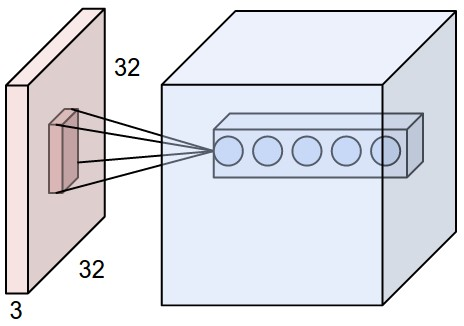
\includegraphics[width=0.4\textwidth,keepaspectratio]{images/cs231n/convolutional.jpg}
	\caption{Funktionsweise der Konvolutions-Schicht, aus \cite{cs231n}}
	\label{fig:convolutional}
\end{figure}

Eine konvolutionelle Schicht besteht aus einer Menge von Neuronen, welche die Eingabe über den eben beschriebenen Konvolutionsoperator $S(i,j)$ auf genau ein Merkmal untersuchen. Daraus folgt, dass die Anzahl der Neuronen in eben dieser Schicht gleich der Größe der entstehenden Merkmalsdimension ist. (\vgl \figurename~\ref{fig:convolutional})

Das Hinzufügen von konvolutionellen Schichten führt allerdings zu mehr Hyperparametern, die optimiert werden können \cite{cs231n}:
\begin{itemize}
	\item Die Dimensionen des Kernels $k_1$ und $k_2$ (obwohl dieser fast immer quadratisch ist, oftmals $3$)
	\item Die Anzahl der Neuronen/der Merkmalsdimensionen
	\item Die Größe der Strides (die Schrittweite). Hier wird von einem Wert von $1$ ausgegangen, was die Größe der Ausgabe nicht verändert.
	\item Das Padding, also wie sich die Konvolution an den Rändern der Eingabedaten verhält. Hier wird von Zero-Padding ausgegangen, \dahe dass außerhalb der Ränder der Eingabe alle Werte gleich Null sind. Dies hat zur Folge, dass es die Größe der Ausgabe unverändert lässt.
\end{itemize}

Es gilt es zu beachten, dass der Konvolutionsoperator für alle Werte $i$ und $j$ der Eingabedimensionen aufgerufen wird, so dass die Höhe und Breite der Ausgabe (bis auf einige Ausnahmen) identisch zu denen der Eingabe ist.
Des Weiteren ist der Kernel pro Neuron konstant. Dies hat \ua zur Folge, dass das gleiche Merkmal an verschiedenen Stelle in der Eingabe erkennen kann.

Erhält eine konvolutionelle Schicht mit 12 Neuronen also \bspw ein RGB-Eingabebild der Größe $\SI{64}{\pixel}\times\SI{64}{\pixel}$, so erzeugt es mit einem Stride von $1$ als Ausgabe eine dreidimensionale Matrix der Größe $64\times64\times12$, jede der Schichten der dritten Dimensionen deutet auf das Vorhandensein eines speziellen Merkmals an einer gewissen Stelle im Eingabebild hin.

\subsection{Activation Layer}
\label{ssec:activation}

Auf eine konvolutionelle Schicht folgt fast immer eine Aktivierungsschicht. Diese werden dazu genutzt um eine gewisse Nicht-Linearität in den Verlauf des neuronalen Netzes einzuführen. Nicht-Linearität ist in vielen neuronalen Netzen notwendig, da die Probleme, die sie lössen sollen, nicht-linear sind. \cite[Kap.~6]{deeplearning_16}

Selbst wenn nach der letzten Schicht eines mehrschichtigen neuronalen Netzes eine Aktivierungsschicht hinzugefügt werden würde, hätte dies zur Folge, dass die vorherigen Schichten wie eine einzige lineare Schicht agieren, was keine Vorteile gegenüber einer einzigen Schicht hat. Somit sollte auf jede einzelne Schicht eine Aktivierungsschicht folgen, um verschiedenste, komplizierte Zusammenhänge zwischen Ein- und Ausgabedaten besser approximieren zu können. \cite[Kap.~3]{deeplearning_18}

In \figurename~\ref{fig:activations} sind drei der am meisten Verbreiteten Aktivierungsfunktionen zu sehen.

\begin{figure}[h!]
	\begin{subfigure}{0.33\textwidth}
		\centering
		\begin{tikzpicture}[scale=0.6]
			\begin{axis}[
				axis lines = middle,
				xlabel = {$x$},
				ylabel = {$f(x)$},
				domain=-5:5,
				]
				\addplot[draw=blue,samples=100,domain=-5:5,line width=1.5]{max(0,x)};
				\addplot[draw opacity=0,domain=-5:5]{1.2*x};
			\end{axis}
		\end{tikzpicture}
		\subcaption{ReLU:\\$f(x)=\mathrm{max}\{0,x\}$}
		\label{fig:relu}
	\end{subfigure}
	\begin{subfigure}{0.32\textwidth}
		\centering
		\begin{tikzpicture}[scale=0.6]
			\begin{axis}[
				axis lines = middle,
				xlabel = {$x$},
				ylabel = {$f(x)$},
				domain=-5:5,
				]
				\addplot[draw=blue,samples=100,domain=-5:5,line width=1.5]{1/(1+e^(-x))};
				\addplot[draw opacity=0,domain=-5:5]{0.3*x};
			\end{axis}
		\end{tikzpicture}
		\subcaption{Sigmoid:\\$f(x)={1}/{(1+e^{-x})}$}
		\label{fig:sigmoid}
	\end{subfigure}
	\begin{subfigure}{0.33\textwidth}
		\centering
		\begin{tikzpicture}[scale=0.6]
			\begin{axis}[
				axis lines = middle,
				xlabel = {$x$},
				ylabel = {$f(x)$},
				domain=-5:5,
				]
				\addplot[draw=blue,samples=100,domain=-5:5,line width=1.5]{tanh(x)};
				\addplot[draw opacity=0,domain=-5:5]{0.3*x};
			\end{axis}
		\end{tikzpicture}
		\subcaption{tanh:\\$f(x)=tanh(x)$}
		\label{fig:tanh}
	\end{subfigure}
	\caption{Drei Aktivierungsfunktionen}
	\label{fig:activations}
\end{figure}

Die intuitivste Aktivierungsfunktion, die Einheitssprungfunktion, wird in neuronalen Netzen nur für Binärklassifizierungsprobleme in der letzten Schicht genutzt. Dies rührt daher, dass sie keine Ableitung besitzt und daher nicht zum Lernen über Backpropagation (\vgl Unterabschnitt~\ref{ssec:backpropagation}) geeignet ist.

Die ReLU-Aktivierungsfunktion (\vgl \figurename~\ref{fig:relu}) ist die wohl einfachste (nicht-lineare) Funktion, die als Aktivierungsfunktion geeignet ist. Diese Einfachheit führt zu einer vergleichsweise guten Performance, und deshalb großer Beliebheit in neuronalen Netzen mit vielen Schichten. Ihr Nachteil besteht darin, dass für Bereich $x<0$, praktisch gesehen kein Lernprozess stattfindet, da sie dort immer $0$ beträgt. \cite{kizrak_19}

Die Sigmoid-Funktion eignet sich gut als Aktivierungsfunktion, da sie im Bereich nahe der y-Achse eine hohe Steigung aufweist, während die Veränderungen in anderen Bereichen relativ klein ausfallen. Damit eignet sie sich gut zur Klassifizierung. \cite{kizrak_19}

Die $tanh(x)$-Funktion ist in ihrer Rolle als Aktivierungsfunktion relativ ähnlich zur Sigmoid-Funktion, mit dem Unterschied dass sie im negativen x-Bereich auch ins Negative geht, statt sich an $0$ anzunähern. Wie die Sigmoid-Funktion eignet sie sich gut zur Klassifizierung, je nach Anwendungsfall sogar besser, da ihre Ableitung nahe der y-Achse steiler ist. \cite{kizrak_19}

Es existieren noch weitere Aktivierungsfunktionen, diese zu Analysieren ist allerdings außerhalb des Rahmens dieser Arbeit.

\subsection{Pooling Layer}
\label{ssec:pooling}

Konvolutionelle Schichten in neuronalen Netzen können die selben Merkmale von unterschiedlichen Stellen extrahieren. Die Position, an der diese Merkmale erkannt wurden, werden auch an die nächste Schicht weitergegeben, \dahe kleine Veränderungen an der Position eines Merkmals führen zu einer veränderten Merkmalsdimension. \cite{brownlee_19} Dies kann insbesondere beim Einsatz von mehreren konsekutiven Convolutional Layers zu einer erhöhten Störanfälligkeit führen, deshalb wird oftmals eine Pooling-Layer dazu eingesetzt, das resultierende Netzwerk invariant zu einzelnen Merkmalspositionen zu machen. Des Weiteren dient eine Pooling-Layer dazu, Informationen aus verschiedenen Bildbereichen zu abstrahieren und langsam global zu aggregieren. \cite{deeplearning_16}

\begin{figure}[h!]
	\centering
	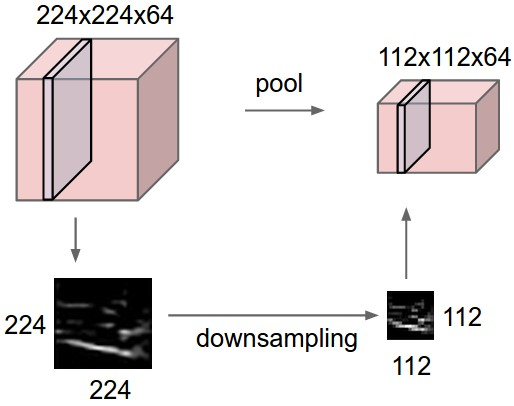
\includegraphics[width=0.37\textwidth,keepaspectratio]{images/cs231n/pool.jpg}
	\caption{Funktionsweise der Pooling-Layer, aus \cite{cs231n}}
	\label{fig:pooling}
\end{figure}

Ein weiteres Problem des Einsatzes von ausschließlich konvolutionellen Schichten besteht daraus, dass sie schnell zu einem hohen Anstieg der Parameterzahl im Netzwerk führen können: Jede neue Schicht erzeugt einen weiteren Datenwürfel der Größe $H\times W\times F$, wobei $H$ und $W$ die Höhe und Breite des Eingabebildes, und $F$ die Größe der Merkmalsdimension ist. Alle diese Werte werden im Training des neuronalen Netzes optimiert, was zu Performanceeinbüßungen führen kann. \cite{cs231n}

Die Pooling-Schicht verarbeitet alle Merkmalsdimensionen ihrer Eingabe unabhängig voneinander.

Für jede Merkmalsdimension überlauft der rezeptive Bereich -- ähnlich zur Konvolutions-Schicht -- die jeweilige Schicht des Würfels in Höhe und Breite, und berechnet je nach Pooling-Art einen Wert, welcher als positionsabhängige Ausgabe weitergeleitet wird. Dieser Prozess ist in \figurename~\ref{fig:pooling} anschaulich dargestellt.

Er besitzt zwei Hyperparameter: Die Stride (Schrittweite) $S$ und die eigentliche Größe $F_1\times F_2$. \cite{cs231n}

\begin{figure}[H]
	\centering
	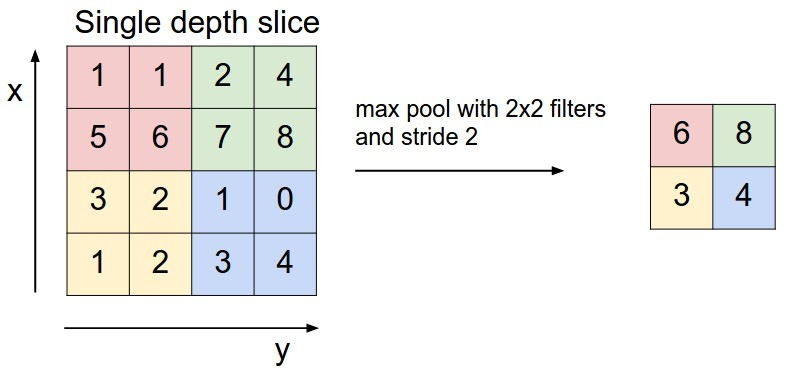
\includegraphics[width=0.6\textwidth,keepaspectratio]{images/cs231n/maxpool.jpg}
	\captionsetup{width=0.6\textwidth}
	\caption{Max-Pooling anhand eines Beispiels, aus \cite{cs231n}}
	\label{fig:maxpooling}
\end{figure}

Beim Max-Pooling übernimmt die Poolingoperation den maximalen Wert des von ihr überdeckten Eingabebereiches. (\vgl \figurename~\ref{fig:maxpooling})

\subsection{Fully Connected Layer}
\label{ssec:fcn}
Die meisten Convolutional Neural Networks besitzen eine Fully Connected Layer. Das Ziel dieser besteht daraus, die Resultate der konvolutionellen und Pooling-Schichten zu klassifizieren, da diese nur die Wahrscheinlichkeiten zurückgeben, mit der ein gewisses Merkmal an einer gewissen Position erkannt wird. Aus diesem Grund werden eine oder mehrere Fully Connected Layers am Ende eines ansonsten fertigen neuronalen Netzes eingesetzt. \cite{geva}

Die Funktionsweise einer Fully Connected Layer ist identisch zu einer Schicht eines Multilaye-Perceptrons, wie in Abschnitt~\ref{sec:cnn} beschrieben.

\subsection{Batch Normalization}
\label{ssec:bn}

\subsection{Loss Function}
\label{ssec:loss}

Das Ziel eines neuronalen Netzes ist es, den Loss in jeder Iteration weiter zu minimieren. Der Loss, auch Verlustfunktion genannt beschreibt, wie stark sich die vom Netz berechneten Werte von den zu erzielenden Werten (beim überwachten Lernen meistens die Ground Truth) unterscheiden.

Auch hier existieren verschiedenste Loss-Funktionen. Im Folgenden wird genauer auf den Cross-Entropy-Loss eingegangen. Dieser ist besonders für Klassifizierungsprobleme geeignet. Er ist definiert als \cite{cs231n}:

\begin{equation}
H(p,q) = -\sum_x p(x)\log q(x)
\end{equation}

Dabei gibt $p$ die korrekten Klassen als one-hot-kodierter Vektor an: $p$ ist also ein Vektor mit $n$ Elementen, wobei $n$ die Anzahl der möglichen Klassen ist. 

Es gilt: $f_i$ ist gleich dem $i$-ten Element eines Eingabevektors $f$.

Eine korrekte Klasse wird mit einer $1$ am entsprechenden Element im Vektor kodiert, alle anderen Felder sind gleich $0$. Ist für die jeweilige Eingabe nun \bspw die $m$-te Klasse korrekt, so gilt $p_m=1$ und $p_{\left[1,m-1\right]} = p_{\left[m+1,n\right]} = 0$. Es ist zu beachten, dass der Cross-Entropy-Loss ausschließlich die Wahrscheinlichkeiten für korrekte Klassen bewertet.

$q$ hingegen gibt die berechnete Wahrscheinlichkeit an, dass eine jeweilige Klasse auf die Eingabe zutrifft. Da für $q$ eine Wahrscheinlichkeit im Intervall $[0,1]$ benötigt wird, wird als dessen Eingabe meistens die Softmax-Funktion der vorhergehenden Werte genutzt. Die Softmax-Funktion kann wie die ReLU- oder die Sigmoid-Funktion als Aktivierungsfunktion betrachtet werden. Sie ist definiert durch \cite{cs231n}:

% TODO Warum softmax als Aktivierung?
\bigskip
{ TODO WARUM WIRD SOFTMAX GENUTZT}
\bigskip

\begin{equation}
S_i=\dfrac{e^{f_i}}{\sum_j e^{f_j}}
\end{equation}

Kombiniert ergibt sich so also für den Cross-Entropy-Loss \cite{cs231n}:

\begin{equation}
L_i = -\sum_x p(x)\log\left(\dfrac{e^{f_{y_i}}}{\sum_j e^{f_i}}\right)
\end{equation}

Da für alle außer eine Klasse gilt $p=0$, lässt sich die Summe entfernen:

\begin{equation}
L_i = -\log\left(\dfrac{e^{f_{y_i}}}{\sum_j e^{f_i}}\right)
\end{equation}


Für den durchschnittlichen Loss über alle Klassifizierungen ergibt sich so:

\begin{equation}
L = \dfrac{1}{N}\sum_{i=1}^{N}L_i
\end{equation}

Hier ist allerdings zu beachten, dass es für ein neuronale Netz mehrere optimale Gewichtungen und Bias geben kann: Würde man \bspw alle Gewichtungen mit dem selben Skalar multiplizieren, würden diese immer noch zu dem selben Ergebnis führen. Um möglichst kleine Gewichtungen und Biase zu bestimmen, wird ein Regularisierungsterm eingeführt um die Gewichtungen möglichst gering zu halten \cite{cs231n}:

\begin{equation}
L = \dfrac{1}{N}\sum_{i=1}^{N}L_i + \lambda R(W)
\end{equation}

mit $\lambda$ als einem Hyperparameter zur Gewichtung und

\begin{equation}
R(W) = \sum_k\sum_l W^2_{k,l}
\end{equation}

\subsection{Gradientenverfahren}
\label{ssec:gradientenverfahren}

Das Ziel eines neuronalen Netzes besteht daraus, die Werte der Lossfunktionen weitgehend zu minimieren. Dies wäre rein theoretisch durch klassische Analysis möglich, indem man die Ableitungen der Funktionen Netzes berechnet und aus diesen anschließend die Extrempunkte. In der Praxis allerdings, besitzt so ein Netzwerk viel zu viele Variablen, als dass die Extremalstellen in einem Annehmbaren Zeitraum berechnet werden könnten. \cite[Kap.~1]{nielsen_15} AlexNet, der Gewinner der ImageNet-Challenge 2012 besitzt \bspw etwa 60 Millionen trainierbare Parameter. (\Vgl Abschnitt~\ref{sec:cnn})

Die Funktion $C(w, b)$ sei die zu minimierende Lossfunktion in Abhängigkeit von den Gewichtungen und Bias des neuronalen Netzes. Zur einfacheren Erklärung gilt, \oBdA, dass im Netzwerk nur zwei trainierbare Parameter existieren. Somit ist das Ziel, die Parameter der Funktion $C(v_1, v_2)$ so zu optimieren, dass das Funktionsergebnis minimiert wird. Grafisch ist eine Beispielfunktion $C$ in \figurename~\ref{fig:valley} dargestellt.

\begin{figure}[h!]
	\centering
	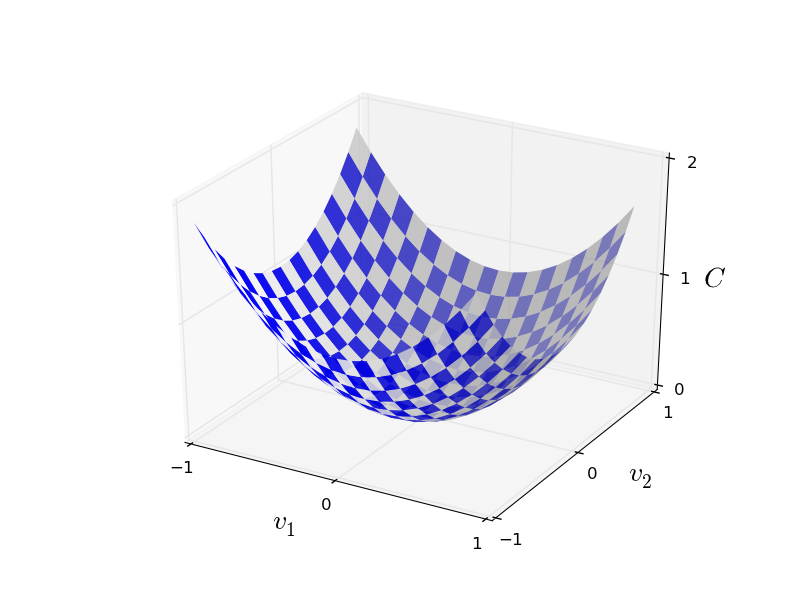
\includegraphics[width=0.45\textwidth,keepaspectratio]{images/Nie15_01.png}
	\caption{Funktion $C$ in Abhängigkeit von $v_1$ und $v_2$, aus \cite{nielsen_15}}
	\label{fig:valley}
\end{figure}

Das Gradientenverfahren beschreibt einen Prozess zur Lösung dieses Problems: Bei diesem Verfahren beginnt man bei einem Startpunkt auf dem Funktionsgraphen. Von dort aus wird ermittelt, in welche Richtung der Graph (hier) absteigend verläuft. Man schreitet nun in diese Richtung und wiederholt das Verfahren. Dies geschieht so lange, bis man an einem Punkt angelangt, von welchem aus es in keine Richtung mehr bergab geht. Dieser Punkt ist ein lokales Minimum. Es gilt zu beachten, dass die Weite des jeweiligen Schrittes variabel ist: Es kann somit geschehen, dass am Ende des Verfahrens, der jeweilige Punkt um das lokale Minimum herum schwankt.

\subsection{Backpropagation}
\label{sec:backpropagation}

\chapter{Verwandte Arbeiten}
\label{chap:related}

Da in dieser Arbeit verschiedene Forschungsbereiche miteinander kombiniert werden, ist dieses Kapitel in zwei Abschnitte eingeteilt: Es wird mit einigen verwandten Arbeiten im Bereich der Bildsegmentierung begonnen, dabei wird insbesondere auf die Nutzung von neuronalen Netzen eingegangen. Anschließend werden Clusteringprozesse betrachtet, welche zur Initialisierung der Segmentierungsalgorithmen genutzt werden. 

Zuletzt folgt die Analyse der Marsoberfläche, insbesondere der Kratererkennung.
% TODO Remove mars?

\section{Bildsegmentierung}
\label{sec:image_segmentation}

\subsection{DEC -- Deep Embedded Clustering}
\label{ssec:dec}
In \cite{junyuan_16} wird eine Methode zur Bildsegmentierung durch neuronale Netze ohne vorherige Ground Truth vorgestellt: Das Ziel besteht daraus, $N$ Punkte $\{x_n\in X\}_{n=1}^N$ in $k$ verschiedene Cluster mit den jeweiligen Clusterzentren $\mu_j, j\in\left[1, k\right]$ einzuteilen. Entgegen des naiven Ansatzes, direkt die Farbwerte der einzelnen Pixel als Merkmalsraum $X$ zu nutzen und zu clustern, wird in \cite{junyuan_16} nicht direkt anhand der Farbwerte geclustert, stattdessen wird dieser zuerst über eine nichtlineare Funktion $f_\theta: X\rightarrow Z$ in einen Merkmalsraum $Z$ abgebildet. $\theta$ ist dabei ein erlernbarer Parameter, sodass das genutzte Neuronale Netz zwei Parameter zeitgleich optimiert: $\theta$, und die Position der Clustermitten $\mu_j$.

Der DEC-Algorithmus besteht aus zwei Phasen:
\begin{enumerate}
	\item{Parameterinitialisierung:}\\
	Um die Startparameter für $\theta$ zu Generieren wird ein Stacked Autoencoder (SAE, \cite{vincent_10}) schichtenweise aufgebaut. Jede Schicht des SAEs ist ein rauschunterdrückender Autoencoder, welcher wie folgt definiert ist: \cite{junyuan_16}
	\begin{eqnarray}
	\bar{x}&\sim&Dropout(x)\\
	h &=& g_1(W_1\tilde{x}+b_1)\\
	\tilde{h} &\sim& Dropout(h)\\
	y &=& g_2(W_2\tilde{h}+b_2)
	\end{eqnarray}
	Zuerst wird ein Encoder-Decoder-Paar dazu trainiert, ein Signal wiederherzustellen, nachdem dieses eine Encoder-Schicht durchlaufen hat. Anschließend wird der Parameter $h$ dazu genutzt, ein weiteres Paar zu trainieren (\vgl \figurename~\ref{fig:sae}). Am Ende dieses Lernens besteht $\theta$ aus der Menge aller Gewichtungen $W$ und Bias $b$ der verschiedenen Encoder Schichten. Diese Encoder-Schichten beschreiben nun die Funktion $f_\theta$, welche den originalen Merkmalsraum $X$ des Bildes in den reduzierten Merkmalsraum $Z$ umwandelt.
	
	Die initialen Clustermitten werden durch den k-Means-Algorithmus auf dem Merkmalsraum $Z$ generiert.
	
	\item{Parameteroptimierung:}\\
	Das eigentliche Lernen des DEC-Algorithmus findet in zwei, sich gegenseitig abwechselnden Phasen statt:
	
	Zuerst wird eine Zuweisung von den Datenpunkten des Merkmalsraumes zu den Koordinaten der Clusterzentren berechnet. Zu diesem Zweck wird eine Wahrscheinlichkeitsverteilung, die t-Verteilung genutzt:
	
	\begin{equation}
		f(t)=\frac{\Gamma\left(\frac{\nu+1}{2}\right)}{\sqrt{\nu\pi}\Gamma\left(\frac{\nu}{2}\right)}\left(1+\frac{t^2}{\nu}\right)^{-\frac{\nu+1}{2}}
	\end{equation}
	
	Dabei ist $\Gamma$ die Gamma-Funktion und $\nu$ die Anzahl der Freiheitsgrade.
	
	Diese Funktion berechnet also die Wahrscheinlichkeit, dass ein bestimmter Datenpunkt einem bestimmten Cluster zugewiesen wird.
	
	Anschließend werden die Positionen der Clustermitten $\mu_j$ und die Parameter $\theta$ der Funktion $f_\theta$ optimiert. Die zu verringernde Verlustfunktion ist an dieser Stelle die Kullback-Leibler-Divergenz. Somit wird hier eine Funktion gelernt, welche sich möglichst wenig von der oben beschriebenen, iterativ generierten $t$-Verteilung unterscheidet. Der eigentliche Optimierungsprozess der Clustermitten und der Parameter für $\theta$ findet über das Gradientenverfahren (\vgl Unterabschnitt~\ref{ssec:gradient_descent}) statt.
\end{enumerate}

\begin{figure}[h!]
	\centering
	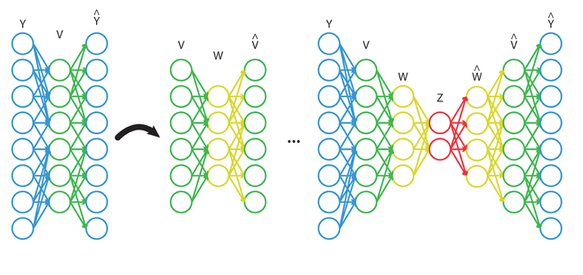
\includegraphics[width=.8\textwidth,keepaspectratio]{images/BK15/BK15_01.png}
	\caption{Initialisierung eines Stacked Autoencoders, modifiziert, aus \cite{berniker_15}. Zu Beginn existiert ein Encoder-Paar (blau) bestehend aus Encoder $Y$ und Decoder $\hat{Y}$ mit einer Zwischenausgabe $V$ (links). Anschließend wird diese Ausgabe $V$ dazu genutzt, ein weiteres Autoencoder-Paar so zu trainieren, dass es die Eingabe $V$ durch $\hat{V}$ approximieren kann (mitte). Dies geschieht iterativ so lange, bis die Anzahl der gewünschten Schichten erreicht ist. Zuletzt werden die so generierten Autoencoder-Paare verschachtelt (rechts).}
	\label{fig:sae}
\end{figure}

Zusammengefasst lernt der Algorithmus in der ersten Phase seiner Ausführung, wie er nach der Anwendung von Dropout-Schichten die ursprüngliche Eingabe bestmöglich wiederherstellen kann, er lernt also wie signifikant bestimmte Merkmale zur Wiederherstellung sind. Diese Initialisierung wird im zweiten Schritt weiter optimiert.
Der Vorteil dieser und ähnlicher Methoden besteht daraus, dass das Netzwerk nicht trainiert werden muss und somit also auch keine Ground Truth benötigt. Dies ermöglicht dessen Einsatz in Bereichen in denen es zu aufwändig ist, Ground Truths manuell zu erstellen. Eine weitere Eigenschaft besteht daraus, dass diese Methode sich für den Einsatz auf unterschiedlichsten Eingabedaten eignet, da sie dynamisch zur Laufzeit lernt, nach welchen Kriterien sie clustern sollte.
% TODO Initialisierung Abbruchkriterium

\subsection{Bildsegmentierung auf Basis eines Bildclusterings}
\label{ssec:kanezaki}
Ein vergleichbarer, wenn auch einfacherer Ansatz wird in \cite{kanezaki_18} beschrieben. Auch dieser Ansatz erstellt eine Mapping-Funktion $c_n=f(x_n)$, die jedem der $N$ $p$-dimensionalen Pixel mit dem Merkmalsvektor $\{x_n\in\mathbb{R}^p\}_{n=1}^N$ eines Eingabebildes ein Clusterlabel $c$ mit $\{c_n\in\mathbb{Z}\}_{n=1}^N$ zuordnet. Anders als beim DEC-Algorithmus wird aber auf Autoencoder verzichtet und zusätzlich direkt im Merkmalsraum der Farbwerte geclustert.

Statt das neuronale Netz selbst eine Initialisierung lernen zu lassen, wird in diesem Algorithmus auf Clusteringalgorithmen aus der Bildverarbeitung zurückgegriffen, insbesondere wird der SLIC-Algorithmus \cite{achanta_10} genutzt.

Eine Segmentierung wird durch einen iterativen Prozess erreicht, in welchem ein anfangs untrainiertes neuronales Netz eine Bildsegmentierung erzeugt, welche anschließend mithilfe der im Vorhinein erstellten, konstanten Segmentierung optimiert wird. Diese Optimierung besteht daraus, dass für jedes Cluster des SLIC-Algorithmus überprüft wird, welches Label das neuronalen Netz am häufigsten den Pixeln im Cluster zugewiesen wurde. Anschließend wird jedes Cluster mit eben diesem häufigsten Label gefüllt und die Differenz zwischen der Ausgabe des Netzwerkes und diesem neu generierten \enquote{Ziel} betrachtet.
Der gesamte Algorithmus ist in \figurename~\ref{fig:Kan18_01} dargestellt, eine genauere Beschreibung findet sich in Abschnitt~\ref{sec:howitworks}.

\begin{figure}[h!]
	\centering
	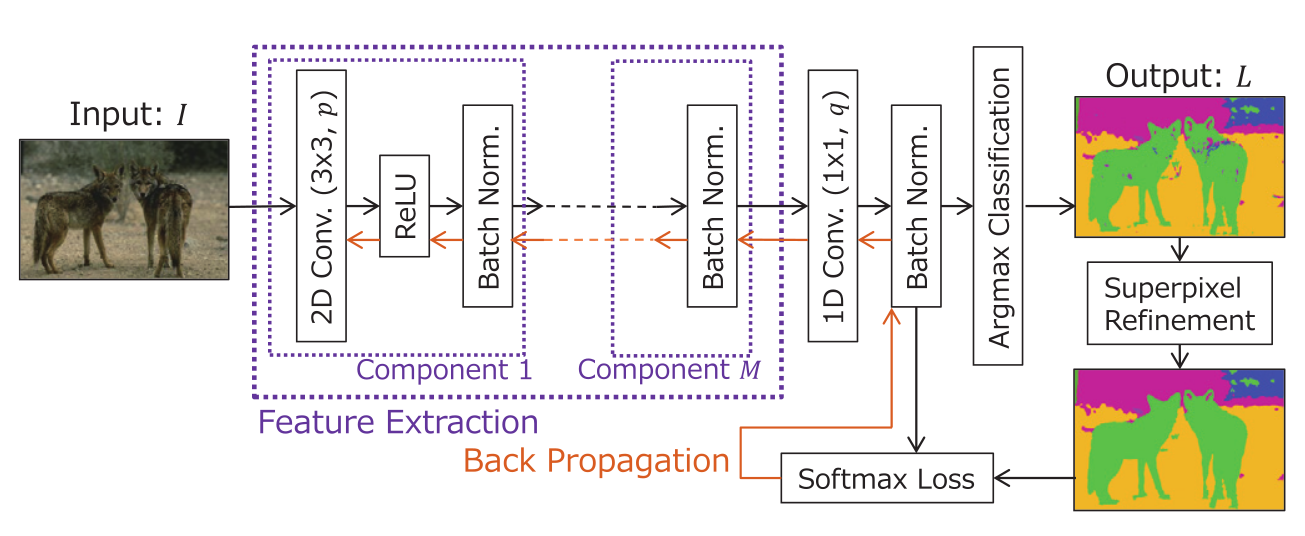
\includegraphics[width=.8\textwidth,keepaspectratio]{images/Kan18/Kan18_01.png}
	\caption{Vorgehensweise nach Kanezaki, aus \cite{kanezaki_18}}
	\label{fig:Kan18_01}
\end{figure}

Es gilt zu beachten, dass zur Initialisierung ein möglichst feines Clustering genutzt wird, da im Laufe des Prozesses mehrere einzelne Cluster miteinander vereint werden, bis die gewünschte Anzahl an Segmenten erreicht wird.

Insgesamt lernt dieser Algorithmus iterativ die Ausgabe der Clusteringfunktion anzunähern, mit dem Unterschied, dass er in diesem Prozess mehrere Clusterzentren miteinander vereinen kann. Da in \cite{kanezaki_18} auf Basis des SLIC-Algorithmus gearbeitet wird, lernt das neuronale Netz hauptsächlich anhand der Farbwerte einzelner Pixel und deren Entfernungen zu ähnlichen Pixeln, wie es eine Eingabe segmentieren soll. Damit kann es als eine vereinfachte Version des DEC-Algorithmus betrachtet werden, da dieser dynamisch bestimmt, Anhand welcher Merkmale das Clustering geschehen soll.

\section{Bildclustering}
\label{ssec:clustering}

Der in Unterabschnitt~\ref{ssec:kanezaki} vorgestellte Algorithmus benötigt zur Initialisierung ein relativ feines Clustering der Eingabedatei. Erreicht wird dieses Über den SLIC Superpixel Algorithmus. Dieser besteht aus der Anwendung des k-Means Algorithmus auf einem fünfdimensionalen Merkmalsraum, bestehend aus drei Dimensionen für die jeweiligen Farbwerte eines Pixels im CIELAB Farbraum und zwei Dimensionen für die X- und Y-Koordinaten des Pixels. \cite{achanta_10} Der k-Means-Algorithmus teilt eine beliebige Anzahl von Messpunkten (in diesem Fall je ein Merkmalsvektor pro Pixel) in eine vorher festgelegte Menge an Clustern ein.

Dieser Algorithmus ist weitverbreitet und liefert oft gute Ergebnisse auf unterschiedlichen Eingaben, er eignet sich allerdings nur bedingt um Graustufenbilder zu clustern. Da nicht garantiert ist, dass Eingabedateien mehrfarbig sind, eignet sich eine farbbasierte Clustering-Methode wie SLIC nicht immer um diese zuverlässig zu clustern. 

Des Weiteren liefert SLIC bei Eingaben in denen ein Segment starke Hell-/Dunkel-Differenzen besitzt keine optimalen Ergebnisse, da es primär anhand der Farbwerte \bzw Helligkeitswerte clustert. Diese Problematik ist genauer in Abschnitt~\ref{sec:initialization} beschrieben.

\subsection{Texturbasiertes Clustering}
\label{ssec:tsugf}

Neben dem farbbasierten Clustering existiert auch das texturbasierte Clustering. Bei diesem werden weniger die Farbwerte von benachbarten Pixeln, sondern vielmehr die Texturen in benachbarten Bereichen verglichen.

Eine Methode des texturbasierten Clusterings wird in \cite{jain_91} beschrieben: Dort wird eine Reihe von Gabor-Filtern dazu benutzt, die Textur des Bildes zu analysieren. Dieser Prozess verläuft wie folgt:

Zuerst wird eine Reihe von Gabor-Filtern --~auch Filterbank genannt~-- erstellt. Ein Beispiel, welches nach der originalen Ausarbeitung nachgestellt wurde, findet sich in \figurename~\ref{fig:tsugf_filters}. Es gilt zu beachten dass jeder Filter in mehrmals in unterschiedlichen Größen erstellt wird.

\begin{figure}[h!]
	\centering
	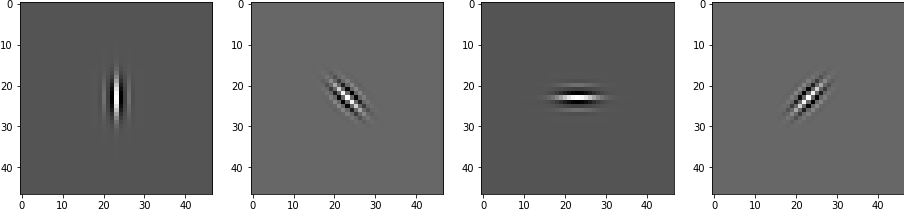
\includegraphics[width=0.5\textwidth,keepaspectratio]{images/gen/tsugf_filters/filters.png}
	\captionsetup{width=0.5\textwidth,format=plain}
	\caption{Zum texturbasierten Clustering genutze Filterbank}
	\label{fig:tsugf_filters}
\end{figure}

Diese werden anschließend über das in den Unterabschnitten~\ref{ssec:convolution} und \ref{ssec:convolutional_layer} beschriebene Konvolutionsverfahren angewandt. Dieser Vorgang resultiert in einem Datenwürfel, bei welchem die ersten beiden Dimensionen gleich der Höhe und Breite der Eingabebilddatei sind, und die dritte Dimension gleich der Anzahl der genutzten Filter ist. Somit enthält jede Schicht des Würfels Informationen darüber, wie sehr und wo im Bild das Muster der jeweiligen Filterbank \enquote{erkannt} wird. Dies ist in \figurename~\ref{fig:tsugf_101027_raw} sichtbar.

\begin{figure}[h!]
	\begin{subfigure}[t]{0.32\textwidth}
		\centering
		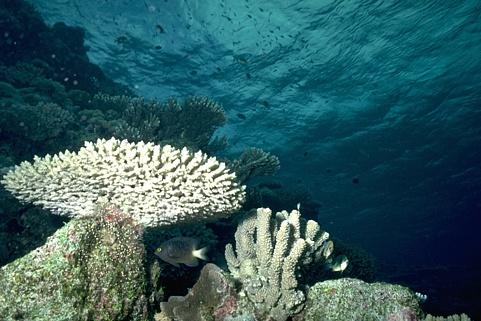
\includegraphics[width=\textwidth,keepaspectratio]{images/bsd/101027.jpg}
		\captionsetup{format=plain}
		\subcaption{}
		\label{fig:bsd_101027}
	\end{subfigure}
	\hfill
	\begin{subfigure}[t]{0.32\textwidth}
		\centering
		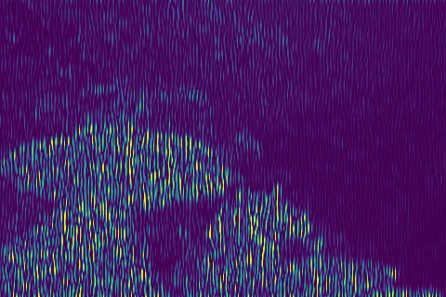
\includegraphics[width=\textwidth,keepaspectratio]{images/gen/convolution/101027.jpg_0.png}
		\subcaption{}
	\end{subfigure}
	\hfill
	\begin{subfigure}[t]{0.32\textwidth}
		\centering
		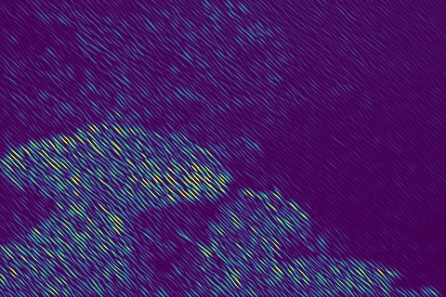
\includegraphics[width=\textwidth,keepaspectratio]{images/gen/convolution/101027.jpg_1.png}
		\subcaption{}
	\end{subfigure}
	\hfill
	\begin{subfigure}[t]{0.32\textwidth}
		\centering
		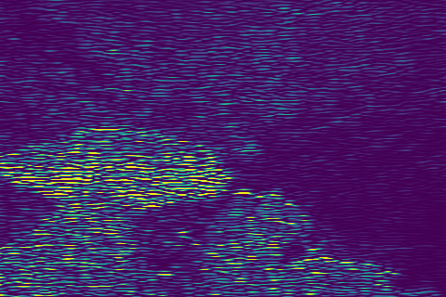
\includegraphics[width=\textwidth,keepaspectratio]{images/gen/convolution/101027.jpg_2.png}
		\subcaption{}
	\end{subfigure}
	\hfill
	\begin{subfigure}[t]{0.32\textwidth}
		\centering
		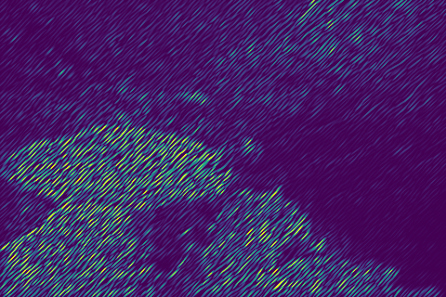
\includegraphics[width=\textwidth,keepaspectratio]{images/gen/convolution/101027.jpg_3.png}
		\subcaption{}
	\end{subfigure}
	\hfill
	\begin{subfigure}[t]{0.32\textwidth}
		\hfill
	\end{subfigure}
	\caption{Ergebnisse (b-e) der Konvolution des Beispielbildes (a, aus \cite{bsd500}) mit den jeweiligen Filtern}
	\label{fig:tsugf_101027_raw}
\end{figure}

Ähnlich zur Vorgehensweise von SLIC wird dem werden dem Datenwürfen zusätzliche Informationen über die jeweiligen X- und Y-Koordinaten hinzugefügt. Anschließend wird der k-Means-Algorithmus auf diesen Datenwürfel angewandt, es werden also Pixel mit ähnlichen Texturen und geringer Distanz zueinander in Cluster zusammengefasst.

In der Praxis sind für die erfolgreiche Anwendung dieser Methode allerdings noch einige Optimierungen notwendig: \cite{mathworks_15}

\paragraph{Weichzeichnung}
Da die Anwendung des Konvolutionsverfahrens wie in \figurename~\ref{fig:tsugf_101027_raw} sichtbar zu einer streifenartigen Merkmalsextraktion führen kann, macht es in vielen Fällen Sinn, die jeweiligen Merkmalsebenen weichzuzeichnen. Als Radius eignet sich hier ein Wert, welcher groß genug ist um die Streifen zu entfernen, aber klein genug ist, als dass die Ränder der jeweiligen erkannten Texturen nicht in benachbarte Texturen überfließen.
\paragraph{Räumlicher Bezug}
Damit diese Cluster eine (bessere) räumliche Beziehung zueinander haben, wird zu den Merkmalsdimensionen je eine Schicht hinzugefügt, welche ausschließlich mit den X-Koordinaten der jeweiligen Pixel gefüllt ist. Selbiges geschieht für die jeweiligen Y-Koordinaten. Da diese vom k-Means Algorithmus auch zusammen geclustert werden, entsteht ein örtlicher Bezug unter den Clustern. Dies wurde auch in der ursprünglichen Ausarbeitung \cite{jain_91} berücksichtigt.
\paragraph{Normalisierung}
Die jeweiligen Schichten sollten vor der Anwendung des k-Means-Algorithmus normalisiert werden um zu vermeiden, dass manche Merkmale stärer gewichtet werden als andere. Dies ist insbesondere wichtig, wenn wie oben genannt die Farb- oder Positionswerte den Merkmalsdimensionen hinzugefügt werden, da diese sich oft auf unterschiedlichen Skalen gegenüber den Konvolutionsergebnissen befinden.
\paragraph{Farbdimensionen}
Wenn die Eingabedatei eine RGB-Aufnahme ist, können diese drei Farbkanäle zur besseren Unterscheidung von unterschiedlichen Clustern mit ähnlichen Texturen genutzt werden. Dazu wird die Aufnahme in ihre drei Farbkanäle aufgeteilt und diese drei Schichten anschließend als Merkmalsdimensionen dem Datenwürfel hinzugefügt. Obwohl dies nicht in \cite{jain_91} aufgeführt wird, ist es in manchen Anwendungsbereichen zur gängigen Praxis geworden.

\paragraph{}
Das schrittweise Hinzufügen dieser Optimierungen ist in \figurename~\ref{fig:tsugf_optim} sichtbar.

\begin{figure}[h!]
	\begin{subfigure}[t]{0.32\textwidth}
		\centering
		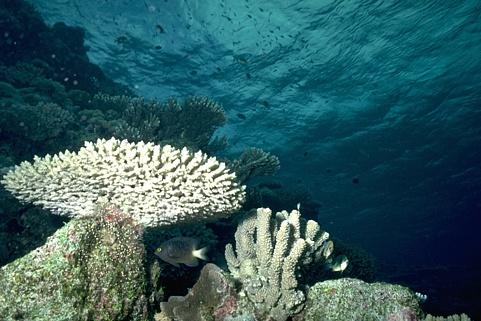
\includegraphics[width=\textwidth,keepaspectratio]{images/bsd/101027.jpg}
		\subcaption{Beispielbild (aus \cite{bsd500})\\\xspace}
	\end{subfigure}
	\hfill
	\begin{subfigure}[t]{0.32\textwidth}
		\centering
		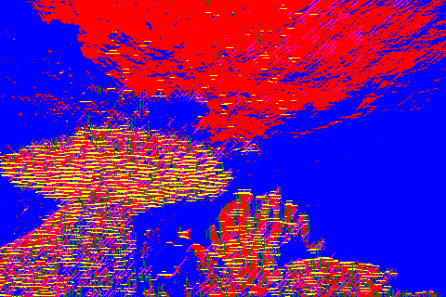
\includegraphics[width=\textwidth,keepaspectratio]{images/gen/optims/101027.jpg_raw.png}
		\captionsetup{format=plain}
		\subcaption{Originales Clusteringergebnis\\\xspace}
	\end{subfigure}
	\hfill
	\begin{subfigure}[t]{0.32\textwidth}
		\centering
		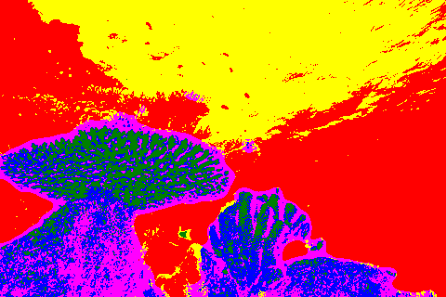
\includegraphics[width=\textwidth,keepaspectratio]{images/gen/optims/101027.jpg_blur.png}
		\subcaption{Weichzeichnen der Konvolutionsergebnisse}
	\end{subfigure}
	\hfill
	\begin{subfigure}[t]{0.32\textwidth}
		\centering
		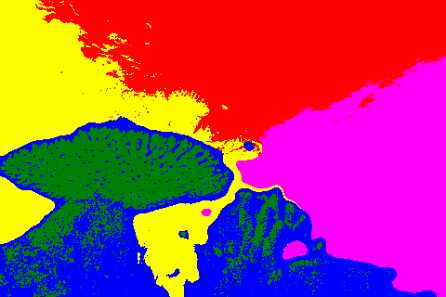
\includegraphics[width=\textwidth,keepaspectratio]{images/gen/optims/101027.jpg_blur_norm_spatial.png}
		\subcaption{Zusätzliche räumliche Informationen und Normierung}
	\end{subfigure}
	\hfill
	\begin{subfigure}[t]{0.32\textwidth}
		\centering
		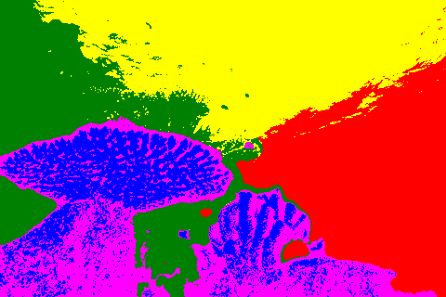
\includegraphics[width=\textwidth,keepaspectratio]{images/gen/optims/101027.jpg_blur_norm_spatial_color.png}
		\subcaption{Zusätzliche Farbinformationen}
	\end{subfigure}
	\hfill
	\begin{subfigure}[t]{0.32\textwidth}
		\hfill
	\end{subfigure}
	\caption{Optimierung des Clusteringverfahrens}
	\label{fig:tsugf_optim}
\end{figure}

Neben der in \figurename~\ref{fig:tsugf_filters} gezeigten Filterbank existieren alternative Filterbänke, \ua:
\begin{itemize}
	\item Die Leung-Malik (LM) Filterbank \cite{leung_01}
	\item Die Schmid (S) Filterbank \cite{schmid_01}
	\item Die Maximum Response (MR) Filterbank \cite{visgeo}
\end{itemize}

Diese drei Filterbänke besitzen im Gegensatz zu der in \cite{mathworks_15} vorgestellten Filterbank auch Filter in verschiedenen Größen und rotationsinvariante Filter. Sie sind in \figurename~\ref{fig:filterbank} dargestellt.

\begin{figure}[h!]
	\begin{subfigure}[t]{0.38\textwidth}
		\centering
		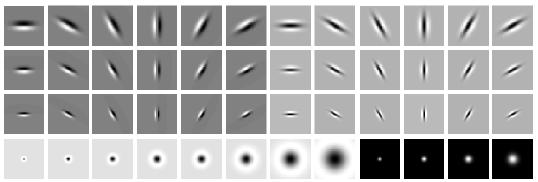
\includegraphics[width=\textwidth,keepaspectratio]{images/vis/vis_01.jpg}
		\captionsetup{format=plain}
		\subcaption{Leung-Malik-Filterbank}
	\end{subfigure}
	\hfill
	\begin{subfigure}[t]{0.38\textwidth}
		\centering
		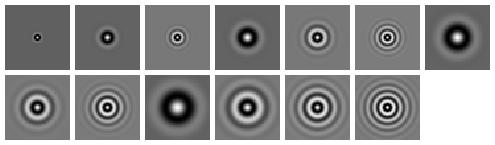
\includegraphics[width=\textwidth,keepaspectratio]{images/vis/vis_02.jpg}
		\subcaption{Schmid-Filterbank}
	\end{subfigure}
	\hfill
	\begin{subfigure}[t]{0.21\textwidth}
		\centering
		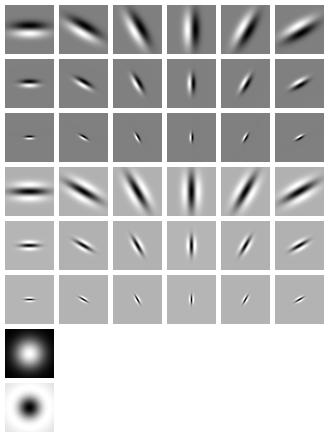
\includegraphics[width=\textwidth,keepaspectratio]{images/vis/vis_03.jpg}
		\subcaption{Maximum Response-Filterbank}
	\end{subfigure}
	\caption{Darstellung dreier Filterbänke, aus \cite{visgeo}}
	\label{fig:filterbank}
\end{figure}

Die Besonderheit der Maximum Response-Filterbank besteht daraus, dass sie zwar 38 Filtern besitzt, nach der Anwendung der Konvolution aber alle bis auf die 6 Filter mit der stärksten Reaktion auf die Eingabe an den k-Means-Algorithmus weitergegeben werden. Zusätzlich werden immer die rotationsinvarianten Filter genutzt.

% TODO Remove?
\section{Kratererkennung}
\label{sec:crater_detection}

In \cite{bandeira_10} und dessen Fortsetzung \cite{bandeira_12} wird ein neuer Ansatz zur Kratererkennung vorgestellt. Zuvor wurden diese meist manuell katalogisiert, dies resultierte darin, dass nur die größten Krater dokumentiert wurden, oder darin, dass nur vergleichsweise kleine Bereiche innerhalb eines akzeptablen Zeitraums verarbeitet werden konnten. Daher legen die Autoren insbesondere Wert auf die korrekte Erkennung von kleineren Kratern.

Die erarbeitete Vorgehensweise beginnt damit, dass über einen möglichst effizienten Algorithmus (hier der Algorithmus von Urbach \etal \cite{urbach_stepinski_2009}) eine Vorsortierung von Krater-Kandidaten berechnet wird. Als Alternative zu diesem Algorithmus werden \cite{bandeira_07} und \cite{salamuniccar_10} genannt.

Der genutzte Algorithmus ist zwar relativ effizient, da er parallel alle Merkmale eliminiert, die nicht auf Krater hindeuten. Frühere Algorithmen hingegen griffen meist auf eine Brute-Force-Methode zurück. Zur Erkennung von Krater (\bzw Krater-Kandidaten) wird hier die Tatsache genutzt, dass diese auf Abbildungen meisten aus nebeneinander liegenden, starken Schatten- und Spitzlicht-Regionen bestehen.

Nach dieser Vorsortierung und Pre-Processing Schritten (in Form von Histogramm-Optimierung) werden in \cite{bandeira_10, bandeira_12} neun Bitmasken (siehe \figurename~\ref{fig:BDS12_01}) in verschiedenen Positionen, Größen und Ausrichtungen über die Kandidaten gelegt. Die Wahrscheinlichkeit, dass der Kandidat ein Krater ist, berechnet sich aus der Übereinstimmung zwischen den Bitmasken und dem eigentlichen Kandidatenbild. Abschließend werden die Ergebnisse mithilfe eines angepassten AdaBoost Algorithmus optimiert. Das Post-Processing besteht aus der Eliminierung von ungewöhnlich geformten Kratern.

\begin{figure}[h!]
	\centering
	
\includegraphics[width=.8\textwidth,keepaspectratio]{images/BDS12/BDS12_01.png}
	\caption{Die neun, zur Merkmalsextrahierung genutzen Bitmasken, aus \cite{bandeira_12}}
	\label{fig:BDS12_01}
\end{figure}

In \figurename~\ref{fig:BDS12_02} sind die von AdaBoost ausgewählten, am stärksten gewichteten Bitmasken-Überlagerungen dargestellt. Es ist zu beachten, dass der Krater im Hintergrund nur ein Beispiel ist, und nicht alle Krater, die von den jeweiligen Bitmasken überlagert werden, darstellt.

\begin{figure}[h!]
	\centering
	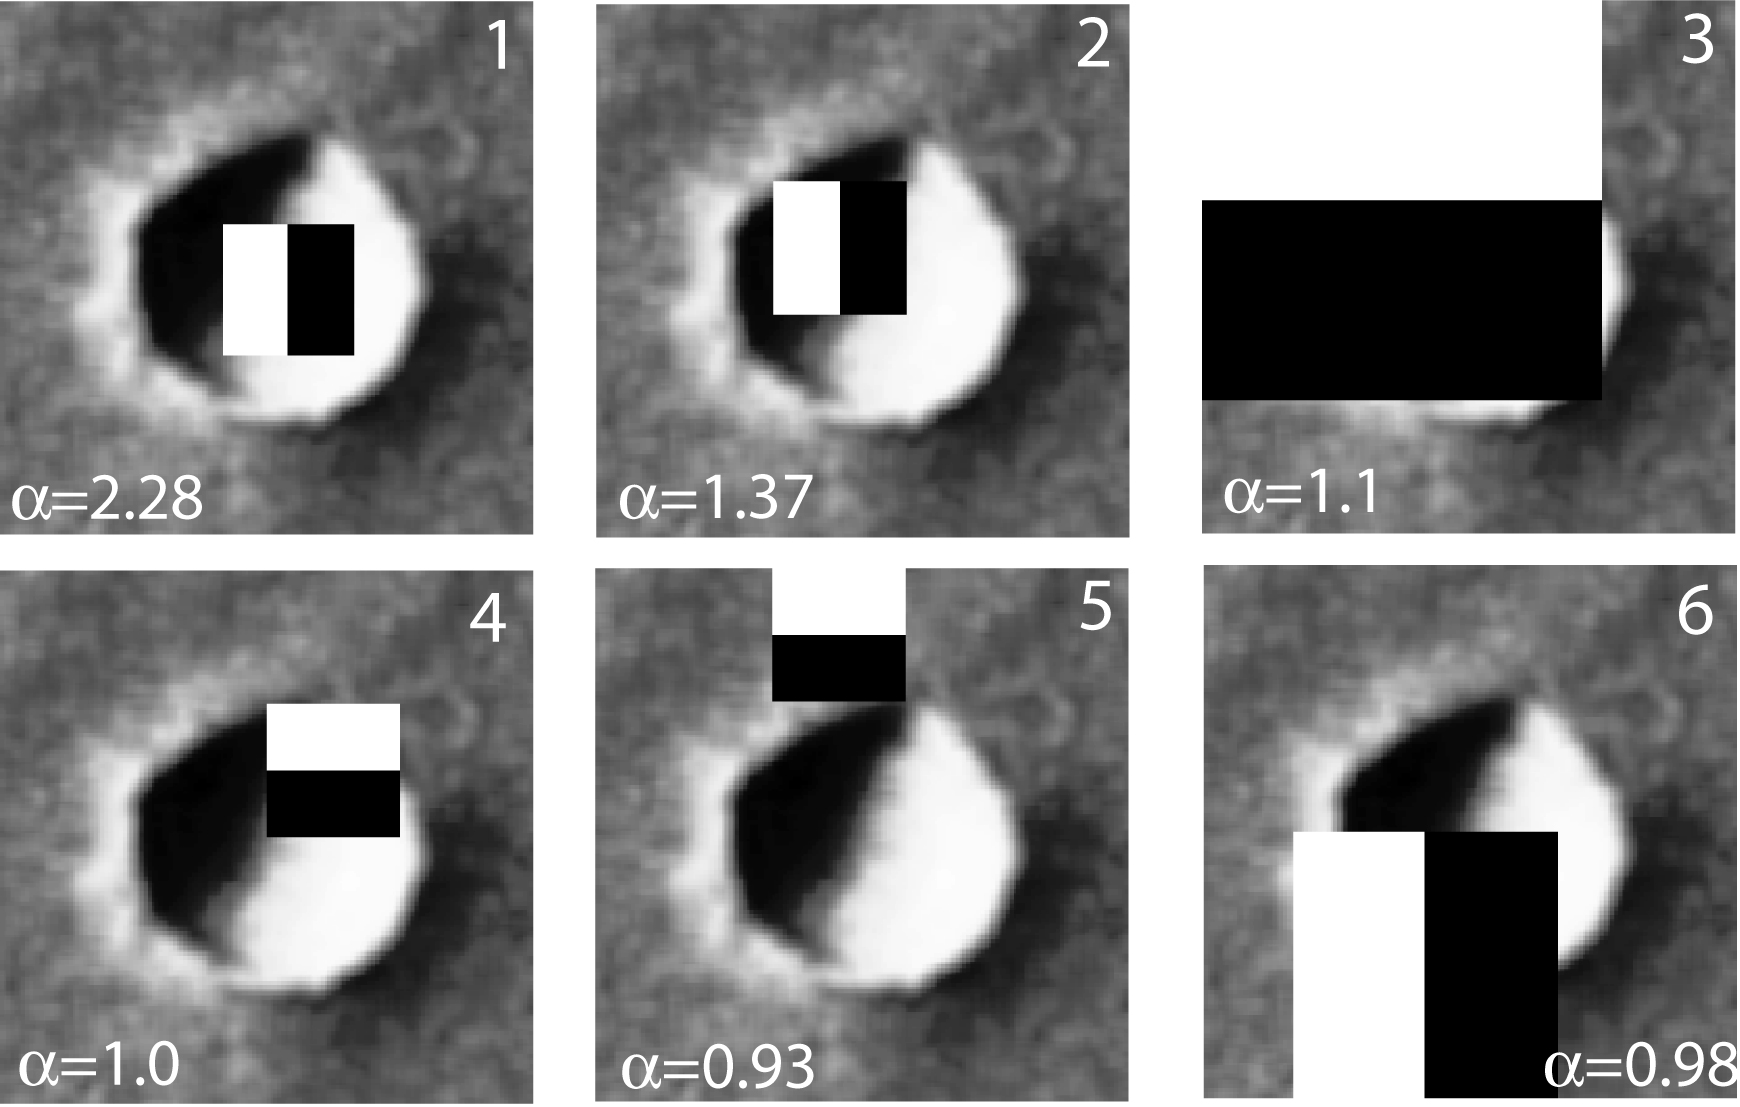
\includegraphics[width=.5\textwidth,keepaspectratio]{images/BDS12/BDS12_02.png}
	\caption{Die sechs am stärksten gewichteten Bitmasken, aus \cite{bandeira_12}}
	\label{fig:BDS12_02}
\end{figure}

\subsection{Kratererkennung über Neuronale Netze}
\label{ssec:crater_detection_nn}
Auf der Basis des erwähnten, automatisch generierten Marskrater-Datensatz, wird in \cite{cohen_16} ein neuronales Netzwerk daraufhin trainiert, selbst unterscheiden zu können, ob ein Kraterkandidat auch wirklich ein Krater ist. Die Architektur des Netzwerkes ist in \figurename~\ref{fig:CLLD16_01} zu sehen. Zur Evaluierung der Ergebnisse wird hier das 10-fache Kreuzvalidierungsverfahren genutzt. Dies bedeutet, dass der Eingabedatensatz zehn-geteilt wird, und jeweils neun Teile zum trainieren und ein Teil zum Evaluieren genutzt wird. Das Ergebnis ist der Durchschnitt der jeweiligen F1-Scores.

\begin{figure}[H]
	\centering
	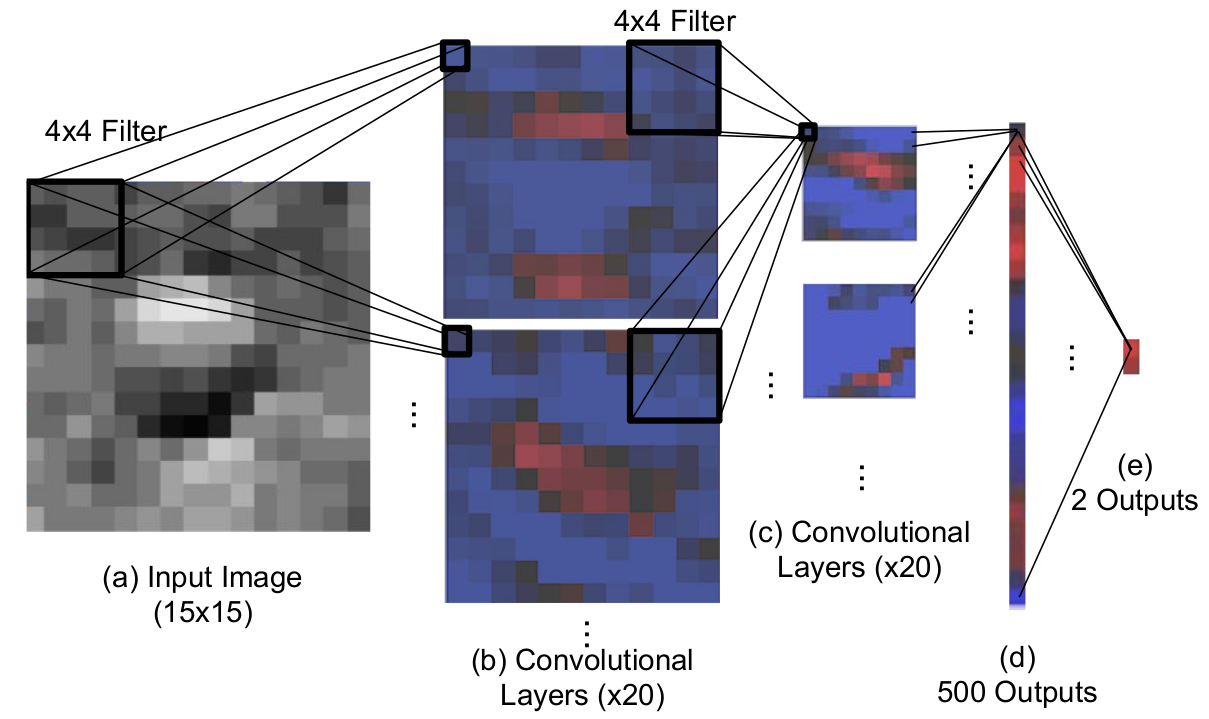
\includegraphics[width=.5\textwidth,keepaspectratio]{images/CLLD16/CLLD16_01.png}
	\caption{Die Architektur des Netzwerkes, aus \cite{cohen_16}}
	\label{fig:CLLD16_01}
\end{figure}

Der Unterschied zwischen dieser Methode und dem hier vorgestellten Ansatz besteht darin, dass in dieser Methode nur bewertet wird, ob Kraterkandidaten wirkliche Krater sind oder nicht, während hier ein Ansatz entwickelt wird, der aus einer kompletten Aufnahme der Marsoberfläche einzelne Krater(kandidaten) erkennt.

\iffalse
\subsection{Vergleich der Methoden}
\label{ssec:crater_detection_comparision}

Die drei genannten Algorithmen (Urbach '09 \cite{urbach_stepinski_2009}, Bandeira '10 \cite{bandeira_10} und Cohen '16 \cite{cohen_16}) wurden alle auf der selben Aufnahme der HRSC angewandt. Eine genauere Beschreibung und der Vergleich anhand dieser Aufnahme findet sich in Abschnitt~\ref{sec:comparision}.
\fi

\chapter{Methodik}
\label{chap:methodik}

Für die Segmentierung der Marsoberfläche wird der Ansatz von Kanezaki \etal \cite{kanezaki_18} aus Unterabschnit~\ref{ssec:kanezaki} abgewandelt. Das Ziel besteht daraus, eine Eingabebilddatei durch neuronale Netze zu segmentieren, allerdings ohne vorhandene Ground Truth.

Zur Modifikation des genannten Algorithmus existieren viele unterschiedliche Möglichkeiten, einzelne Elemente zu ersetzen, welche in den folgenden Abschnitten beschrieben werden.

\section{Funktionsweise des Algorithmus}
\label{sec:howitworks}

Die grundsätzliche Funktionsweise des Algorithmus aus \cite{kanezaki_18} findet sich in Abschnitt~\ref{ssec:kanezaki}. 

Im Folgenden gilt: $Z_F$ gibt die Menge aller durch $F$ generierten Cluster an.

Des weiteren ist $P_{F,z}$ die Menge aller Koordinaten der Pixel im Cluster $z$ der Mapping-Funktion $F$.

Der erste Schritt bei der Erstellung der Segmentierung ist die Initialisierung. Bei dieser wird ein übermäßig feines Clustering der Eingabedatei $x$ erstellt, dies geschieht über klassische Clusteringalgorithmen wie SLIC. Die Initialisierung besteht also folglich aus einer Mapping-Funktion, $I(x_{ij}), I: \mathbb{R}^p\rightarrow\mathbb{Z}$, die jedem $p$-dimensionalen Pixel $x_{ij}$ mit den Koordinaten $i$ und $j$ des Eingabebildes ein Cluster zuordnet. Der Sinn dieses initialien Clustering besteht daraus, dass das darauf folgende neuronale Netzwerk dieses nutzen kann, um zu erlernen, nach welchen Kriterien es bei der Segmentierung verfahren soll.

Dies geschieht, indem die Eingabedatei das neuronale Netzwerk durchläuft, dabei entsteht eine weitere Mapping-Funktion $F_e(x_{ij}), F: \mathbb{R}^p\rightarrow\mathbb{Z}$, wobei $e$ die Anzahl der bisherigen Epochen die das Netzwerk durchlaufen hat angibt.

Anschließend werden für jedes Cluster in $Z_{F_e}$  die Koordinaten der in ihm enthaltenen Pixel bestimmt:
\begin{equation}
P_{F_e,{z\in Z_{F_e}}} = \{\langle i, j\rangle\mid F_e(x_{ij}) = z\}
\end{equation}

Selbiges geschieht für die Initialisierung:
\begin{equation}
P_{I, z\in Z_I} = \{\langle i, j\rangle\mid I(x_{ij}) = z\}
\end{equation}

Nun wird für jedes Cluster in $Z_i$ bestimmt, welcher Wert aus $F_{e}$ am häufigsten in dem jeweiligen Cluster vorkommt, und das Cluster anschließend damit gefüllt. Das dadurch entstehende Clustering sei $F'_e$

%\begin{equation}
%\forall z\in Z_I\;\forall p\in P_{F'_e, z}\;p = %\{mod_{F_e(x_{ij})}\mid\langle i,j\rangle\in P_{I, z}\}
%\end{equation}

Anschließend wird der Loss zwischen dem ursprünglichen Ergebnis des Netzes $F_e$ und des neu generierten Ziels $F'_e$ berechnet, und eine Backpropagation über das Netzwerk ausgeführt. Dieser Prozess wird wiederholt, bis ein Abbruchkriterium (\vgl Unterabschnitt~\ref{ssec:stoppingcriteria}) erreicht wird. Er lässt sich folgendermaßen als vereinfachter Python-Code darstellen:

\begin{algorithm}
\caption{Algorithmus nach Kanezaki \etal}
\textbf{Eingabe:} Bilddatei x \\
\textbf{Ausgabe:} Clustering der Eingabebilddatei 
\begin{lstlisting}[language=Python]
def gen_cells(tags):

init_tags = slic(x)
init_coordinates = gen_clusters(init_tags)
while abbruchkriterium() is False:
	current_result = network.step(x)
	for c in init_coordinates:
		target_result[c] = mode(current_result[c])
		
	loss = CrossEntropyLoss(current_result, target_result)
	network.backpropagate()
	network.optimize()
return current_result
\end{lstlisting}
\end{algorithm}

Die insgesamt zu berechnende Mapping-Funktion ist nun das letzte erzeugte Mapping $F_e$.

Es ist zu beachten, dass für jeder Iteration die selbe Initialisierung $I$ benutzt wird.

\section{Initialisierung}
\label{sec:initialization}

Die wohl wichtigste Veränderung des ursprünglichen Algorithmus besteht aus der Modifizierung des Initialisierungsalgorithmus.

Der von Kanezaki \etal genutzte SLIC-Algorithmus eignet sich zwar gut für die meisten mehrfarbigen Fotografien, da die Aufnahmen der Marsoberfläche allerdings nur in Graustufen vorhanden sind, würden so hier keine guten Resultate produziert werden.

\begin{figure}[h!]
	\centering
	\begin{subfigure}[t]{0.32\textwidth}
		\centering
		\includegraphics[width=\textwidth,keepaspectratio]{images/Gre13/Gre13_01.jpg}
		\captionsetup{format=plain,width=0.85\textwidth}
		\caption{Eingabebild, aus \cite[Kap.~7]{greeley_13}}
		\label{fig:slic_vs_tsugf_in}
	\end{subfigure}
	\hfill
	\begin{subfigure}[t]{0.32\textwidth}
		\centering
		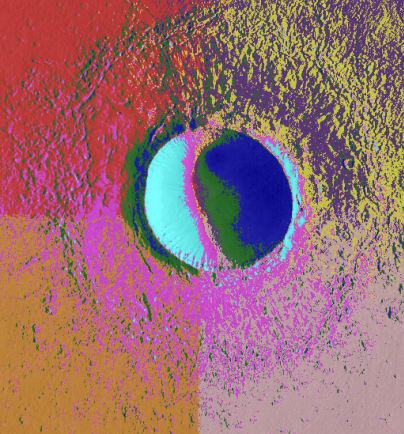
\includegraphics[width=\textwidth,keepaspectratio]{images/gen/slic_vs_tsugf/Gre13_01.jpg_slic.png}
		\captionsetup{format=plain,width=0.85\textwidth}
		\caption{Ergebnis des SLIC-Algorithmus angewandt auf die Eingabedatei}
		\label{fig:slic_vs_tsugf_slic}
	\end{subfigure}
	\hfill
	\begin{subfigure}[t]{0.32\textwidth}
		\centering
		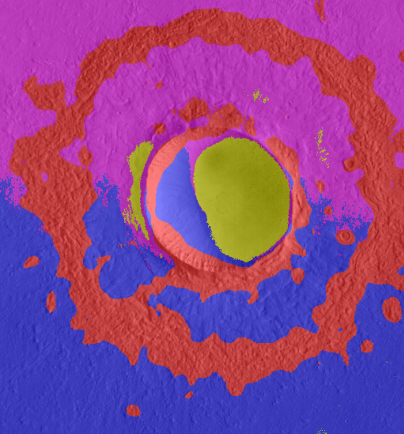
\includegraphics[width=\textwidth,keepaspectratio]{images/gen/slic_vs_tsugf/Gre13_01.jpg_tsugf.png}
		\captionsetup{format=plain,width=0.85\textwidth}
		\caption{Ergebnis des texturbasierten Clusterings der Eingabedatei}
		\label{fig:slic_vs_tsugf_tsugf}
	\end{subfigure}
	\caption{Clustering eines Graustufenbildes}
\end{figure}

So ergibt ein Clustering des Kraters aus Unterabschnitt~\ref{ssec:mars_surface_features} durch den SLIC-Algorithmus \cite{achanta_10} das in \figurename~\ref{fig:slic_vs_tsugf_slic} sichtbare Ergebnis.\footnote{SLIC-Implementierung: \texttt{scikit-image}\\Parameter: \texttt{compactness=5, n\_segments=10, enforce\_connectivity=False}} Dort ist erkennbar, dass der Krater in jeweilige Licht- und Schattenregionen (bedingt durch den Lichteinfall im flachen Winkel) unterteilt wird. Außerdem wird die raue Struktur ringförmig um den Krater herum schlecht erfasst: An dieser Stelle wird jeder Hügel separat als einerseits helle, andererseits dunkle Stelle markiert. Das Phänomen, dass ein Krater so durch eine starke Differenz an Licht- und Schattenregionen äußert wird sich im Großen und Ganzen zwar in Abschnitt~\ref{sec:craterdetection} zu nutze gemacht, ist hier allerdings ungewollt.

Wenn nun der in Unterabschnitt~\ref{ssec:kanezaki} beschriebene Ansatz verfolgt wird, wird das neuronale Netz daraufhin trainiert, eine Aufnahme anhand ihrer Helligkeitsinformationen hin zu trainieren. Da dies nicht gewollt ist, wird statt einem farb-/helligkeitsbasierten Clusteringalgorithmus wie SLIC ein texturbasiertes Clustering genutzt.

Statt des SLIC-Clusterings wird nun die in Unterabschnitt~\ref{ssec:tsugf} vorgestellte Methode des texturbasierten Clusterings genutzt. Von dieser Stelle an sind --~wenn nicht anders benannt~-- die Gewichtungen der verschiedenen Werte für die Farbwerte, X-/Y-Positionen und Reaktion auf Gaborfilter alle gleich $1$. Diese Parameter werden in Unterabschnitt~\ref{ssec:initialization_filterweight} genauer erläutert.

Das Resultat eines Clusterings durch die genutzte, texturbasierte Methode\footnote{Kombiniert mit der Filterbank aus \cite{jain_91}} ist in \figurename~\ref{fig:slic_vs_tsugf_tsugf} sichtbar: Man erkennt, dass der \enquote{Ring} um den eigentlichen Einschlagskrater eine eigenständige Textur besitzt, welche unterschiedlich zu dem Rest der Oberfläche ist. Eine ähnliche Oberflächenstruktur ist direkt um den Krater herum vorhanden. Beide Vorkommnisse dieser ähnlichen Struktur werden vom texturbasierten Clustering erfasst, in ein Segment aufgeteilt und (hier durch eine rote Färbung) markiert.

\subsection{Filterbänke}
\label{ssec:initialization_filterbanks}
Nun stellt sich die Frage, welche der vorgestellten Filterbänke sich gut eignet, die Eingabedatei zu clustern. Die größten Unterschiede zwischen den einzelnen Filterbänken besteht daraus, dass einige von ihnen rotationsinvariante Filter enthalten, und einige in mehreren Größen vorhanden sind. Die Größendifferenz lässt sich zwar in der Anwendung des Algorithmus ausgleichen, die Rotationsinvarianz allerdings nicht. In \figurename~\ref{fig:filterbank_comparision} ist die Anwendung der in Unterabschnitt~\ref{ssec:tsugf} vorgestellten Filterbänke auf vier Beispielbilder (\vgl Abschnitt~\ref{ssec:mars_surface_features}) sichtbar. Jedes Bild wurde in vier Cluster aufgeteilt und alle Optimierungen des Verfahrens (\vgl Unterabschnitt~\ref{ssec:tsugf}) wurden angewandt.

\paragraph{Krater}
Neben dem eigentlichen Krater ist auf dieser Aufnahme der Ring aus gröberem Gestein signifikant. Dieser wird von allen Filterbänken zuverlässig erkannt, wenn auch mit einer unterschiedlichen Dicke: Die LM- und S-Filterbank selektieren dieses Gestein eher großzügig, die MR-Filterbank hingegen zeigt sehr enge Markierungen dieser Region.

Alle Filterbänke formen einen Ring (oder dessen Ansatz) auf dem Kraterrand, die Maximum Response-Filterbank erzeugt zwei konzentrische Ringe

Der Krater selbst wird von den Filterkombinationen nach \cite{jain_91} und der LM-Filterbank leider nur in Hell- und Dunkel-Regionen aufgeteilt, die S-Filterbank zeigt innerhalb des Kraters kein brauchbares Ergebnis. Eine Ausnahme stellt die Maximum-Response-Filterbank dar, welche neben den zwei erwähnten konzentrischen Clustern den Bereich innerhalb des Kraters als ein einziges Cluster erkennt. Die Maximum Response-Bank erzeugt in diesem Bereich das Resultat, welches sich wohl als bestes zur Weiterverarbeitung eignet.

\paragraph{Vulkan}
Der Vulkanberg wird leider von keiner Filterbank optimal erkannt. Der äußere Rand wird nur von der S-Filterbank als ein Cluster erkannt, dies allerdings nicht sehr genau. Der rauere Bereich der Oberfläche, was kleinere Krater miteinbeschließt, wird vom MR-Filter am ehesten und genausten erkannt, auf dem zweiten Platz folgt die Filterbank nach \cite{jain_91}, welche zwar alle Krater in ein Cluster fügt (violett), allerdings eher gröber.

Die Vulkanmitte wird von keiner Filterbank erkannt, nur bei der MR-Bank lässt sich eine ringförmige, rauere Stelle um den Krater herum erahnen. Die anderen Filterbänke selektieren an dieser Stelle hauptsächlich nach den Helligkeitswerten. Außerdem ist interessant, dass der LM-Filter die Bergspitzen in vom Umfeld getrennte Cluster einteilt (blau und violett). Somit scheint es, als ließe sich diese Aufnahme über keine Filterbank gut clustern, am ehesten eignet sich allerdings erneut die MR-Bank.

\paragraph{Vulkan mit strahlenförmigen Merkmalen}

Das Ziel bei der Nutzung dieser Marsaufnahme zur Analyse besteht daraus zu analysieren, mit welcher Filterbank die konzentrischen Strahlen am genauesten erkannt werden. Des Weiteren existieren auf der Aufnahme noch Krater, welche es separat einzuordnen gilt.

Die Filterbank nach \cite{jain_91} erkennt die gröberen Strukturen (Strahlen und Krater), fügt diese allerdings in dasselbe Cluster ein (gelb und blau).

Die LM-Filterbank scheint kein brauchbares Ergebnis zu produzieren, sie erkennt im Allgemeinen nur einige der Krater (rot) separat von deren Umfeld, die Strahlen sind nicht geeignet geclustert worden.

Die Schmid-Filterbank clustert einen Großteil der Strahlen gemeinsam in ein Cluster (rot). Die Krater hingegen sind nicht fest einer Clusterart zugewiesen, ein Großteil von ihnen befindet sich jedoch auch im roten Cluster.

Wie in den vorherigen Test ist das Resultat der MR-Filterbank schon fast zu genau, die Cluster sind sehr fein gehalten. Im Gegensatz zu den Alternativen, werden hier die Krater relativ zuverlässig in gelbe Cluster eingeordnet, die Strahlen sind leider zu fein markiert, als dass man sie getrennt erkennen könnte. Dieses Phänomen könnte sich allerdings in der praktischen Anwendung zunutze gemacht werden, da dafür eine zu feine Initialisierung notwendig ist.

\paragraph{Gletscher}

Der Gletscher ist subjektiv betrachtet das schwierigste der hier vorgestellten Probleme, da er an vielen seiner Ränder keine feste Grenze zu benachbarten Regionen zeigt, nur links auf der Aufnahme ist er durch eine Hügelreihe strikt begrenzt. Diese Grenze wird von allen Filterbänken in ein getrenntes Cluster unterteilt,mit Ausnahme der Filterbank nach \cite{jain_91}: Diese produziert kein geeignetes Ergebnis, nur die stärker erkennbaren \enquote{Streifen} werden gut erkannt (violett). Die LM-Filterbank erkennt zwar die Abgrenzung auf der linken Seite, allerdings keine anderen Regionen korrekt. Sie liefert bei diesem Bild das wohl schlechteste Resultat. Die Maximum-Response Methode und die Filterbank nach \cite{schmid_01} liefern zwar etwas bessere Ergebnisse, diese sind allerdings nicht gut. Die MR-Bank erzeugt erneut sehr feine Cluster.

\paragraph{}
Zusammengefasst erzeugt aus dieser Auswahl an Filterbänden die Maximum Response-Methode von \cite{visgeo} das wohl am ehesten geeignete Resultat zur Weiterverarbeitung. Auf zweitem Platz folgt die Schmid-Filterbank.

\begin{figure}[h!]
\setlength\tabcolsep{1pt}
\def\arraystretch{0.5}
\begin{tabular}{p{0.2\textwidth}p{0.2\textwidth}p{0.2\textwidth}p{0.2\textwidth}p{0.2\textwidth}}
	\includegraphics[width=0.2\textwidth]{images/Gre13/Gre13_01.jpg} &
	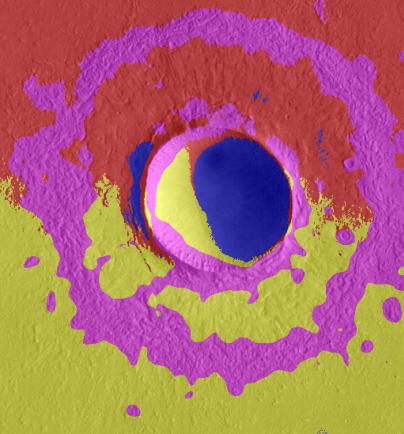
\includegraphics[width=0.2\textwidth]{images/gen/filterbanks/Gre13_01.jpg_TSUGF.png} &
	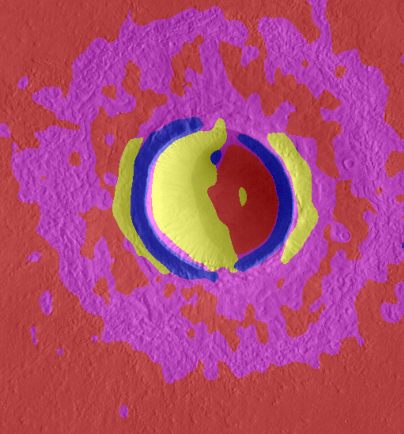
\includegraphics[width=0.2\textwidth]{images/gen/filterbanks/Gre13_01.jpg_LM.png} &
	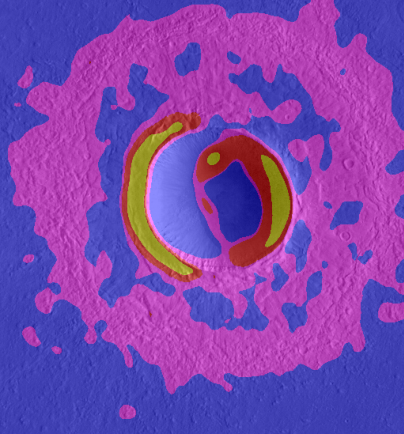
\includegraphics[width=0.2\textwidth]{images/gen/filterbanks/Gre13_01.jpg_S.png} &
	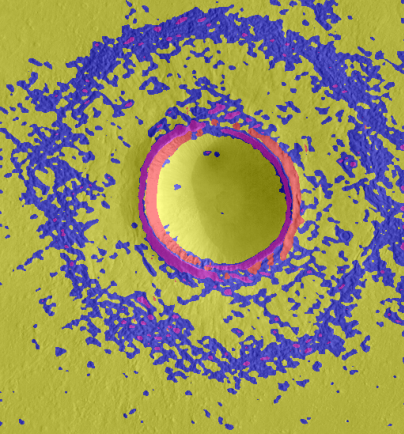
\includegraphics[width=0.2\textwidth]{images/gen/filterbanks/Gre13_01.jpg_MR.png} \\
	
	\includegraphics[width=0.2\textwidth]{images/Gre13/Gre13_02.jpg} &
	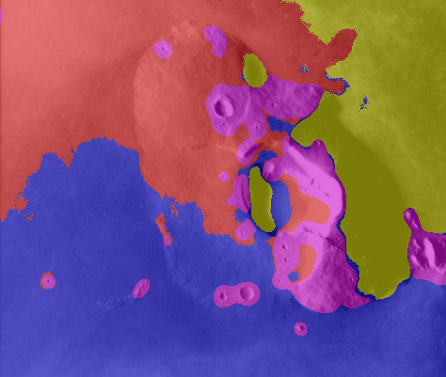
\includegraphics[width=0.2\textwidth]{images/gen/filterbanks/Gre13_02.jpg_TSUGF.png} &
	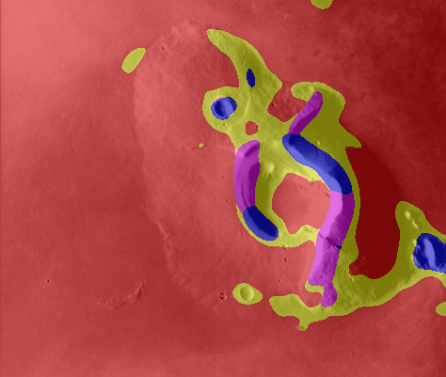
\includegraphics[width=0.2\textwidth]{images/gen/filterbanks/Gre13_02.jpg_LM.png} &
	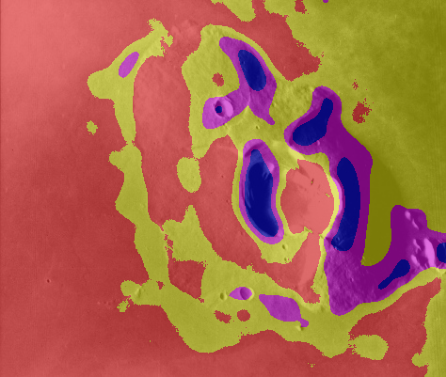
\includegraphics[width=0.2\textwidth]{images/gen/filterbanks/Gre13_02.jpg_S.png} &
	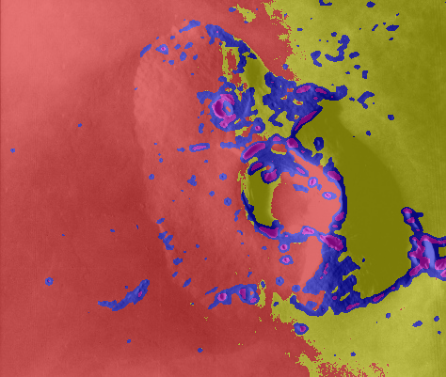
\includegraphics[width=0.2\textwidth]{images/gen/filterbanks/Gre13_02.jpg_MR.png} \\
	
	\includegraphics[width=0.2\textwidth]{images/Gre13/Gre13_03.jpg} &
	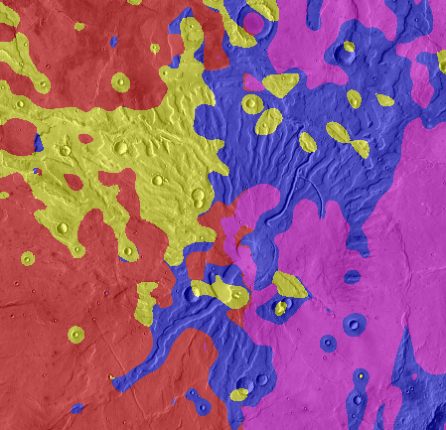
\includegraphics[width=0.2\textwidth]{images/gen/filterbanks/Gre13_03.jpg_TSUGF.png} &
	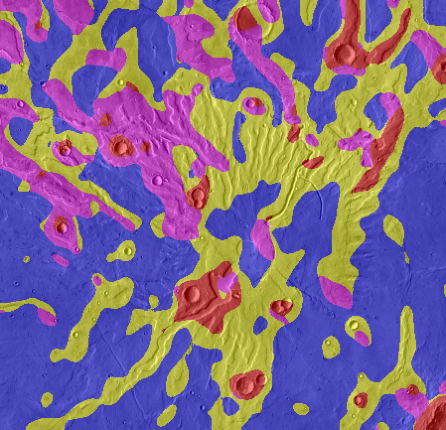
\includegraphics[width=0.2\textwidth]{images/gen/filterbanks/Gre13_03.jpg_LM.png} &
	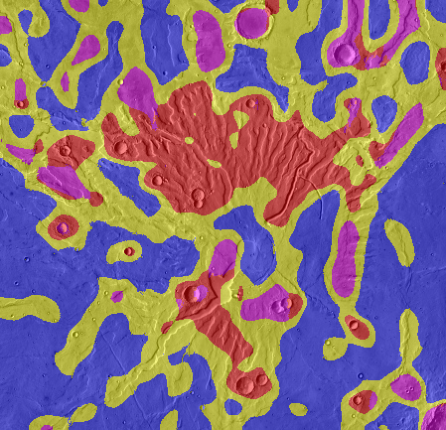
\includegraphics[width=0.2\textwidth]{images/gen/filterbanks/Gre13_03.jpg_S.png} &
	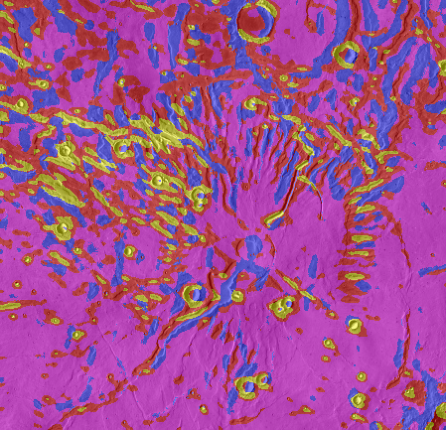
\includegraphics[width=0.2\textwidth]{images/gen/filterbanks/Gre13_03.jpg_MR.png} \\
	
	\includegraphics[width=0.2\textwidth]{images/Gre13/Gre13_05.jpg} &
	\includegraphics[width=0.2\textwidth]{images/gen/filterbanks/Gre13_05.jpg_TSUGF.png} &
	\includegraphics[width=0.2\textwidth]{images/gen/filterbanks/Gre13_05.jpg_LM.png} &
	\includegraphics[width=0.2\textwidth]{images/gen/filterbanks/Gre13_05.jpg_S.png} &
	\includegraphics[width=0.2\textwidth]{images/gen/filterbanks/Gre13_05.jpg_MR.png} \\
	
	\hspace{1pt}\newline\centering Eingabe, aus \cite{greeley_13} &
	\hspace{1pt}\newline\centering Filterbank nach \cite{jain_91} &
	\hspace{1pt}\newline\centering LM-Filterbank \cite{leung_01} &
	\hspace{1pt}\newline\centering S-Filterbank \cite{schmid_01} &
	\hspace{1pt}\newline\centering MR-Filterbank \cite{visgeo} \\
\end{tabular}
\caption{Vergleich verschiedener Filterbänke auf Bildern der Marsoberfläche (Krater, Vulkan, Vulkan mit strahlenförmigen Merkmalen, Gletscher). Die Farben der jeweiligen Cluster wurden zufällig gewählt und sagen nichts über deren Inhalt aus. Alle Bilder wurden in vier Cluster eingeteilt.}
\label{fig:filterbank_comparision}
\end{figure}

\subsection{Größe der Filter}
\label{ssec:initialization_filtersize}

Neben der Auswahl einer geeigneten Filterbank lassen sich in dieser noch die einzelnen Gewichtungen anpassen: So könnten \zB die Gewichtung der Koordinaten der Pixel zueinander oder die Relevanz von ähnlichen Farbwerten modifiziert werden. Außerdem ist die Größe der einzelnen Filter in den jeweiligen Filterbänken auch Variabel und muss dementsprechend an die Dimensionen des jeweiligen Eingabebildes angepasst werden. Da alle Filterbänke (bis auf die nach \cite{jain_91}) jeweils gleiche Filter in unterschiedlichen Größen enthalten, muss nur ein Gesamtwert angepasst werden, statt der Größe jeder einzelnen Skalierung. Es wird nun versucht, die Ergebnisse der Maximum Response-Filterbank zu verbessern, da diese in vorherigen Versuchen die besten Ergebnisse erzielt hat.

Von dieser Stelle an müssen Marsaufnahmen genutzt werden, bei denen die Auflösung bekannt ist, somit scheiden die bis hierhin genutzten Aufnahmen aus \cite{greeley_13} leider aus. Stattdessen werden Ausschnitte aus der Aufnahme \texttt{P03\_002147\_1865\_XI\_06N208W} der Context Camera des Mars Reconnaissance Orbiters genutzt. Ein weiterer Vorteil der Nutzung dieser Bilder besteht daraus, dass die Clusteringalgorithmen nun an realitätsnähreren Daten getestet werden können, statt an isolierten Aufnahmen einzelner Besonderheiten der Oberfläche. Die Ergebnisse sind in \figurename~\ref{fig:filterbank_sizes} zu sehen. Als Startwert wurde ein Skalierungsfaktor $s=1$ betrachtet, angewandt auf die vorgestellten, quadratischen Filter mit einer originalen Kantenlänge von \SI{49}{\pixel}. Dieser wurde nach oben und unten hin in Schritten von $\Delta s=0.25$ verändert, und mit der skalierten MR-Filterbank ein neues Clustering der vier Ausschnitte erstellt. Die Eingabebilder sind quadratisch und besitzen eine Seitenlänge von \SI{650}{\pixel} bei einer Auflösung von \SI{6,17}{\meter\per\pixel}. Jedes der Eingabebilder wurde erneut in vier Bereiche eingeteilt, die Farben sind zur Veranschaulichung zufällig gewählt.

\paragraph{Skalierungsfaktor $s=0,25$}

Auf der ersten Aufnahme ist, vergleichbar mit den Beispielaufnahmen aus dem letzten Abschnitt, ein runder Krater zentriert zu sehen. Die geringe Skalierung mit dem Faktor $s=0.25$ führt dazu, dass die jeweiligen Filter zu klein sind, um die Strukturen der Oberfläche zu erkennen, somit sieht diese Aufnahme aus, als wäre nur anhand ihrer Helligkeitswerten geclustert worden. Das gleiche gilt auch für die zweite und vierte Aufnahme.

Die dritte Aufnahme stellt eine relativ ebenmäßige Fläche in einem Umfeld von gröberer Oberfläche dar. Dort scheint es, als gäbe es nicht genug Kontrast um nach den Helligkeitswerten zu clustern, der Algorithmus erstellt eine Filterung anhand der X- und Y-Koordinaten. Bei allen Aufnahmen werden nur zwei wirkliche Cluster erstellt, die letzten zwei Cluster die erstellt werden sollten bestehen nur aus jeweils wenigen Pixeln.

Dieser Skalierungsfaktor produziert keine brauchbaren Ergebnisse.

\paragraph{Skalierungsfaktor $s=0,50$}

Wie zu erwarten führt die genutzte, noch relativ geringe Skalierung der Filterbank mit $s=0,50$ zu vielen kleineren Clustern, in diesem Fall auf der ersten Aufnahme deutlich erkennbar anhand der gelb markierten Flächen. Obwohl es auf den ersten Blick scheint, als würden die Kraterränder erkannt werden, werden durch die Filterbank bei dieser Skalierung nur die dunkleren Bereiche, in diesem Fall die Schatten, die die erhöhten Kraterränder werfen, erkannt. Auf dieser Aufnahme führt dies zwar zu einer vergleichsweise guten Approxmimation der Krater, sobald anderweitige Schatten hinzukommen, wird diese Skalierung allerdings keine geeigneten Resultate produzieren.

Das selbe Phänomen tritt bei der zweiten Aufnahme auf, auch dort wird stark anhand der Helligkeitswerte geclustert, erkennbar insbesondere an den violetten Bereichen an den Kraterrändern. Bei diesem Bild wird allerdings auch trotz der kleineren Skalierung das raue Gebiet, welches sich horizontal durch das Bild erstreckt, in ein (rot gefärbtes) Cluster eingeteilt. Auch hier werden allerdings dunklerere Bereiche (wie die Kraterränder) in separate (violett gefärbte) Cluster eingeteilt.

Auf der dritten Aufnahme wird bei der genutzten Skalierung die feinere Fläche größtenteils als ein (gelb gefärbtes) Cluster dargestellt, separat dazu sind in rot die Übergänge zwischen den Regionen gekennzeichnet. Die gröberen Flächen in den äußeren Bereichen werden nicht zuverlässig in das selbe Cluster eingeordnet.

Die letzte Testaufnahme, bestehend aus zwei Hügeln \bzw Bergen, stellt durch die über- und unterbelichteten Flächen an den Hängen eine der größten Herausforderungen für den Clusteringalgorithmus dar. An diesen Stellen ist der Kontrast des Bildes sehr gering, sodass kaum noch Texturen erkannt werden, anhand derer geclustert werden könnte. Wie zu erwarten werden die dunklen Flächen in ein einzelnes (rotes) Cluster kombiniert. Kleine Hügelketten hingegen werden zuverlässig in zusammengehörige Cluster eingeteilt, welches auf diesen Aufnahmen blau markiert ist. Die beleuchteten Seiten der Hügel werden bei dieser Skalierung leider nicht von der allgemeinen Marsoberfläche unterschieden, höchstens der Fuß des Berges kann durch die violette Färbung erahnt werden.

Dieser Skalierungsfaktor führt zu vergleichsweise guten Clusteringergebnissen.

\paragraph{Skalierungsfaktor $s=0,75$}

Dieser Skalierungsfaktor führt beim Clustering des ersten Bildes zu Resultat, welche vergleichbar mit denen des Faktors $s=0,5$ sind. Die Ränder der Krater werden allerdings getrennt in helle und dunkle Regionen eingeteilt, die Cluster im äußeren Bereich sind größer und gröber.

Auf der zweiten Aufnahme wird die horizontale rauere Region sehr gut in ein eigenes Cluster eingeteilt, selbiges gilt für die Kraterränder. Auf dieser Aufnahme erscheint der Skalierungsfaktor $s=0,75$ für diese Filterbank optimal.

Die dritte Aufnahme unterscheidet sich bis auf die gröberen, größeren Cluster in den äußeren Bereichen nicht wesentlich von der vorherigen Skalierung.

Bei der letzten Aufnahme führt die größere Skalierung zu einem uniformen Clusterings des beleuchteten Berghangs, er wird als eine große Fläche erkannt. Die dunkle Seite hingegen wird in zwei Cluster unterteilt: Die eigentliche dunkle Seite des Berges, und die Stellen, welche zu unterbelichtet sind, um aus ihnen eine Textur zu erkennen.

Insgesamt scheint sich dieser Skalierungsfaktor auch zum textutbasierten Clustering zu eignen.

\paragraph{Skalierungsfaktor $s=1.00$}

Während bei diesem Skalierungsfaktor auf der ersten Aufnahme der größere, mittige Krater relativ gut durch ein gelbes kreisförmiges Cluster gekennzeichnet wird, wird der kleinere Krater nicht zuverlässig erkannt. Bei diesem gehen die Cluster in umlegende Gebiete über, als wäre dieser Krater nur eine etwas rauere Oberflächenstruktur.

Bei der zweiten Aufnahme wird wie zuvor der Krater erfolgreich separat in ein Cluster eingeteilt, die Begrenzungen der gröberen Struktur, welche sich durch das Bild zieht, geht allerdings verloren. Diese Region wird leider im rechten Teil des Bildes sehr weitläufig erkannt.

In dem dritten Testbild werden die gröberen Hügelketten am Rand des helleren Bereiches zwar erkannt (gelb markiert), und die Übergangsstellen zwischen zwei Regionen werden in ein blaues Cluster zusammengefügt, alle anderen Regionen sind allerdings nicht voneinander getrennt worden.

Das letzte Bild wird bei dieser Skalierung fast identisch zu der Skalierung mit $s=0,75$ geclustert.

Zusammengefasst ist diese Skalierung schon zu grob um so gute Ergebnisse wie die vorherigen zu erreichen.

\paragraph{Skalierungsfaktor $s=1.25$ und $s=1.50$}

Da diese beiden Skalierungsfaktoren zu fast identischen Clusterverteilungen führen, werden sie in einen Abschnitt zusammengefasst.

Bei diesen Skalierungen werden im oberen, glätteren Bereich der ersten Aufnahme die vereinzelten Krater wie gewollt erkannt, sie versagt allerdings im unteren, gröberen Bereich, wo sie nur ein großes Cluster erstellen. Der Krater wird nur anhand von starken Helligkeitsdifferenzen erkannt, welche in der gesamten Ausgabe gelb bei $s=1,25$, \bzw violett bei $s=1,5$ markiert wurden. 

Selbiges gilt im Bezug auf die starken Helligkeitsdifferenzen bei der zweiten Aufnahme.

Bei der dritten Aufnahme wird von beiden Skalierungsfaktoren kein brauchbares Resultat produziert, man kann höchstens erahnen, dass die gelb \bzw violett gefärbten Regionen besonders kontrastarme, also glatte Flächen darstellen sollen.

Beim Clusteringergebnis der letzten Aufnahme unterschieden sich die beiden Skalierungsfaktoren erstmals stärker: Bei $s=1,25$ gleicht das Ergebnis dem des vorherigen Clusterings: Kleinere Bergregionen und rauere Oberflächenstrukturen werden getrennt voneinander erkannt, Flächen mit weniger oder (aufgrund von Unterbelichtung) keiner werden auch in ein großes Cluster hinzugefügt. Der Faktor $s=1,5$ scheint selbst bei diesem Bild zu groß zu sein, bis auf die Hügelketten mit starker Helligkeitsdifferenz wird die Aufnahme nur anhand ihrer Helligkeitswerte geclustert.

Diese Faktoren sind also zu groß um brauchbare Resultate zu produzieren.

\begin{figure}[h!]
	\setlength\tabcolsep{1pt}
	\def\arraystretch{0.5}
	\begin{tabular}{C{0.14\textwidth}C{0.14\textwidth}C{0.14\textwidth}C{0.14\textwidth}C{0.14\textwidth}C{0.14\textwidth}C{0.14\textwidth}}
		\includegraphics[width=0.14\textwidth]{images/p03/p03_01.png} &
		\includegraphics[width=0.14\textwidth]{images/gen/filter_size/p03_01.png_0.25.png} &
		\includegraphics[width=0.14\textwidth]{images/gen/filter_size/p03_01.png_0.50.png} &
		\includegraphics[width=0.14\textwidth]{images/gen/filter_size/p03_01.png_0.75.png} &
		\includegraphics[width=0.14\textwidth]{images/gen/filter_size/p03_01.png_1.00.png} &
		\includegraphics[width=0.14\textwidth]{images/gen/filter_size/p03_01.png_1.25.png} &
		\includegraphics[width=0.14\textwidth]{images/gen/filter_size/p03_01.png_1.50.png} \\
		\includegraphics[width=0.14\textwidth]{images/p03/p03_02.png} &
		\includegraphics[width=0.14\textwidth]{images/gen/filter_size/p03_02.png_0.25.png} &
		\includegraphics[width=0.14\textwidth]{images/gen/filter_size/p03_02.png_0.50.png} &
		\includegraphics[width=0.14\textwidth]{images/gen/filter_size/p03_02.png_0.75.png} &
		\includegraphics[width=0.14\textwidth]{images/gen/filter_size/p03_02.png_1.00.png} &
		\includegraphics[width=0.14\textwidth]{images/gen/filter_size/p03_02.png_1.25.png} &
		\includegraphics[width=0.14\textwidth]{images/gen/filter_size/p03_02.png_1.50.png} \\
		\includegraphics[width=0.14\textwidth]{images/p03/p03_03.png} &
		\includegraphics[width=0.14\textwidth]{images/gen/filter_size/p03_03.png_0.25.png} &
		\includegraphics[width=0.14\textwidth]{images/gen/filter_size/p03_03.png_0.50.png} &
		\includegraphics[width=0.14\textwidth]{images/gen/filter_size/p03_03.png_0.75.png} &
		\includegraphics[width=0.14\textwidth]{images/gen/filter_size/p03_03.png_1.00.png} &
		\includegraphics[width=0.14\textwidth]{images/gen/filter_size/p03_03.png_1.25.png} &
		\includegraphics[width=0.14\textwidth]{images/gen/filter_size/p03_03.png_1.50.png} \\
		\includegraphics[width=0.14\textwidth]{images/p03/p03_04.png} &
		\includegraphics[width=0.14\textwidth]{images/gen/filter_size/p03_04.png_0.25.png} &
		\includegraphics[width=0.14\textwidth]{images/gen/filter_size/p03_04.png_0.50.png} &
		\includegraphics[width=0.14\textwidth]{images/gen/filter_size/p03_04.png_0.75.png} &
		\includegraphics[width=0.14\textwidth]{images/gen/filter_size/p03_04.png_1.00.png} &
		\includegraphics[width=0.14\textwidth]{images/gen/filter_size/p03_04.png_1.25.png} &
		\includegraphics[width=0.14\textwidth]{images/gen/filter_size/p03_04.png_1.50.png} \\
		
		\hspace{2pt}\newline\centering Eingabe & 
		\hspace{2pt}\newline\centering $s=0,25$ &
		\hspace{2pt}\newline\centering $s=0,50$ &
		\hspace{2pt}\newline\centering $s=0,75$ &
		\hspace{2pt}\newline\centering $s=1,00$ &
		\hspace{2pt}\newline\centering $s=1,25$ &
		\hspace{2pt}\newline\centering $s=1,50$
	\end{tabular}
	\caption{Vergleich verschiedener Skalierungen der MR-Filterbank auf Bildern der Marsoberfläche. Die Farben der jeweiligen Cluster wurden zufällig gewählt und sagen nichts über deren Inhalt aus. Alle Bilder wurden in vier Cluster eingeteilt.}
	\label{fig:filterbank_sizes}
\end{figure}

\paragraph{}
Aus diesen Ergebnissen lässt sich schlussfolgern, dass sich die Skalierungsfaktoren $s=0,5$ und $s=0,75$ bei diesen Eingabedaten die besten Resultate liefert. Da durch die nachfolgende Weiterverarbeitung durch den Algorithmus nach Kanezaki eine hohe Anzahl an Clustern benötigt wird, diese aber nicht zu klein und Verstreut ausfallen sollten, wird von nun an ein Skalierungsfaktor von $s=0,75$ genutzt.

\subsection{Gewichtungen der Parameter}
\label{ssec:initialization_filterweight}

Da in dem Prozess des Clusterings alle Optimierungen aus Unterabschnitt~\ref{ssec:tsugf} miteingeschlossen sind, beinhaltet dies, dass der Datenwürfel, den k-Means verarbeitet, sowohl die Koordinaten, als auch die Farbwerte der Eingabedatei beinhaltet. Nun stellt sich die Frage, wie stark diese jeweils gewichtet werden sollten, um ein akzeptables Ergebnis zu erhalten. Aus diesem Grund sind in den Abbildungen~\ref{fig:filterbank_weights_pos} und \ref{fig:filterbank_weights_col} die Resultate des Clusterings mit unterschiedlichen Werten für die jeweiligen Gewichtungen zu sehen. Die Skalierung der Filter beträgt $s=0,5$, da im vorherigen Unterabschnitt festgestellt wurde, dass dieser Wert relativ gute Ergebnisse liefert.

\paragraph{Gewichtung der Koordinaten}
Das Hinzufügen der X- und Y-Koordinaten zu dem Datenwürfel ist ursprünglich aus dem Grund geschehen, dass ein gegebener räumlicher Bezug zwischen unterschiedlichen Pixeln beim Clustering berücksichtigt werden kann (\vgl Unterabschnitt~\ref{ssec:tsugf}; \cite{jain_91}). Aus den Clusteringergebnissen in \figurename~\ref{fig:filterbank_weights_pos} allerdings lässt sich erkennen, dass dieser räumliche Bezug in diesem Anwendungsfall nicht außerordentlich hilfreich ist: Bei einer Gewichtung von $w_p\geq1,33$ lässt sich eindeutig erkennen, dass der allgemeine Bodenbereich auf allen Aufnahmen zu stark Anhand seiner Positionen eingeteilt wird, es entstehen Cluster in den Ecken der Aufnahmen, welche sich ins Zentrum erstrecken. Unter diesem starken Einfluss nimmt zusätzlich die relative Wichtigkeit der ähnlichen Textur ab.

Wird nun ein geringerer Wert für $w_p$ betrachtet, so erkennt man für Werte mit $w_p\leq0.66$ keinen Starken Unterschied bei wechselnden Gewichtungen. Dies ist insbesondere bei $w_p=0$ signifikant, da dort der räumliche Bezug der einzelnen Pixel zueinander bei der Berechnung des Clusterings zwar komplett ignoriert wird, das eigentliche Ergebnis sich --~bis auf etwas kleinere Cluster in den merkmalsarmen Bereichen~-- aber kaum verändert. Dies lässt sich darauf zurückführen, dass das Hinzufügen des räumlichen Bezuges ursprünglich den Grund hatte, dass auf \enquote{normalen} Fotografien die vorkommenden Cluster meistens nur ein einziges mal an einem räumlich begrenzten Ort vorhanden sind, so sind \zB bei der Aufnahme aus \figurename~\ref{fig:tsugf_optim} aus Unterabschnitt~\ref{ssec:tsugf} die kleineren Korallen im linken Hintergrund nur an dieser Stelle vorhanden und ließen sich durch ein weit ausgedehntes Cluster zusammenfassen. Bei den aktuell genutzten Aufnahmen hingegen ist dies nicht der Fall, eine auftretende Oberflächenstruktur, wie \zB ein Krater kann an verschieden Stellen ohne räumlichen Bezug zueinander auftreten.
Die Nutzung der Positionwerte hat allerdings einen Vorteil: Sie sorgt dafür die Clustergrößen nicht zu klein und fragmentiert werden zu lassen, indem sie eine Relation mit benachbarten Pixeln erzeugt, welche der k-Means Algorithmus berücksichtigt.

Aus diesem Grund macht es Sinn, die Koordinatenbeträge der Pixel relativ gering zu gewichten, um dafür zu sorgen, dass das texturbasierte Clustering möglicht positionsinvariant operiert, aber auch nicht so gering, dass viele fragmentierte Cluster entstehen. Anhand von \figurename~\ref{fig:filterbank_weights_pos} ist erkennbar, dass ein Wert von  $w_p=0,66$ sich in diesem Fall sehr gut eignet, ein brauchbares Clusterergebnis zu erstellen.

\begin{figure}[h!]
	\setlength\tabcolsep{1pt}
	\def\arraystretch{0.5}
	\begin{tabular}{C{0.14\textwidth}C{0.14\textwidth}C{0.14\textwidth}C{0.14\textwidth}C{0.14\textwidth}C{0.14\textwidth}C{0.14\textwidth}}
		\includegraphics[width=0.14\textwidth]{images/p03/p03_01.png} &
		\includegraphics[width=0.14\textwidth]{images/gen/spatial_weight/p03_01.png_0.00.png} &
		\includegraphics[width=0.14\textwidth]{images/gen/spatial_weight/p03_01.png_0.33.png} &
		\includegraphics[width=0.14\textwidth]{images/gen/spatial_weight/p03_01.png_0.66.png} &
		\includegraphics[width=0.14\textwidth]{images/gen/spatial_weight/p03_01.png_1.00.png} &
		\includegraphics[width=0.14\textwidth]{images/gen/spatial_weight/p03_01.png_1.33.png} &
		\includegraphics[width=0.14\textwidth]{images/gen/spatial_weight/p03_01.png_1.66.png} \\
		\includegraphics[width=0.14\textwidth]{images/p03/p03_02.png} &
		\includegraphics[width=0.14\textwidth]{images/gen/spatial_weight/p03_02.png_0.00.png} &
		\includegraphics[width=0.14\textwidth]{images/gen/spatial_weight/p03_02.png_0.33.png} &
		\includegraphics[width=0.14\textwidth]{images/gen/spatial_weight/p03_02.png_0.66.png} &
		\includegraphics[width=0.14\textwidth]{images/gen/spatial_weight/p03_02.png_1.00.png} &
		\includegraphics[width=0.14\textwidth]{images/gen/spatial_weight/p03_02.png_1.33.png} &
		\includegraphics[width=0.14\textwidth]{images/gen/spatial_weight/p03_02.png_1.66.png} \\
		\includegraphics[width=0.14\textwidth]{images/p03/p03_03.png} &
		\includegraphics[width=0.14\textwidth]{images/gen/spatial_weight/p03_03.png_0.00.png} &
		\includegraphics[width=0.14\textwidth]{images/gen/spatial_weight/p03_03.png_0.33.png} &
		\includegraphics[width=0.14\textwidth]{images/gen/spatial_weight/p03_03.png_0.66.png} &
		\includegraphics[width=0.14\textwidth]{images/gen/spatial_weight/p03_03.png_1.00.png} &
		\includegraphics[width=0.14\textwidth]{images/gen/spatial_weight/p03_03.png_1.33.png} &
		\includegraphics[width=0.14\textwidth]{images/gen/spatial_weight/p03_03.png_1.66.png} \\
		\includegraphics[width=0.14\textwidth]{images/p03/p03_04.png} &
		\includegraphics[width=0.14\textwidth]{images/gen/spatial_weight/p03_04.png_0.00.png} &
		\includegraphics[width=0.14\textwidth]{images/gen/spatial_weight/p03_04.png_0.33.png} &
		\includegraphics[width=0.14\textwidth]{images/gen/spatial_weight/p03_04.png_0.66.png} &
		\includegraphics[width=0.14\textwidth]{images/gen/spatial_weight/p03_04.png_1.00.png} &
		\includegraphics[width=0.14\textwidth]{images/gen/spatial_weight/p03_04.png_1.33.png} &
		\includegraphics[width=0.14\textwidth]{images/gen/spatial_weight/p03_04.png_1.66.png} \\
		
		\hspace{2pt}\newline\centering Eingabe & 
		\hspace{2pt}\newline\centering $w_p=0,00$ &
		\hspace{2pt}\newline\centering $w_p=0,33$ &
		\hspace{2pt}\newline\centering $w_p=0,66$ &
		\hspace{2pt}\newline\centering $w_p=1,00$ &
		\hspace{2pt}\newline\centering $w_p=1,33$ &
		\hspace{2pt}\newline\centering $w_p=1,66$
	\end{tabular}
	\caption{Vergleich verschiedener Gewichtungen der Koordinaten beim Clustering der jeweiligen Eingabedateien. Die Farben der jeweilgen Cluster wurden zufällig gewählt und sagen nichts über deren Inhalt aus. Alle Bilder wurden in vier Cluster eingeteilt.}
	\label{fig:filterbank_weights_pos}
\end{figure}

\paragraph{Gewichtungen der Farb-/Helligkeitswerte}
Die hier folgenden Clusteringergebnisse wurden mit einem Skalierungsfaktor von $s=0,5$ und einer Gewichtung von $w_p=0,66$ für die Positionswerte erstellt.

In der originalen Ausarbeitung des texturbasierten Clusterings \cite{jain_91} werden nur zwei Ebenen für die jeweiligen X- und Y-Koordinaten hinzugefügt. Es steht also an dieser Stelle offen, ob das Hinzufügen der Farb- \bzw Helligkeitsdimension zum Datenwürfel zu besseren Ergebnissen führt. Dazu wurde der vorgestellte Algorithmus mit unterschiedlichen Werten für die Gewichtung der Helligkeitswerte $w_c$ auf den bekannten Beispielbildern ausgeführt. Die Resultate dieses Experimentes sind in \figurename~\ref{fig:filterbank_weights_col} dargestellt.

Auf diesen Clusterings wird schnell ersichtlich, dass eine Veränderung der Gewichtung relativ geringe Auswirkungen hat. Eine stärkere Gewichtung von $w_c=1,66$ besitzt auf der vierten Aufnahme den wohl größten Einfluss, da dort anhand der Über- und Unterbelichtung die beiden Bergseiten getrennt voneinander erkannt werden. Obwohl dieses Phänomen hier gute Auswirkungen hat, ist es im allgemeinen ungewollt: Mit diesem starken Einfluss der Helligkeitswerte lernt das neuronale Netzwerk stärker mithilfe der Helligkeit statt über die Textur dieser Cluster zu lernen, was eines der größten Probleme beim Trainieren dieses Netzes ist.

Da sich durch die zusätzlichen Helligkeitswerte keine Verbesserungen der Clusteringergebnisse feststellen lassen wird dieser Schritt von nun an entfernt, es gilt also $w_c=0$.

\begin{figure}[h!]
	\setlength\tabcolsep{1pt}
	\def\arraystretch{0.5}
	\begin{tabular}{C{0.14\textwidth}C{0.14\textwidth}C{0.14\textwidth}C{0.14\textwidth}C{0.14\textwidth}C{0.14\textwidth}C{0.14\textwidth}}
		\includegraphics[width=0.14\textwidth]{images/p03/p03_01.png} &
		\includegraphics[width=0.14\textwidth]{images/gen/color_weight/p03_01.png_0.00.png} &
		\includegraphics[width=0.14\textwidth]{images/gen/color_weight/p03_01.png_0.33.png} &
		\includegraphics[width=0.14\textwidth]{images/gen/color_weight/p03_01.png_0.66.png} &
		\includegraphics[width=0.14\textwidth]{images/gen/color_weight/p03_01.png_1.00.png} &
		\includegraphics[width=0.14\textwidth]{images/gen/color_weight/p03_01.png_1.33.png} &
		\includegraphics[width=0.14\textwidth]{images/gen/color_weight/p03_01.png_1.66.png} \\
		\includegraphics[width=0.14\textwidth]{images/p03/p03_02.png} &
		\includegraphics[width=0.14\textwidth]{images/gen/color_weight/p03_02.png_0.00.png} &
		\includegraphics[width=0.14\textwidth]{images/gen/color_weight/p03_02.png_0.33.png} &
		\includegraphics[width=0.14\textwidth]{images/gen/color_weight/p03_02.png_0.66.png} &
		\includegraphics[width=0.14\textwidth]{images/gen/color_weight/p03_02.png_1.00.png} &
		\includegraphics[width=0.14\textwidth]{images/gen/color_weight/p03_02.png_1.33.png} &
		\includegraphics[width=0.14\textwidth]{images/gen/color_weight/p03_02.png_1.66.png} \\
		\includegraphics[width=0.14\textwidth]{images/p03/p03_03.png} &
		\includegraphics[width=0.14\textwidth]{images/gen/color_weight/p03_03.png_0.00.png} &
		\includegraphics[width=0.14\textwidth]{images/gen/color_weight/p03_03.png_0.33.png} &
		\includegraphics[width=0.14\textwidth]{images/gen/color_weight/p03_03.png_0.66.png} &
		\includegraphics[width=0.14\textwidth]{images/gen/color_weight/p03_03.png_1.00.png} &
		\includegraphics[width=0.14\textwidth]{images/gen/color_weight/p03_03.png_1.33.png} &
		\includegraphics[width=0.14\textwidth]{images/gen/color_weight/p03_03.png_1.66.png} \\
		\includegraphics[width=0.14\textwidth]{images/p03/p03_04.png} &
		\includegraphics[width=0.14\textwidth]{images/gen/color_weight/p03_04.png_0.00.png} &
		\includegraphics[width=0.14\textwidth]{images/gen/color_weight/p03_04.png_0.33.png} &
		\includegraphics[width=0.14\textwidth]{images/gen/color_weight/p03_04.png_0.66.png} &
		\includegraphics[width=0.14\textwidth]{images/gen/color_weight/p03_04.png_1.00.png} &
		\includegraphics[width=0.14\textwidth]{images/gen/color_weight/p03_04.png_1.33.png} &
		\includegraphics[width=0.14\textwidth]{images/gen/color_weight/p03_04.png_1.66.png} \\
		
		\hspace{2pt}\newline\centering Eingabe & 
		\hspace{2pt}\newline\centering $w_c=0,00$ &
		\hspace{2pt}\newline\centering $w_c=0,33$ &
		\hspace{2pt}\newline\centering $w_c=0,66$ &
		\hspace{2pt}\newline\centering $w_c=1,00$ &
		\hspace{2pt}\newline\centering $w_c=1,33$ &
		\hspace{2pt}\newline\centering $w_c=1,66$
	\end{tabular}
	\caption{Vergleich verschiedener Gewichtungen der Farb- \bzw Helligkeitswerte beim Clustering der jeweiligen Eingabedateien. Die Farben der jeweilgen Cluster wurden zufällig gewählt und sagen nichts über deren Inhalt aus. Alle Bilder wurden in vier Cluster eingeteilt.}
	\label{fig:filterbank_weights_col}
\end{figure}

\subsection{Anzahl der Cluster}
\label{ssec:initialization_number_of_segments}

Bis zu dieser Stelle haben sich vier Cluster sehr gut zur Visualisierung der unterschiedlichen Ergebnisse nutzen lassen, dies ändert sich allerdings wenn die jeweiligen Clusterings an das darauf folgende neuronale Netz weitergegeben werden. Die Anzahl der Cluster mit denen gestartet werden sollen ist ein entschiedener Wert bei dem Prozess der Segmentierung: Ist diese Zahl zu gering, kann das Netzwerk dieses Clustering nicht weiter verfeinern, ist sie jedoch zu groß, so sind innerhalb eines Clusters nicht genug Informationen vorhanden, als dass das Netzwerk erlernen kann, nach welchen Kriterien das Bild ursprünglich aufgeteilt wurde. Ein Vergleich unterschiedlicher Werte für diese Anzahl der Startcluster ist in \figurename~\ref{fig:n_segments} sichtbar.

Dort ist zu erkennen, dass eine geringe Anzahl an initialen Clustern zu sehr groben Resultate führt. Dies ist darauf zurückzuführen, dass diese wenigen, großen Cluster unterschiedliche Merkmale enthalten (können), welche zwar vom neuronalen Netz erkannt werden, anschließend allerdings mit dem Clusterlabel des am häufigsten erkannten Wertes überschrieben werden. Folglich gehen sehr schnell wichtige Oberflächenmerkmale verloren, was im Extremfall (\vgl Aufnahme 3) dazu führen kann, dass die gesamte Aufnahme durch nur ein großes Segment markiert wird. An dieser Stelle hilft das Abbruchkriterium der Anzahl der Cluster auch kaum, da in diesen Aufnahmen noch zwei weitere, kleinere Cluster mit einer Größe von wenigen Pixeln enthalten sind (hier nicht sichtbar).

Ein zu großer Wert für diese Initialisierung hingegen führt --~wie oben beschrieben~-- zu Segmentzuweisungen, welche auf einer zu geringen Menge an Informationen basiert. Dieser Effekt ist auf den genutzten Aufnahmen nicht sichtbar, da diese meist relativ feine Texturen enthalten. Er wäre erst erkennbar, wenn die Länge eines Clusters geringer wäre als die Distanz, in welcher sich die zu analysierende Textur wiederholt. Außerdem führt eine höherer Anzahl von Clustern zu einer erhöhten Laufzeit der Initialisierung, da der dort genutzte k-Means-Algorithmus eine Laufzeit besitzt, welche proportional zur Anzahl der zu erstellenden Cluster ist.

Anhand der Grafik lässt sich feststellen, dass ein Wert von $n=50$ für eine erfolgreiche Segmentierung ausreichend ist, da größere Werte keine sichtbare Optimierung der Ergebnisse hervorbringen.

\begin{figure}[h!]
	\setlength\tabcolsep{1pt}
	\def\arraystretch{0.5}
	\begin{tabular}{C{0.14\textwidth}C{0.14\textwidth}C{0.14\textwidth}C{0.14\textwidth}C{0.14\textwidth}C{0.14\textwidth}C{0.14\textwidth}}
		\includegraphics[width=0.14\textwidth]{images/p03/p03_01.png} &
		\includegraphics[width=0.14\textwidth]{images/gen/number_of_segments/p03_01.png_5.png} &
		\includegraphics[width=0.14\textwidth]{images/gen/number_of_segments/p03_01.png_10.png} &
		\includegraphics[width=0.14\textwidth]{images/gen/number_of_segments/p03_01.png_20.png} &
		\includegraphics[width=0.14\textwidth]{images/gen/number_of_segments/p03_01.png_50.png} &
		\includegraphics[width=0.14\textwidth]{images/gen/number_of_segments/p03_01.png_75.png} &
		\includegraphics[width=0.14\textwidth]{images/gen/number_of_segments/p03_01.png_100.png} \\
		\includegraphics[width=0.14\textwidth]{images/p03/p03_02.png} &
		\includegraphics[width=0.14\textwidth]{images/gen/number_of_segments/p03_02.png_5.png} &
		\includegraphics[width=0.14\textwidth]{images/gen/number_of_segments/p03_02.png_10.png} &
		\includegraphics[width=0.14\textwidth]{images/gen/number_of_segments/p03_02.png_20.png} &
		\includegraphics[width=0.14\textwidth]{images/gen/number_of_segments/p03_02.png_50.png} &
		\includegraphics[width=0.14\textwidth]{images/gen/number_of_segments/p03_02.png_75.png} &
		\includegraphics[width=0.14\textwidth]{images/gen/number_of_segments/p03_02.png_100.png} \\
		\includegraphics[width=0.14\textwidth]{images/p03/p03_03.png} &
		\includegraphics[width=0.14\textwidth]{images/gen/number_of_segments/p03_03.png_5.png} &
		\includegraphics[width=0.14\textwidth]{images/gen/number_of_segments/p03_03.png_10.png} &
		\includegraphics[width=0.14\textwidth]{images/gen/number_of_segments/p03_03.png_20.png} &
		\includegraphics[width=0.14\textwidth]{images/gen/number_of_segments/p03_03.png_50.png} &
		\includegraphics[width=0.14\textwidth]{images/gen/number_of_segments/p03_03.png_75.png} &
		\includegraphics[width=0.14\textwidth]{images/gen/number_of_segments/p03_03.png_100.png} \\
		\includegraphics[width=0.14\textwidth]{images/p03/p03_04.png} &
		\includegraphics[width=0.14\textwidth]{images/gen/number_of_segments/p03_04.png_5.png} &
		\includegraphics[width=0.14\textwidth]{images/gen/number_of_segments/p03_04.png_10.png} &
		\includegraphics[width=0.14\textwidth]{images/gen/number_of_segments/p03_04.png_20.png} &
		\includegraphics[width=0.14\textwidth]{images/gen/number_of_segments/p03_04.png_50.png} &
		\includegraphics[width=0.14\textwidth]{images/gen/number_of_segments/p03_04.png_75.png} &
		\includegraphics[width=0.14\textwidth]{images/gen/number_of_segments/p03_04.png_100.png} \\
		
		\hspace{2pt}\newline\centering Eingabe & 
		\hspace{2pt}\newline\centering $n=5$ &
		\hspace{2pt}\newline\centering $n=10$ &
		\hspace{2pt}\newline\centering $n=20$ &
		\hspace{2pt}\newline\centering $n=50$ &
		\hspace{2pt}\newline\centering $n=75$ &
		\hspace{2pt}\newline\centering $n=100$
	\end{tabular}
	\caption{Vergleich verschiedener Werte für die Anzahl der Cluster bei der Initialisierung. Die Farben der jeweilgen Cluster wurden zufällig gewählt und sagen nichts über deren Inhalt aus. Das Abbruchkriterium der Segmentierung ist eine Anzahl von drei oder weniger unterschiedlichen Clustern.}
	\label{fig:n_segments}
\end{figure}

\section{Algorithmus}
\label{sec:algorithm}

Der eigentliche Algorithmus von Kanezaki --~das Füllen der Cluster der dynamisch erstellen Zielsegmentierung mit den derzeitigen Werten~-- wird größtenteils unverändert gelassen. Eine Modifikation die sich allerdings doch als hilfreich erwiesen hat, ist dass dieser genannte Vorgang nicht in jeder Iteration des Netzes geschieht, sondern nur alle $n$ Iterationen. Dies ermöglicht dem Netzwerk mehr Epochen zum Lernen der Methodik jeweiligen Segmentierung, bevor diese wieder verändert wird.

\section{Netzwerkarchitektur}
\label{sec:network_architecture}

Die Netzwerkarchitektur im originalen Paper stellt ein relativ einfaches Netzwerk zur Objekterkennung oder Bildsegmentierung dar: Es durchläuft iterativ drei mal eine Reihe mit je einer Convolutional Layer, gefolgt von einer Batch Normalization. Im Folgenden wird geprüft, ob eine Modifikation dieser Architektur in diesem domänenspezifischen Anwendungsfall zu Verbesserungen der Ergebnisse führen kann. Für die Initialisierung werden die im letzten Kapitel erläuterten Parameter genutzt.

\subsection{Abbruchkriterium}
\label{ssec:stoppingcriteria}

Die originale Implementierung nutzt die Anzahl der Segmente, die das neuronale Netz erzeugt, als Abbruchkriterium für das Netzwerk. Ist diese geringer als ein im Vorhinein festgelegter Wert, so wird das Training des Netzes gestoppt und die aktuelle Segmentierung als Ergebnis ausgegeben. Neben dieser simplen Methode lässt sich auch der Wert der Verlustfunktion als Abbruchkriterium nutzen. Da dieser allerdings pro Eingabedatei unterschiedlich zueinander ausfällt, wird der Median ihrer relativen Änderung zur jeweils vorherigen Epoche in den letzten $n$ Epochen betrachtet. Diese Änderungsrate sinkt während der Laufzeit des Training, da die weitere Optimierung der Segmentierung immer geringer ausfällt. Die Wahl von $n$ ist entscheidend für die erfolgreiche Funktionsweise dieser Methode, da ein zu kleiner Wert bedeuten könnte, dass das Netzwerk abgebrochen wird, wenn vorzeitig eine lokale Extremstelle auftritt, also \zB innerhalb von einigen Epochen wenig neue Informationen gelernt werden. Ist $n$ allerdings zu groß, werden zu viele Epochen betrachtet, sodass eine aktuelle Senkung dieser Änderung erst spät bemerkt wird. Da das Netzwerk je nach Eingabe eine Laufzeit von etwa $100$ bis $125$ Epochen hat, eignet sich ein Wert von $n=20$ zur Bestimmung der Änderungsrate, da, wenn dieser Zeitraum betrachtet wird, die meisten lokalen Extremstellen eliminiert werden.

Eine graphische Darstellung dieser Änderungsrate in Abhängigkeit der Epochen des Netzwerkes ist für die fünf verschiedenen Aufnahmen des letzten Abschnittes in \figurename~\ref{fig:stopping_criteria} sichtbar. Es wird deutlich, dass sich die vorgeschlagene Methode der Nutzung der letzten 20 Verlustwerte nicht als Abbruchkriterium eignet, da diese stark zwischen unterschiedlichen Aufnahmen variiert und trotz ihres relativ großen Umfangs noch starke lokale Extremstellen beinhaltet.

\begin{figure}[h!]
	\centering
	\begin{subfigure}[t]{0.32\textwidth}
		\centering
		\includesvg[inkscapelatex=false,width=\textwidth,keepaspectratio]{images/tb/labels_.svg}
		\captionsetup{format=plain,width=0.85\textwidth}
		\caption{Anzahl der Segmente}
		\label{}
	\end{subfigure}
	\hfill
	\begin{subfigure}[t]{0.32\textwidth}
		\centering
		\includesvg[inkscapelatex=false,width=\textwidth,keepaspectratio]{images/tb/loss_loss.svg}
		\captionsetup{format=plain,width=0.85\textwidth}
		\caption{Verlustfunktion}
		\label{}
	\end{subfigure}
	\hfill
	\begin{subfigure}[t]{0.32\textwidth}
		\centering
		\includesvg[inkscapelatex=false,width=\textwidth,keepaspectratio]{images/tb/loss_delta_over_20.svg}
		\captionsetup{format=plain,width=0.85\textwidth}
		\caption{Median der jeweils letzten 20 Verlustfunktionsdifferenzen}
		\label{}
	\end{subfigure}
	\caption{Veranschaulichung möglicher Abbruchkriterien. Die X-Achse gibt jeweils die Epoche an.}
	\label{fig:stopping_criteria}
\end{figure}



\subsection{Aktivierungsfunktionen}
\label{ssec:network_architecture_activation}

In der originalen Implementierung nach \cite{kanezaki_18} enthält das neuronale Netz keine Aktivierungsfunktionen sondern lediglich Batch Normalization-Layer. An dieser Stelle wird nun untersucht, ob das Hinzufügen solcher Aktivierungsfunktionen die Clusteringergebnisse verbessern kann.

Geprüft werden die am weitesten verbreiteten Aktivierungsfunktionen: Die ReLU-, die Sigmoid- und die tanh-Funktion (\vgl Unterabschnitt~\ref{ssec:activation_layer}), genutzt werden die bereits verbesserten weiteren Hyperparameter. Die Ergebnisse befinden sich in \figurename~\ref{fig:activation_comparision}.

Aus diesen lässt sich relativ schnell erkennen, dass sowohl die Sigmoid-, als auch die tanh-Funktion als Aktivierungsfunktion keinen merklichen Einfluss auf die entstehende Segmentierung haben. Lediglich bei der ReLU-Aktivierung werden deutliche Verbesserungen gegenüber der Segmentierung ohne Aktivierungsfunktion sichtbar.

So ist direkt in der ersten Aufnahme erkennbar, dass das neuronale Netzwerk ein Segment entlang der einzelnen, kleineren Kraterränder erstellt, bei den anderen Aktivierungsfunktionen gehen diese vollständig verloren, da dort hauptsächlich der Helligkeitswert zur Segmentierung genutzt wird. Auch in der zweiten Aufnahme zeigen sich deutliche Verbesserungen, der raue Bereich, welcher sich horizontal durch die Aufnahme zieht wird mithilfe der ReLU-Funktion auf der vollen Länge erkannt, statt nur in den rechten zwei Dritteln. Des Weiteren wird dort der kleinere Bereich mit einer ähnlichen Textur im oberen Bereich des Bildes sehr gut erkannt und in das selbe Segment eingeordnet wie die größere Struktur. Auch hier werden die Kraterränder gut in ein im Bild einzigartiges Cluster eingeteilt. In der dritten Aufnahme ist die Nutzung der ReLU-Funktion vergleichbar mit den anderen Aktivierungen, allerdings werden hier die Begrenzungen der feineren, helleren Struktur in ein rotes Segment eingeteilt. Dieses ist sonst nicht vorhanden. Auch auf der letzten Aufnahme ist sichtbar, dass das Netzwerk dank der ReLU-Aktivierung nicht nur nach den Helligkeitswerten segmentiert, sondern wie gewünscht nach der Oberflächenstruktur: Der Bereich um den Berg herum wird in ein rotes Segment eingeteilt, außerdem werden die Berghänge trotz ihrer starken Über-/Unterbelichtung getrennt zu ihrem Umfeld erkannt.

Diese Verbesserung ist darauf zurückzuführen, dass die ReLU-Aktivierung negative Eingaben als Nullwert weitergibt. Lernt also \bspw eine konvoluitonelle Schicht statt den gewünschten Parametern zur texturbasierten Segmentierung Parameter, welche die Textur ignorieren (also nur die Helligkeitsinformationen betrachten), so werden diese nicht mit einem mit einem negativen Faktor gewichtet (was weiterhin die Helligkeitswerte betrachten würde), sondern komplett ignoriert. Reagiert hingegen ein Konvolutionsfilter besonders stark auf eine Textur, so ist dieser nicht wie nach den anderen Aktivierungsfunktionen auf das Intervall $\left[0, 1\right]$ \bzw $\left[-1, 1\right]$ beschränkt, sondern behält seinen vergleichsweise starken Einfluss auf die nächste Schicht.

\begin{figure}[h!]
	\begin{tabular}{C{0.19\textwidth}C{0.19\textwidth}C{0.19\textwidth}C{0.19\textwidth}C{0.19\textwidth}}
		\includegraphics[width=0.15\textwidth]{images/p03/p03_01.png} &
		\includegraphics[width=0.15\textwidth]{images/gen/activation_functions/p03_01.png_None.png} &
		\includegraphics[width=0.15\textwidth]{images/gen/activation_functions/p03_01.png_relu.png} &
		\includegraphics[width=0.15\textwidth]{images/gen/activation_functions/p03_01.png_sigmoid.png} &
		\includegraphics[width=0.15\textwidth]{images/gen/activation_functions/p03_01.png_tanh.png} \\
		\includegraphics[width=0.15\textwidth]{images/p03/p03_02.png} &
		\includegraphics[width=0.15\textwidth]{images/gen/activation_functions/p03_02.png_None.png} &
		\includegraphics[width=0.15\textwidth]{images/gen/activation_functions/p03_02.png_relu.png} &
		\includegraphics[width=0.15\textwidth]{images/gen/activation_functions/p03_02.png_sigmoid.png} &
		\includegraphics[width=0.15\textwidth]{images/gen/activation_functions/p03_02.png_tanh.png} \\
		\includegraphics[width=0.15\textwidth]{images/p03/p03_03.png} &
		\includegraphics[width=0.15\textwidth]{images/gen/activation_functions/p03_03.png_None.png} &
		\includegraphics[width=0.15\textwidth]{images/gen/activation_functions/p03_03.png_relu.png} &
		\includegraphics[width=0.15\textwidth]{images/gen/activation_functions/p03_03.png_sigmoid.png} &
		\includegraphics[width=0.15\textwidth]{images/gen/activation_functions/p03_03.png_tanh.png} \\
		\includegraphics[width=0.15\textwidth]{images/p03/p03_04.png} &
		\includegraphics[width=0.15\textwidth]{images/gen/activation_functions/p03_04.png_None.png} &
		\includegraphics[width=0.15\textwidth]{images/gen/activation_functions/p03_04.png_relu.png} &
		\includegraphics[width=0.15\textwidth]{images/gen/activation_functions/p03_04.png_sigmoid.png} &
		\includegraphics[width=0.15\textwidth]{images/gen/activation_functions/p03_04.png_tanh.png} \\
		
		\hspace{2pt}\newline\centering Eingabe & 
		\hspace{2pt}\newline\centering Ohne Aktivierungsfunktion &
		\hspace{2pt}\newline\centering ReLU-Aktivierung &
		\hspace{2pt}\newline\centering Sigmoid-Aktivierung &
		\hspace{2pt}\newline\centering tanh-Aktivierung 
	\end{tabular}
	\caption{Vergleich der Auswirkungen der Nutzung verschiedener Aktivierungsfunktionen. Die Farben der jeweilgen Cluster wurden zufällig gewählt und sagen nichts über deren Inhalt aus. Das Abbruchkriterium der Segmentierung ist eine Anzahl von drei oder weniger unterschiedlichen Clustern.}
	\label{fig:activation_comparision}
\end{figure}

\subsection{Pooling Layer}
\label{ssec:network_architecture_pooling}

Auch auf Pooling Layers wurde im ursprünglichen Paper verzichtet. Pooling Layers können --~wie in Unterabschnitt~\ref{ssec:pooling_layer} beschrieben~-- dabei helfen, Informationen auf verschiedenen Bildbereichen zu abstrahieren und aggregieren, es ist würde also in dieser Hinsicht zu besseren Ergebnissen führen können. Ein Problem allerdings ist, dass Pooling Layers die Auflösung des Bildes merklich verringern, wird solch eine Schicht \bspw mit einer Kernelgröße von $F_1=F_2=2$ genutzt, enthält die Ausgabe nur ein Viertel der Pixel der Eingabedatei. Dies ist zwar ein geringeres Problem bei der Objekterkennung, kann allerdings bei der Segmentierung, bei welcher es auf die möglichst genaue Bestimmung der Kanten von Strukturen ankommt, zu einer Genauigkeitseinbüßung führen. Außerdem kann je nach Kernelgröße und weiteren Hyperparametern der Fall eintreten, dass sehr feine Oberflächenmerkmale durch das Pooling verloren gehen. Die Resultate nach der Implementierung von nur einer einzigen Max-Pooling Layer mit den Kernel-Größen $F=(2, 2)$ und $F=(4, 4)$ sind in der folgen \figurename~\ref{fig:maxpool_comparision} aufgeführt. Das Hinzufügen von weiteren Pooling-Schichten und die Nutzung von größeren Kerneln führte zu Ergebnissen, auf welchen keine sinvolle Segmentierung erkennbar war und ist aus diesem Grund nicht an dieser Stelle aufgeführt.

Auf der ersten Aufnahme zeigt sich der größte Nachteil der Pooling-Schichten: Die kleinen Krater in den äußeren Bereichen werden bei $F=(2, 2)$ nicht so zuverlässig wie zuvor erkannt, bei einer Kernelgröße von $F=(4, 4)$ werden nur noch sehr wenige kleinere Krater in separate Segmente eingeteilt. Auch auf den weiteren Eingabedateien ist keine Optimierung der Resultate durch die Nutzung der Max-Pooling-Schichten sichtbar.

Wie zu erkennen ist, bringt die Nutzung einer Pooling-Schicht bei diesem Anwendungsfall keine sichtbaren Vorteile mit sich und ist folglich ungeeignet.

\begin{figure}[h!]
	\begin{tabular}{C{0.24\textwidth}C{0.24\textwidth}C{0.24\textwidth}C{0.24\textwidth}}
		\includegraphics[width=0.2\textwidth]{images/p03/p03_01.png} &
		\includegraphics[width=0.2\textwidth]{images/gen/pooling_layers/p03_01.png_1.png} &
		\includegraphics[width=0.2\textwidth]{images/gen/pooling_layers/p03_01.png_2.png} &
		\includegraphics[width=0.2\textwidth]{images/gen/pooling_layers/p03_01.png_4.png} \\
		\includegraphics[width=0.2\textwidth]{images/p03/p03_02.png} &
		\includegraphics[width=0.2\textwidth]{images/gen/pooling_layers/p03_02.png_1.png} &
		\includegraphics[width=0.2\textwidth]{images/gen/pooling_layers/p03_02.png_2.png} &
		\includegraphics[width=0.2\textwidth]{images/gen/pooling_layers/p03_02.png_4.png} \\
		\includegraphics[width=0.2\textwidth]{images/p03/p03_03.png} &
		\includegraphics[width=0.2\textwidth]{images/gen/pooling_layers/p03_03.png_1.png} &
		\includegraphics[width=0.2\textwidth]{images/gen/pooling_layers/p03_03.png_2.png} &
		\includegraphics[width=0.2\textwidth]{images/gen/pooling_layers/p03_03.png_4.png} \\
		\includegraphics[width=0.2\textwidth]{images/p03/p03_04.png} &
		\includegraphics[width=0.2\textwidth]{images/gen/pooling_layers/p03_04.png_1.png} &
		\includegraphics[width=0.2\textwidth]{images/gen/pooling_layers/p03_04.png_2.png} &
		\includegraphics[width=0.2\textwidth]{images/gen/pooling_layers/p03_04.png_4.png} \\
		
		\hspace{2pt}\newline\centering Eingabe & 
		\hspace{2pt}\newline\centering $F=(1, 1)$ &
		\hspace{2pt}\newline\centering $F=(2, 2)$ &
		\hspace{2pt}\newline\centering $F=(4, 4)$ 
	\end{tabular}
	\caption{Vergleich der Auswirkungen der Nutzung von Pooling-Schichten. Die Farben der jeweilgen Cluster wurden zufällig gewählt und sagen nichts über deren Inhalt aus. Das Abbruchkriterium der Segmentierung ist eine Anzahl von drei oder weniger unterschiedlichen Clustern.}
	\label{fig:maxpool_comparision}
\end{figure}

\subsection{Fully Connected Layers}
\label{ssec:network_architecture_fully_connected}

Wie in Unterabschnitt~\ref{ssec:fully_connected_layer} werden Fully Connected Layers in Convolutional Neural Networks dazu eingesetzt, die Resultate der ihr vorhergehenden Schichten zu klassifizieren. Angewandt auf das hier genutzte Netzwerk könnte ihre Nutzung zur Folge haben, dass verschiedene lokale Oberflächenmerkmale besser im globalen Kontext erkannt werden können und \ggf in die selben Cluster wie ihnen ähnliche Regionen eingeteilt werden. Anhand der Segmentierungen in \figurename~\ref{fig:fc_comparision} ist erkennbar, dass die Nutzung von $n_{fc}$ Fully Connected Layer bei diesem Anwendungsfall keine Vorteile mit sich bringt: Sie führt eher dazu, dass die Eingabedateien nach ihrer Helligkeit segmentiert werden, da innerhalb dieser Fully Connected Layers kein Konzept der Oberflächenstruktur entsteht. Dies ist insbesondere auf der letzten Aufnahme offensichtlich, da dort die vorherige Segmentierung in die zwei Berghänge ersetzt wird durch eine Segmentierung, welche die stark Über- und Unterbelichteten Regionen separat von ihrem Umfeld einordnet. Ein weiteres Beispiel für diese Funktionsweise ist auch in der ersten Reihen der Abbildung sichtbar. Während die Segmentierung ohne die Nutzung von Fully Connected Layers die Ränder der beiden größeren Krater in ein helligkeitsunabhängiges Segment einteilt, wird diese bereits bei der Nutzung von nur einer FC-Schicht durch zwei Cluster ersetzt: Eins, welches helle Regionen, und eins, welches dunkle Regionen kennzeichnet. Des Weiteren gehen durch die Nutzung dieser Fully Connected Layers Informationen über einen Großteil der kleineren Krater in der ersten Aufnahme verloren.
Aus diesen Umständen lässt sich schließen, dass die Nutzung dieser Fully Connected Layers, welche im Allgemeinen viele Vorteile hat, hier ungeeignet ist.

\begin{figure}[h!]
	\begin{tabular}{C{0.24\textwidth}C{0.24\textwidth}C{0.24\textwidth}C{0.24\textwidth}}
		\includegraphics[width=0.2\textwidth]{images/p03/p03_01.png} &
		\includegraphics[width=0.2\textwidth]{images/gen/fully_connected/p03_01.png_0.png} &
		\includegraphics[width=0.2\textwidth]{images/gen/fully_connected/p03_01.png_1.png} &
		\includegraphics[width=0.2\textwidth]{images/gen/fully_connected/p03_01.png_2.png} \\
		\includegraphics[width=0.2\textwidth]{images/p03/p03_02.png} &
		\includegraphics[width=0.2\textwidth]{images/gen/fully_connected/p03_02.png_0.png} &
		\includegraphics[width=0.2\textwidth]{images/gen/fully_connected/p03_02.png_1.png} &
		\includegraphics[width=0.2\textwidth]{images/gen/fully_connected/p03_02.png_2.png} \\
		\includegraphics[width=0.2\textwidth]{images/p03/p03_03.png} &
		\includegraphics[width=0.2\textwidth]{images/gen/fully_connected/p03_03.png_0.png} &
		\includegraphics[width=0.2\textwidth]{images/gen/fully_connected/p03_03.png_1.png} &
		\includegraphics[width=0.2\textwidth]{images/gen/fully_connected/p03_03.png_2.png} \\
		\includegraphics[width=0.2\textwidth]{images/p03/p03_04.png} &
		\includegraphics[width=0.2\textwidth]{images/gen/fully_connected/p03_04.png_0.png} &
		\includegraphics[width=0.2\textwidth]{images/gen/fully_connected/p03_04.png_1.png} &
		\includegraphics[width=0.2\textwidth]{images/gen/fully_connected/p03_04.png_2.png} \\
		
		\hspace{2pt}\newline\centering Eingabe & 
		\hspace{2pt}\newline\centering $n_{fc}=0$ &
		\hspace{2pt}\newline\centering $n_{fc}=1$ &
		\hspace{2pt}\newline\centering $n_{fc}=2$ 
	\end{tabular}
	\caption{Vergleich der Auswirkungen der Nutzung von Fully-Connected-Layers. Die Farben der jeweiligen Cluster wurden zufällig gewählt und sagen nichts über deren Inhalt aus. Das Abbruchkriterium der Segmentierung ist eine Anzahl von drei oder weniger unterschiedlichen Clustern.}
	\label{fig:fc_comparision}
\end{figure}

\section{Hyperparameter}
\label{sec:hyperparameter}

\iffalse\subsection{Merkmalsdimensionen}

Die Anzahl der Merkmalsdimensionen gibt (hier) die Anzahl der Schichten an, welcher der Datenwürfel, welcher bei der Konvolution generiert wird, besitzt. Anders ausgedrückt, ist er gleich der Anzahl der genutzten Kernel einer Konvolutions-Schicht. In der Beispielimplementierung nach \cite{kanezaki_18} wird von ein Standardwert von $n_{fd} = 100$ ausgegangen. Im folgenden wird überprüft, ob sich dieser Wert für den hier genutzten Anwendungsfall optimieren lässt.

\subsection{Anzahl der Schichten}

\subsection{Größe des Konvolutionskernels}

\subsection{Learning Rate}

%\section{Preprocessing}
%\label{sec:preprocessing}
\fi
\section{Anpassungen zur Segmentierung von mehrfarbigen Fotografien}
\label{sec:color_picture_optimization}
\chapter{Experimente}
\label{chap:experiments}

\section{Datensätze}
\label{sec:datasets}

Der vorgestellte Algorithmus wird auf zwei Datensätzen evaluiert: Einerseits wird ein allgemeiner Datensatz zur Überprüfung der Ergebnisse genutzt, aber auch ein domänenspezifischer Datensatz, über den die Analyse der Marsoberfläche evaluiert wird. 

\subsection{Domänenspezifisch}
\label{ssec:dataset_domain}

Die in diesem Kapitel zur Optimierung der Parameter genutzten, domänenspezifischen Datensätze stammen größtenteils von der Website des \textit{Planetary Data System} der NASA\footnote{\url{https://pds-imaging.jpl.nasa.gov/portal/mro\_mission.html}}. Die dort gehosteten Aufnahmen der jeweiligen Instumente sind größtenteils unverarbeitet und befinden sich in einem speziell für diesen Zweck erstellten Dateiformat, sodass diese erst konvertiert und anschließend so verarbeitet werden müssen, dass für diesen Zweck besser geeignete Bilddateien entstehen.
Diese Verarbeitung besteht bei den Aufnahmen der CTX der Konvertierung der Pixelfarbwerte, der Entfernung der Even/Odd Detector Stripes, und der Ausgabe in ein adäquates Bildformat. Dieses kann von dem eigentlichen Analyse-Algorithmus eingelesen und weiter verarbeitet werden.

Es existieren allerdings keine segmentierten Aufnahmen der Marsoberfläche. Aus diesem Grund wird zur eigentlichen Evaluation einer der größten Datensätze an Mars-Kratern, der \textit{Mars Crater Catalog v1 Robbins} \cite{robbins_12} genutzt, welcher Krater auf dem \textit{THEMIS Daytime IR Global Mosaic} markiert. Insbesondere wird ein Teil der Aufnahme \texttt{thm\_dir\_N-30\_210} betrachtet, da auf dieser weniger nicht-fotografierte Stellen vorhanden sind als auf den meisten weiteren Aufnahmen. Des Weiteren wird zur Evaluierung nur ein Teil dieser Aufnahme betrachtet, da zur Segmentierung manuelle Arbeit erforderlich ist:

Da dieser allerdings nur Informationen über die Positionen der Krater auf der Marsoberfläche zur Verfügung stellt, wird die durch den hier vorgestellten Algorithmus erzeugte Segmentieren manuell in zwei Klassen eingeordnet: Krater und Nicht-Krater. Weitere Details zu diesem Vorgang sind in Abschnitt~\ref{sec:metriken} zu finden.

\subsection{Allgemein}
\label{ssec:bsds500}
Ein oft genutzter Datensatz zu Evaluierung von Segmentierungsalgorithmen ist der BSDS-500-Datensatz der UC Berkeley \cite{bsd500}. Zu diesem Datensatz existieren sowohl mehrere manuell erstelle Ground Truths pro Aufnahme, als auch mehrere auf ihm angewandte Algorithmen, mit denen die hier vorgestellte Methode verglichen werden kann (\vgl Unterabschnitt~\ref{ssec:comparison_general}).
Einige der Aufnahmen aus diesem Datensatz wurde bereits in vorherigen Kapitel zur Erläuterung einiger Algorithmen genutzt (\vgl \bspw \figurename~\ref{fig:Kan18_01} oder \ref{fig:tsugf_101027_raw}).

\section{Modifizierungen der Initialisierung}
\label{sec:modifications}

Im Folgenden ist eine Anwendung der in Kapitel~\ref{chap:methodik} genannten Modifizierungen zu finden.

\subsection{Filterbänke}
\label{ssec:exp_filterbanks}

In \tablename~\ref{tab:filterbank_comparision} ist die Anwendung der in Unterabschnitt~\ref{ssec:tsugf} vorgestellten Filterbänke auf vier Beispielbilder (\vgl Abschnitt~\ref{ssec:mars_surface_features}) sichtbar. Diese sind nach deren Bezeichnungen in dem genanntem Abschnitt benannt (Krater, Vulkan, Vulkan mit strahlenförmigen Merkmalen, Gletscher), welche wiederum aus \cite[Kap.~7]{greeley_13} stammen. Jedes Bild wurde in vier Cluster aufgeteilt und alle Optimierungen des Verfahrens (\vgl Unterabschnitt~\ref{ssec:tsugf}) wurden angewandt.

\begin{table}[h!]
	\setlength\tabcolsep{0pt}
	\begin{tabularx}{\textwidth}{m{0.1666\textwidth}
			>{\centering}m{0.1666\textwidth}
			>{\centering}m{0.1666\textwidth}
			>{\centering}m{0.1666\textwidth}
			>{\centering}m{0.1666\textwidth}
			>{\centering\arraybackslash}m{0.1666\textwidth}}
		\toprule
		
		Bezeichnung &
		Eingabe, aus \cite{greeley_13} &
		Filterbank nach \cite{jain_91} &
		LM-Filterbank \cite{leung_01} &
		S-Filterbank \cite{schmid_01} &
		MR-Filterbank \cite{visgeo} \\
		
		\midrule
		Krater &
		\includegraphics[width=.9\linewidth]{images/Gre13/Gre13_01.jpg} &
		\includegraphics[width=.9\linewidth]{images/gen/filterbanks/Gre13_01.jpg_TSUGF.png} &
		\includegraphics[width=.9\linewidth]{images/gen/filterbanks/Gre13_01.jpg_LM.png} &
		\includegraphics[width=.9\linewidth]{images/gen/filterbanks/Gre13_01.jpg_S.png} &
		\includegraphics[width=.9\linewidth]{images/gen/filterbanks/Gre13_01.jpg_MR.png} \\
		
		Vulkan &
		\includegraphics[width=.9\linewidth]{images/Gre13/Gre13_02.jpg} &
		\includegraphics[width=.9\linewidth]{images/gen/filterbanks/Gre13_02.jpg_TSUGF.png} &
		\includegraphics[width=.9\linewidth]{images/gen/filterbanks/Gre13_02.jpg_LM.png} &
		\includegraphics[width=.9\linewidth]{images/gen/filterbanks/Gre13_02.jpg_S.png} &
		\includegraphics[width=.9\linewidth]{images/gen/filterbanks/Gre13_02.jpg_MR.png} \\
		
		Vulkan mit\newline strahlen-\newline förmigen Merkmalen &
		\includegraphics[width=.9\linewidth]{images/Gre13/Gre13_03.jpg} &
		\includegraphics[width=.9\linewidth]{images/gen/filterbanks/Gre13_03.jpg_TSUGF.png} &
		\includegraphics[width=.9\linewidth]{images/gen/filterbanks/Gre13_03.jpg_LM.png} &
		\includegraphics[width=.9\linewidth]{images/gen/filterbanks/Gre13_03.jpg_S.png} &
		\includegraphics[width=.9\linewidth]{images/gen/filterbanks/Gre13_03.jpg_MR.png} \\
		
		Gletscher &
		\includegraphics[width=.9\linewidth]{images/Gre13/Gre13_05.jpg} &
		\includegraphics[width=.9\linewidth]{images/gen/filterbanks/Gre13_05.jpg_TSUGF.png} &
		\includegraphics[width=.9\linewidth]{images/gen/filterbanks/Gre13_05.jpg_LM.png} &
		\includegraphics[width=.9\linewidth]{images/gen/filterbanks/Gre13_05.jpg_S.png} &
		\includegraphics[width=.9\linewidth]{images/gen/filterbanks/Gre13_05.jpg_MR.png} \\
		\bottomrule
	\end{tabularx}
	\caption{Vergleich verschiedener Filterbänke auf Bildern der Marsoberfläche. Die Farben der jeweiligen Cluster wurden zufällig gewählt und sagen nichts über deren Inhalt aus. Alle Bilder wurden in vier Cluster eingeteilt.}
	\label{tab:filterbank_comparision}
\end{table}

\paragraph{Krater}
Neben dem eigentlichen Krater ist auf dieser Aufnahme der Ring aus gröberem Gestein ein wichtiges Merkmal. Dieser wird von allen Filterbänken zuverlässig erkannt, wenn auch mit einer unterschiedlichen Dicke: Die LM- und S-Filterbank selektieren dieses Gestein eher großzügig, die MR-Filterbank hingegen zeigt sehr enge Markierungen dieser Region.

Alle Filterbänke formen einen Ring (oder dessen Ansatz) auf dem Kraterrand, die Maximum Response-Filterbank erzeugt zwei konzentrische Ringe

Der Krater selbst wird von den Filterkombinationen nach \cite{jain_91} und der LM-Filterbank leider nur in Hell- und Dunkel-Regionen aufgeteilt, die S-Filterbank zeigt innerhalb des Kraters kein brauchbares Ergebnis. Eine Ausnahme stellt die Maximum-Response-Filterbank dar, welche neben den zwei erwähnten konzentrischen Clustern den Bereich innerhalb des Kraters als ein einziges Cluster erkennt. Dies zeugt von einer Invarianz gegenüber den Helligkeitswerten, da alle weiteren Filterbänke in diesem Bereich zwischen Licht- und Schattenregionen unterschieden haben. Die Maximum Response-Bank erzeugt in diesem Bereich das Resultat, welches sich wohl als bestes zur Weiterverarbeitung eignet, da sie unanfälliger für Helligkeitsveränderungen innerhalb eines Clusters ist und die Kraterränder am genauesten erfasst.

\paragraph{Vulkan}
Der Vulkanberg wird leider von keiner Filterbank optimal erkannt. Der äußere Rand wird nur von der S-Filterbank als ein Cluster erkannt, dies allerdings nicht sehr genau. Der rauere Bereich der Oberfläche, was kleinere Krater miteinbeschließt, wird vom MR-Filter am ehesten und genausten erkannt, auf dem zweiten Platz folgt die Filterbank nach \cite{jain_91}, welche zwar alle Krater in ein Cluster fügt (violett), allerdings eher gröber.

Die Vulkanmitte wird von keiner Filterbank erkannt, nur bei der MR-Bank lässt sich eine ringförmige, rauere Stelle um den Krater herum erahnen. Die anderen Filterbänke selektieren an dieser Stelle hauptsächlich nach den Helligkeitswerten. Außerdem ist interessant, dass der LM-Filter die Bergspitzen in vom Umfeld getrennte Cluster einteilt (blau und violett). Somit scheint es, als ließe sich diese Aufnahme über keine Filterbank gut clustern. Am ehesten eignet sich allerdings erneut die MR-Bank.

\paragraph{Vulkan mit strahlenförmigen Merkmalen}

Das Ziel bei der Nutzung dieser Marsaufnahme zur Analyse besteht daraus zu analysieren, mit welcher Filterbank die konzentrischen Strahlen am genauesten erkannt werden. Des Weiteren existieren auf der Aufnahme noch Krater, welche es separat einzuordnen gilt.

Die Filterbank nach \cite{jain_91} erkennt die gröberen Strukturen (Strahlen und Krater), fügt diese allerdings in dasselbe Cluster ein (gelb und blau).

Die LM-Filterbank scheint kein brauchbares Ergebnis zu produzieren, sie erkennt im Allgemeinen nur einige der Krater (rot) separat von deren Umfeld, die Strahlen sind nicht geeignet geclustert worden.

Die Schmid-Filterbank clustert einen Großteil der Strahlen gemeinsam in ein Cluster (rot). Die Krater hingegen sind nicht fest einer Clusterart zugewiesen, ein Großteil von ihnen befindet sich jedoch auch im roten Cluster.

Wie in den vorherigen Tests ist das Resultat der MR-Filterbank schon fast zu genau, die Cluster sind sehr fein gehalten. Im Gegensatz zu den Alternativen, werden hier die Krater relativ zuverlässig in gelbe Cluster eingeordnet, die Strahlen sind leider zu fein markiert, als dass man sie getrennt erkennen könnte. Dieses Phänomen könnte sich allerdings in der praktischen Anwendung zunutze gemacht werden, da dafür eine zu feine Initialisierung notwendig ist.

\paragraph{Gletscher}

Der Gletscher stellt im Bereich der Bildsegmentierung ein vergleichsweise schwieriges Problem dar, da er an vielen seiner Ränder keine feste Grenze zu benachbarten Regionen zeigt, nur links auf der Aufnahme ist er durch eine Hügelreihe strikt begrenzt. Diese Grenze wird von allen Filterbänken separat in ein oder mehrere getrennte Cluster unterteilt, mit Ausnahme der Filterbank nach \cite{jain_91}: Diese produziert kein geeignetes Ergebnis, nur die stärker erkennbaren \enquote{Streifen} werden gut erkannt (violett). Die LM-Filterbank erkennt zwar die Abgrenzung auf der linken Seite, allerdings keine anderen Regionen korrekt. Sie liefert bei diesem Bild das wohl schlechteste Resultat. Die Maximum-Response Methode und die Filterbank nach \cite{schmid_01} liefern zwar etwas bessere Ergebnisse, diese sind allerdings nicht ausreichend. Die MR-Bank erzeugt erneut sehr feine Cluster.

\paragraph{}
Zusammengefasst erzeugt aus dieser Auswahl an Filterbänden die Maximum Response-Methode von \cite{visgeo} das wohl am ehesten geeignete Resultat zur Weiterverarbeitung, da sie bei einem Großteil der Beispielbilder das beste Ergebnis produziert hat. Auf dem zweitem Platz folgt die Schmid-Filterbank.

\subsection{Größe der Filter}
\label{ssec:exp_filtersize}

% TODO WTF annotation

Es wird nun versucht, die Ergebnisse der Maximum Response-Filterbank zu verbessern, da diese in vorherigen Versuchen die besten Ergebnisse erzielt hat.

Bis jetzt wurden die Marsaufnahmen aus \cite[Kap.~7]{greeley_13} genutzt, da diese möglichst diverse Oberflächenstrukturen- und Merkmale abdecken. Von dieser Stelle an müssen allerdings Marsaufnahmen genutzt werden, bei denen die Auflösung bekannt ist, somit scheiden die genutzten leider aus. Stattdessen werden Ausschnitte aus der Aufnahme \texttt{P03\_002147\_1865\_XI\_06N208W} der Context Camera des Mars Reconnaissance Orbiters genutzt. Auch diese wurden so ausgewählt, dass sie möglichst diverse Strukturen und Texturen aufweisen. Ein weiterer Vorteil der Nutzung dieser Bilder besteht daraus, dass die Clusteringalgorithmen nun an realitätsnähreren Daten getestet werden können, statt an isolierten Aufnahmen einzelner Besonderheiten der Oberfläche. Die Ergebnisse sind in \tablename~\ref{tab:filterbank_sizes} zu sehen. Als Startwert wurde ein Skalierungsfaktor $s=1$ betrachtet, angewandt auf die vorgestellten, quadratischen Filter mit einer originalen Kantenlänge von \SI{49}{\pixel}.  Dieser wurde nach oben und unten hin in Schritten von $\Delta s=0.25$ verändert, und mit der skalierten MR-Filterbank ein neues Clustering der vier Ausschnitte erstellt. Die Eingabebilder sind quadratisch und besitzen eine Seitenlänge von \SI{650}{\pixel} bei einer Auflösung von \SI{6,17}{\meter\per\pixel}. Jedes der Eingabebilder wurde erneut in vier Bereiche eingeteilt, die Farben sind zur Veranschaulichung zufällig gewählt, da der Algorithmus zwar in Segmente unterteilen kann, allerdings nicht bestimmen kann, was diese Segmente enthalten.

\begin{table}[h!]
	\setlength\tabcolsep{0pt}
	\begin{tabularx}{\textwidth}{>{\centering}m{0.05\textwidth}
			>{\centering}m{0.136\textwidth}
			>{\centering}m{0.136\textwidth}
			>{\centering}m{0.136\textwidth}
			>{\centering}m{0.136\textwidth}
			>{\centering}m{0.136\textwidth}
			>{\centering}m{0.136\textwidth}
			>{\centering\arraybackslash}m{0.136\textwidth}}
		\toprule
		Bez. &
		Eingabe & 
		$s=0,25$ &
		$s=0,50$ &
		$s=0,75$ &
		$s=1,00$ &
		$s=1,25$ &
		$s=1,50$ \\
		\midrule
		
		\texttt{a)} &
		\includegraphics[width=0.9\linewidth]{images/p03/p03_01.png} &
		\includegraphics[width=0.9\linewidth]{images/gen/filter_size/p03_01.png_0.25.png} &
		\includegraphics[width=0.9\linewidth]{images/gen/filter_size/p03_01.png_0.50.png} &
		\includegraphics[width=0.9\linewidth]{images/gen/filter_size/p03_01.png_0.75.png} &
		\includegraphics[width=0.9\linewidth]{images/gen/filter_size/p03_01.png_1.00.png} &
		\includegraphics[width=0.9\linewidth]{images/gen/filter_size/p03_01.png_1.25.png} &
		\includegraphics[width=0.9\linewidth]{images/gen/filter_size/p03_01.png_1.50.png} \\
		\texttt{b)} &
		\includegraphics[width=0.9\linewidth]{images/p03/p03_02.png} &
		\includegraphics[width=0.9\linewidth]{images/gen/filter_size/p03_02.png_0.25.png} &
		\includegraphics[width=0.9\linewidth]{images/gen/filter_size/p03_02.png_0.50.png} &
		\includegraphics[width=0.9\linewidth]{images/gen/filter_size/p03_02.png_0.75.png} &
		\includegraphics[width=0.9\linewidth]{images/gen/filter_size/p03_02.png_1.00.png} &
		\includegraphics[width=0.9\linewidth]{images/gen/filter_size/p03_02.png_1.25.png} &
		\includegraphics[width=0.9\linewidth]{images/gen/filter_size/p03_02.png_1.50.png} \\
		\texttt{c)} &
		\includegraphics[width=0.9\linewidth]{images/p03/p03_03.png} &
		\includegraphics[width=0.9\linewidth]{images/gen/filter_size/p03_03.png_0.25.png} &
		\includegraphics[width=0.9\linewidth]{images/gen/filter_size/p03_03.png_0.50.png} &
		\includegraphics[width=0.9\linewidth]{images/gen/filter_size/p03_03.png_0.75.png} &
		\includegraphics[width=0.9\linewidth]{images/gen/filter_size/p03_03.png_1.00.png} &
		\includegraphics[width=0.9\linewidth]{images/gen/filter_size/p03_03.png_1.25.png} &
		\includegraphics[width=0.9\linewidth]{images/gen/filter_size/p03_03.png_1.50.png} \\
		\texttt{d)} &
		\includegraphics[width=0.9\linewidth]{images/p03/p03_04.png} &
		\includegraphics[width=0.9\linewidth]{images/gen/filter_size/p03_04.png_0.25.png} &
		\includegraphics[width=0.9\linewidth]{images/gen/filter_size/p03_04.png_0.50.png} &
		\includegraphics[width=0.9\linewidth]{images/gen/filter_size/p03_04.png_0.75.png} &
		\includegraphics[width=0.9\linewidth]{images/gen/filter_size/p03_04.png_1.00.png} &
		\includegraphics[width=0.9\linewidth]{images/gen/filter_size/p03_04.png_1.25.png} &
		\includegraphics[width=0.9\linewidth]{images/gen/filter_size/p03_04.png_1.50.png} \\
		\bottomrule
	\end{tabularx}
	\caption{Vergleich verschiedener Skalierungen der MR-Filterbank auf Bildern der Marsoberfläche. Die Farben der jeweiligen Cluster wurden zufällig gewählt und sagen nichts über deren Inhalt aus. Alle Bilder wurden in vier Cluster eingeteilt.}
	\label{tab:filterbank_sizes}
\end{table}


Von hier an gilt in allen Vergleichen von Segmentierungen: Die erste Zeile der Tabelle entspricht der ersten Aufnahme, die zweile Zeile entspricht der zweiten Aufnahme, \etc.

\paragraph{Skalierungsfaktor $s=0,25$}

Auf Aufnahme \texttt{a)} ist, vergleichbar mit den Beispielaufnahmen aus dem letzten Abschnitt, ein runder Krater zentriert zu sehen. Die geringe Skalierung mit dem Faktor $s=0.25$ führt dazu, dass die jeweiligen Filter zu klein sind, um die Strukturen der Oberfläche zu erkennen, somit sieht diese Aufnahme aus, als wäre nur anhand ihrer Helligkeitswerten geclustert worden. Das gleiche gilt auch für die Aufnahmen \texttt{b)} und \texttt{d)}.

Aufnahme \texttt{c)} stellt eine relativ ebenmäßige Fläche in einem Umfeld von gröberer Oberfläche dar. Dort scheint es, als gäbe es nicht genug Kontrast um nach den Helligkeitswerten zu clustern, der Algorithmus erstellt eine Filterung anhand der X- und Y-Koordinaten. Bei allen Aufnahmen werden nur zwei wirkliche Cluster erstellt, die letzten zwei Cluster die erstellt werden sollten bestehen nur aus jeweils wenigen Pixeln.

Dieser Skalierungsfaktor produziert keine brauchbaren Ergebnisse.

\paragraph{Skalierungsfaktor $s=0,50$}

Wie zu Erwarten führt die genutzte, noch relativ geringe Skalierung der Filterbank mit $s=0,50$ zu vielen kleineren Clustern, in diesem Fall auf Aufnahme \texttt{a)} deutlich erkennbar anhand der gelb markierten Flächen. Obwohl es auf den ersten Blick scheint, als würden die Kraterränder erkannt werden, werden durch die Filterbank bei dieser Skalierung nur die dunkleren Bereiche, in diesem Fall die Schatten, welche die erhöhten Kraterränder werfen, erkannt. Auf dieser Aufnahme führt dies zwar zu einer vergleichsweise guten Approxmimation der Krater, sobald anderweitige Schatten hinzukommen, produziert diese Skalierung allerdings keine geeigneten Resultate.

Das selbe Phänomen tritt bei der Aufnahme in der zweiten Zeile von oben auf, auch dort wird stark anhand der Helligkeitswerte geclustert, erkennbar insbesondere an den violetten Bereichen an den Kraterrändern. Bei diesem Bild wird allerdings auch trotz der kleineren Skalierung das raue Gebiet, welches sich horizontal durch das Bild erstreckt, in ein (rot gefärbtes) Cluster eingeteilt. Auch hier werden allerdings dunklerere Bereiche (wie die Kraterränder) in separate (violett gefärbte) Cluster eingeteilt.

Auf Aufnahme \texttt{c)} wird bei der genutzten Skalierung die feinere Fläche größtenteils als ein (gelb gefärbtes) Cluster dargestellt, separat dazu sind in rot die Übergänge zwischen den Regionen gekennzeichnet. Die gröberen Flächen in den äußeren Bereichen werden nicht zuverlässig in das selbe Cluster eingeordnet.

Die letzte Testaufnahme, bestehend aus zwei Hügeln \bzw Bergen, stellt durch die stark und wenig belichteten Flächen an den Hängen eine der größten Herausforderungen für den Clusteringalgorithmus dar. An diesen Stellen ist der Kontrast des Bildes sehr gering, sodass kaum noch Texturen erkannt werden, anhand derer geclustert werden könnte. Wie zu erwarten werden die dunklen Flächen in ein einzelnes (rotes) Cluster kombiniert. Kleine Hügelketten hingegen werden zuverlässig in zusammengehörige Cluster eingeteilt, welches auf diesen Aufnahmen blau markiert ist. Die beleuchteten Seiten der Hügel werden bei dieser Skalierung leider nicht von der allgemeinen Marsoberfläche unterschieden, höchstens der Fuß des Berges kann durch die violette Färbung erahnt werden.

Dieser Skalierungsfaktor führt zu vergleichsweise guten Clusteringergebnissen.

\paragraph{Skalierungsfaktor $s=0,75$}

Dieser Skalierungsfaktor führt beim Clustering des obersten Bildes, Aufnahme \texttt{a)}, zu Resultaten, welche vergleichbar mit denen des Faktors $s=0,5$ sind. Die Ränder der Krater werden allerdings getrennt in helle und dunkle Regionen eingeteilt, die Cluster im äußeren Bereich sind größer und gröber.

Auf Aufnahme \texttt{b)} wird die horizontale rauere Region sehr gut in ein eigenes Cluster eingeteilt, selbiges gilt für die Kraterränder. Auf dieser Aufnahme erscheint der Skalierungsfaktor $s=0,75$ für diese Filterbank optimal.

Die vorletzte Aufnahme, Aufnahme \texttt{c)}, unterscheidet sich bis auf die gröberen, größeren Cluster in den äußeren Bereichen nicht wesentlich von der vorherigen Skalierung.

Bei der untersten Aufnahme führt die größere Skalierung zu einem uniformen Clusterings des beleuchteten Berghangs, er wird als eine große Fläche erkannt. Die dunkle Seite hingegen wird in zwei Cluster unterteilt: Die eigentliche dunkle Seite des Berges, und die Stellen, welche zu unterbelichtet sind, um aus ihnen eine Textur zu erkennen.

Insgesamt scheint sich dieser Skalierungsfaktor auch zum texturbasierten Clustering zu eignen.

\paragraph{Skalierungsfaktor $s=1,00$}

Während bei diesem Skalierungsfaktor auf Aufnahme \texttt{a)} der größere, mittige Krater relativ gut durch ein gelbes kreisförmiges Cluster gekennzeichnet wird, wird der kleinere Krater nicht zuverlässig erkannt. Bei diesem gehen die Cluster in umlegende Gebiete über, als wäre dieser Krater nur eine etwas rauere Oberflächenstruktur.

Bei Aufnahme \texttt{b)} wird wie zuvor der Krater erfolgreich separat in ein Cluster eingeteilt, die Begrenzungen der gröberen Struktur, welche sich durch das Bild zieht, geht allerdings verloren. Diese Region wird leider im rechten Teil des Bildes sehr weitläufig erkannt.

In Testbild \texttt{c)} werden die gröberen Hügelketten am Rand des helleren Bereiches zwar erkannt (gelb markiert), und die Übergangsstellen zwischen zwei Regionen werden in ein blaues Cluster zusammengefügt, alle anderen Regionen sind allerdings nicht voneinander getrennt worden.

Bild \texttt{d)} wird bei dieser Skalierung fast identisch zu der Skalierung mit $s=0,75$ geclustert.

Zusammengefasst ist diese Skalierung schon zu grob um so gute Ergebnisse wie die vorherigen zu erreichen.

\paragraph{Skalierungsfaktor $s=1,25$ und $s=1,50$}

Da diese beiden Skalierungsfaktoren zu fast identischen Clusterverteilungen führen, werden sie in einen Abschnitt zusammengefasst.

Bei diesen Skalierungen werden im oberen, weniger rauen Bereich der Aufnahme \texttt{a)} die vereinzelten Krater wie gewollt erkannt, sie versagen allerdings im unteren, gröberen Bereich, wo sie nur ein großes Cluster erstellen. Der Krater wird nur anhand von starken Helligkeitsdifferenzen erkannt, welche in der gesamten Ausgabe gelb bei $s=1,25$, \bzw violett bei $s=1,5$ markiert wurden. 

Selbiges gilt im Bezug auf die starken Helligkeitsdifferenzen in Aufnahme \texttt{b)}.

Bei Aufnahme \texttt{c)} wird von beiden Skalierungsfaktoren kein brauchbares Resultat produziert, man kann höchstens erahnen, dass die gelb \bzw violett gefärbten Regionen besonders kontrastarme, also glatte Flächen darstellen sollen.

Beim Clusteringergebnis der letzten Aufnahme unterschieden sich die beiden Skalierungsfaktoren erstmals stärker: Bei $s=1,25$ gleicht das Ergebnis dem des vorherigen Clusterings: Kleinere Bergregionen und rauere Oberflächenstrukturen werden getrennt voneinander erkannt, Flächen mit weniger oder (aufgrund von Unterbelichtung) keiner werden auch in ein großes Cluster hinzugefügt. Der Faktor $s=1,5$ scheint selbst bei diesem Bild zu groß zu sein, bis auf die Hügelketten mit starker Helligkeitsdifferenz wird die Aufnahme nur anhand ihrer Helligkeitswerte geclustert.

Diese Skalierungsfaktoren führen also zu Filtern, welche eine zu große Kantenlänge besitzen um brauchbare Resultate zu produzieren, da die Muster innerhalb einer Oberflächentextur eine wesentlich geringere Entfernung besitzen, nach welcher sie sich wiederholen.

\paragraph{}
Aus diesen Ergebnissen lässt sich schlussfolgern, dass sich die Skalierungsfaktoren $s=0,5$ und $s=0,75$ bei diesen Eingabedaten die besten Resultate liefert. Da durch die nachfolgende Weiterverarbeitung durch den Algorithmus nach Kanezaki eine hohe Anzahl an Clustern benötigt wird, diese aber nicht zu klein und verstreut ausfallen sollten, wird von nun an ein Skalierungsfaktor von $s=0,75$ genutzt.

\subsection{Gewichtung der Parameter}
\label{ssec:exp_filterweight}

Wie in Unterabschnitt~\ref{ssec:initialization_filterweight} erläutert, spielt die Gewichtung der Komponenten des Datenwürfels, welcher zum Clustering durch k-Means genutzt wird eine wichtige Rolle. In den Abbildungen~\ref{tab:filterbank_weights_pos} und \ref{tab:filterbank_weights_col} die Resultate des Clusterings mit unterschiedlichen Werten für diese jeweiligen Gewichtungen zu sehen. Die Skalierung der Filter beträgt $s=0,5$, da im vorherigen Unterabschnitt festgestellt wurde, dass dieser Wert relativ gute Ergebnisse liefert.

\begin{table}[h!]
	\setlength\tabcolsep{0pt}
	\begin{tabularx}{\textwidth}{>{\centering}m{0.05\textwidth}
		>{\centering}m{0.136\textwidth}
		>{\centering}m{0.136\textwidth}
		>{\centering}m{0.136\textwidth}
		>{\centering}m{0.136\textwidth}
		>{\centering}m{0.136\textwidth}
		>{\centering}m{0.136\textwidth}
		>{\centering\arraybackslash}m{0.136\textwidth}}
	
		\toprule
		Bez. &
		Eingabe & 
		$w_p=0,00$ &
		$w_p=0,33$ &
		$w_p=0,66$ &
		$w_p=1,00$ &
		$w_p=1,33$ &
		$w_p=1,66$ \\
		\midrule
		\texttt{a)} &
		\includegraphics[width=0.9\linewidth]{images/p03/p03_01.png} &
		\includegraphics[width=0.9\linewidth]{images/gen/spatial_weight/p03_01.png_0.00.png} &
		\includegraphics[width=0.9\linewidth]{images/gen/spatial_weight/p03_01.png_0.33.png} &
		\includegraphics[width=0.9\linewidth]{images/gen/spatial_weight/p03_01.png_0.66.png} &
		\includegraphics[width=0.9\linewidth]{images/gen/spatial_weight/p03_01.png_1.00.png} &
		\includegraphics[width=0.9\linewidth]{images/gen/spatial_weight/p03_01.png_1.33.png} &
		\includegraphics[width=0.9\linewidth]{images/gen/spatial_weight/p03_01.png_1.66.png} \\
		\texttt{b)} &
		\includegraphics[width=0.9\linewidth]{images/p03/p03_02.png} &
		\includegraphics[width=0.9\linewidth]{images/gen/spatial_weight/p03_02.png_0.00.png} &
		\includegraphics[width=0.9\linewidth]{images/gen/spatial_weight/p03_02.png_0.33.png} &
		\includegraphics[width=0.9\linewidth]{images/gen/spatial_weight/p03_02.png_0.66.png} &
		\includegraphics[width=0.9\linewidth]{images/gen/spatial_weight/p03_02.png_1.00.png} &
		\includegraphics[width=0.9\linewidth]{images/gen/spatial_weight/p03_02.png_1.33.png} &
		\includegraphics[width=0.9\linewidth]{images/gen/spatial_weight/p03_02.png_1.66.png} \\
		\texttt{c)} &
		\includegraphics[width=0.9\linewidth]{images/p03/p03_03.png} &
		\includegraphics[width=0.9\linewidth]{images/gen/spatial_weight/p03_03.png_0.00.png} &
		\includegraphics[width=0.9\linewidth]{images/gen/spatial_weight/p03_03.png_0.33.png} &
		\includegraphics[width=0.9\linewidth]{images/gen/spatial_weight/p03_03.png_0.66.png} &
		\includegraphics[width=0.9\linewidth]{images/gen/spatial_weight/p03_03.png_1.00.png} &
		\includegraphics[width=0.9\linewidth]{images/gen/spatial_weight/p03_03.png_1.33.png} &
		\includegraphics[width=0.9\linewidth]{images/gen/spatial_weight/p03_03.png_1.66.png} \\
		\texttt{d)} &
		\includegraphics[width=0.9\linewidth]{images/p03/p03_04.png} &
		\includegraphics[width=0.9\linewidth]{images/gen/spatial_weight/p03_04.png_0.00.png} &
		\includegraphics[width=0.9\linewidth]{images/gen/spatial_weight/p03_04.png_0.33.png} &
		\includegraphics[width=0.9\linewidth]{images/gen/spatial_weight/p03_04.png_0.66.png} &
		\includegraphics[width=0.9\linewidth]{images/gen/spatial_weight/p03_04.png_1.00.png} &
		\includegraphics[width=0.9\linewidth]{images/gen/spatial_weight/p03_04.png_1.33.png} &
		\includegraphics[width=0.9\linewidth]{images/gen/spatial_weight/p03_04.png_1.66.png} \\
		\bottomrule
	\end{tabularx}
	\caption{Vergleich verschiedener Gewichtungen der Koordinaten beim Clustering der jeweiligen Eingabedateien. Die Farben der jeweilgen Cluster wurden zufällig gewählt. Alle Bilder wurden in vier Cluster eingeteilt.}
	\label{tab:filterbank_weights_pos}
\end{table}

\paragraph{Gewichtung der Koordinaten}
Das Hinzufügen der X- und Y-Koordinaten zu dem Datenwürfel ist ursprünglich aus dem Grund geschehen, dass ein gegebener räumlicher Bezug zwischen unterschiedlichen Pixeln beim Clustering berücksichtigt werden kann (\vgl Unterabschnitt~\ref{ssec:tsugf}; \cite{jain_91}). Aus den Clusteringergebnissen in \tablename~\ref{tab:filterbank_weights_pos} allerdings lässt sich erkennen, dass dieser räumliche Bezug in diesem Anwendungsfall nicht außerordentlich hilfreich ist: Bei einer Gewichtung von $w_p\geq1,33$ lässt sich eindeutig erkennen, dass der allgemeine Bodenbereich auf allen Aufnahmen zu stark anhand seiner Positionen eingeteilt wird, es entstehen Cluster in den Ecken der Aufnahmen, welche sich ins Zentrum erstrecken. Unter diesem starken Einfluss nimmt zusätzlich die relative Wichtigkeit der ähnlichen Textur ab.

Wird nun ein geringerer Wert für $w_p$ betrachtet, so erkennt man für Werte mit $w_p\leq0,66$ keinen Starken Unterschied bei wechselnden Gewichtungen. Dies ist insbesondere bei $w_p=0$ signifikant, da dort der räumliche Bezug der einzelnen Pixel zueinander bei der Berechnung des Clusterings zwar komplett ignoriert wird, das eigentliche Ergebnis sich, bis auf etwas kleinere Cluster in den merkmalsarmen Bereichen, aber kaum verändert. Dies lässt sich darauf zurückführen, dass das Hinzufügen des räumlichen Bezuges ursprünglich den Grund hatte, dass auf \enquote{normalen} Fotografien die vorkommenden Cluster meistens nur ein einziges mal an einem räumlich begrenzten Ort vorhanden sind, so sind \zB bei der Aufnahme aus \figurename~\ref{fig:tsugf_optim} aus Unterabschnitt~\ref{ssec:tsugf} die kleineren Korallen im linken Hintergrund nur an dieser Stelle vorhanden und ließen sich durch ein weit ausgedehntes Cluster zusammenfassen. Bei den aktuell genutzten Aufnahmen hingegen ist dies nicht der Fall, eine auftretende Oberflächenstruktur, wie \zB ein Krater kann an verschieden Stellen ohne räumlichen Bezug zueinander auftreten.
Die Nutzung der Positionwerte hat allerdings einen Vorteil: Sie sorgt dafür die Clustergrößen nicht zu klein und fragmentiert werden zu lassen, indem sie eine Relation mit benachbarten Pixeln erzeugt, welche der k-Means Algorithmus berücksichtigt.

Aus diesem Grund macht es Sinn, die Koordinatenbeträge der Pixel relativ gering zu gewichten, um dafür zu sorgen, dass das texturbasierte Clustering möglicht positionsinvariant operiert, aber auch nicht so gering, dass viele fragmentierte Cluster entstehen. Anhand von \tablename~\ref{tab:filterbank_weights_pos} ist erkennbar, dass ein Wert von  $w_p=0,66$ sich in diesem Fall sehr gut eignet, ein brauchbares Clusterergebnis zu erstellen.

\paragraph{Gewichtungen der Farb-/Helligkeitswerte}
Die hier folgenden Clusteringergebnisse wurden mit den zuvor bestimmten optimalen Parametern erstellt.

In der originalen Ausarbeitung des texturbasierten Clusterings \cite{jain_91} werden nur zwei Ebenen für die jeweiligen X- und Y-Koordinaten hinzugefügt. Es steht also an dieser Stelle offen, ob das Hinzufügen der Farb- \bzw Helligkeitsdimension zum Datenwürfel zu besseren Ergebnissen führt. Dazu wurde der vorgestellte Algorithmus mit unterschiedlichen Werten für die Gewichtung der Helligkeitswerte $w_c$ auf den bekannten Beispielbildern ausgeführt. Die Resultate dieses Experimentes sind in \tablename~\ref{tab:filterbank_weights_col} dargestellt.

\begin{table}[h!]
	\setlength\tabcolsep{0pt}
	\begin{tabularx}{\textwidth}{>{\centering}m{0.05\textwidth}
			>{\centering}m{0.136\textwidth}
			>{\centering}m{0.136\textwidth}
			>{\centering}m{0.136\textwidth}
			>{\centering}m{0.136\textwidth}
			>{\centering}m{0.136\textwidth}
			>{\centering}m{0.136\textwidth}
			>{\centering\arraybackslash}m{0.136\textwidth}}
		\toprule
		Bez. &
		Eingabe & 
		$w_c=0,00$ &
		$w_c=0,33$ &
		$w_c=0,66$ &
		$w_c=1,00$ &
		$w_c=1,33$ &
		$w_c=1,66$ \\
		
		\midrule
		\texttt{a)} &
		\includegraphics[width=0.9\linewidth]{images/p03/p03_01.png} &
		\includegraphics[width=0.9\linewidth]{images/gen/color_weight/p03_01.png_0.00.png} &
		\includegraphics[width=0.9\linewidth]{images/gen/color_weight/p03_01.png_0.33.png} &
		\includegraphics[width=0.9\linewidth]{images/gen/color_weight/p03_01.png_0.66.png} &
		\includegraphics[width=0.9\linewidth]{images/gen/color_weight/p03_01.png_1.00.png} &
		\includegraphics[width=0.9\linewidth]{images/gen/color_weight/p03_01.png_1.33.png} &
		\includegraphics[width=0.9\linewidth]{images/gen/color_weight/p03_01.png_1.66.png} \\
		\texttt{b)} &
		\includegraphics[width=0.9\linewidth]{images/p03/p03_02.png} &
		\includegraphics[width=0.9\linewidth]{images/gen/color_weight/p03_02.png_0.00.png} &
		\includegraphics[width=0.9\linewidth]{images/gen/color_weight/p03_02.png_0.33.png} &
		\includegraphics[width=0.9\linewidth]{images/gen/color_weight/p03_02.png_0.66.png} &
		\includegraphics[width=0.9\linewidth]{images/gen/color_weight/p03_02.png_1.00.png} &
		\includegraphics[width=0.9\linewidth]{images/gen/color_weight/p03_02.png_1.33.png} &
		\includegraphics[width=0.9\linewidth]{images/gen/color_weight/p03_02.png_1.66.png} \\
		\texttt{c)} &
		\includegraphics[width=0.9\linewidth]{images/p03/p03_03.png} &
		\includegraphics[width=0.9\linewidth]{images/gen/color_weight/p03_03.png_0.00.png} &
		\includegraphics[width=0.9\linewidth]{images/gen/color_weight/p03_03.png_0.33.png} &
		\includegraphics[width=0.9\linewidth]{images/gen/color_weight/p03_03.png_0.66.png} &
		\includegraphics[width=0.9\linewidth]{images/gen/color_weight/p03_03.png_1.00.png} &
		\includegraphics[width=0.9\linewidth]{images/gen/color_weight/p03_03.png_1.33.png} &
		\includegraphics[width=0.9\linewidth]{images/gen/color_weight/p03_03.png_1.66.png} \\
		\texttt{d)} &
		\includegraphics[width=0.9\linewidth]{images/p03/p03_04.png} &
		\includegraphics[width=0.9\linewidth]{images/gen/color_weight/p03_04.png_0.00.png} &
		\includegraphics[width=0.9\linewidth]{images/gen/color_weight/p03_04.png_0.33.png} &
		\includegraphics[width=0.9\linewidth]{images/gen/color_weight/p03_04.png_0.66.png} &
		\includegraphics[width=0.9\linewidth]{images/gen/color_weight/p03_04.png_1.00.png} &
		\includegraphics[width=0.9\linewidth]{images/gen/color_weight/p03_04.png_1.33.png} &
		\includegraphics[width=0.9\linewidth]{images/gen/color_weight/p03_04.png_1.66.png} \\
		\bottomrule
	\end{tabularx}
	\caption{Vergleich verschiedener Gewichtungen der Farb- \bzw Helligkeitswerte beim Clustering der jeweiligen Eingabedateien. Die Farben der jeweilgen Cluster wurden zufällig gewählt. Alle Bilder wurden in vier Cluster eingeteilt.}
	\label{tab:filterbank_weights_col}
\end{table}

Auf diesen Clusterings wird schnell ersichtlich, dass eine Veränderung der Gewichtung relativ geringe Auswirkungen hat. Eine stärkere Gewichtung von $w_c=1,66$ besitzt auf der vierten Aufnahme den wohl größten Einfluss, da dort anhand der Über- und Unterbelichtung die beiden Bergseiten getrennt voneinander erkannt werden. Obwohl dieses Phänomen hier gute Auswirkungen hat, ist es im Allgemeinen ungewollt: Mit diesem starken Einfluss der Helligkeitswerte lernt das neuronale Netzwerk stärker mithilfe der Helligkeit statt über die Textur dieser Cluster zu lernen, was eines der größten Probleme beim Trainieren dieses Netzes ist.

Da sich durch die zusätzlichen Helligkeitswerte keine Verbesserungen der Clusteringergebnisse feststellen lassen wird dieser Schritt von nun an entfernt, es gilt also $w_c=0$.

\subsection{Anzahl der Cluster}
\label{ssec:exp_number_of_segments}

Im vorherigen Kapitel wurde erklärt, warum sich der bis an diese Stelle genutzte Wert von vier Clustern nicht für die erfolgreiche Anwendung des vorgestellten Algorithmus eignet. Aus diesem Grund folgt nun eine Analyse, welche einen geeigneten Wert bestimmen soll.

\begin{table}[h!]
	\setlength\tabcolsep{0pt}
	\begin{tabularx}{\textwidth}{>{\centering}m{0.05\textwidth}
			>{\centering}m{0.136\textwidth}
			>{\centering}m{0.136\textwidth}
			>{\centering}m{0.136\textwidth}
			>{\centering}m{0.136\textwidth}
			>{\centering}m{0.136\textwidth}
			>{\centering}m{0.136\textwidth}
			>{\centering\arraybackslash}m{0.136\textwidth}}
		\toprule
		Bez. &
		Eingabe & 
		$n=5$ &
		$n=10$ &
		$n=20$ &
		$n=50$ &
		$n=75$ &
		$n=100$ \\
		\midrule
		\texttt{a)} &
		\includegraphics[width=0.9\linewidth]{images/p03/p03_01.png} &
		\includegraphics[width=0.9\linewidth]{images/gen/number_of_segments/p03_01.png_5.png} &
		\includegraphics[width=0.9\linewidth]{images/gen/number_of_segments/p03_01.png_10.png} &
		\includegraphics[width=0.9\linewidth]{images/gen/number_of_segments/p03_01.png_20.png} &
		\includegraphics[width=0.9\linewidth]{images/gen/number_of_segments/p03_01.png_50.png} &
		\includegraphics[width=0.9\linewidth]{images/gen/number_of_segments/p03_01.png_75.png} &
		\includegraphics[width=0.9\linewidth]{images/gen/number_of_segments/p03_01.png_100.png} \\
		\texttt{b)} &
		\includegraphics[width=0.9\linewidth]{images/p03/p03_02.png} &
		\includegraphics[width=0.9\linewidth]{images/gen/number_of_segments/p03_02.png_5.png} &
		\includegraphics[width=0.9\linewidth]{images/gen/number_of_segments/p03_02.png_10.png} &
		\includegraphics[width=0.9\linewidth]{images/gen/number_of_segments/p03_02.png_20.png} &
		\includegraphics[width=0.9\linewidth]{images/gen/number_of_segments/p03_02.png_50.png} &
		\includegraphics[width=0.9\linewidth]{images/gen/number_of_segments/p03_02.png_75.png} &
		\includegraphics[width=0.9\linewidth]{images/gen/number_of_segments/p03_02.png_100.png} \\
		\texttt{c)} &
		\includegraphics[width=0.9\linewidth]{images/p03/p03_03.png} &
		\includegraphics[width=0.9\linewidth]{images/gen/number_of_segments/p03_03.png_5.png} &
		\includegraphics[width=0.9\linewidth]{images/gen/number_of_segments/p03_03.png_10.png} &
		\includegraphics[width=0.9\linewidth]{images/gen/number_of_segments/p03_03.png_20.png} &
		\includegraphics[width=0.9\linewidth]{images/gen/number_of_segments/p03_03.png_50.png} &
		\includegraphics[width=0.9\linewidth]{images/gen/number_of_segments/p03_03.png_75.png} &
		\includegraphics[width=0.9\linewidth]{images/gen/number_of_segments/p03_03.png_100.png} \\
		\texttt{d)} &
		\includegraphics[width=0.9\linewidth]{images/p03/p03_04.png} &
		\includegraphics[width=0.9\linewidth]{images/gen/number_of_segments/p03_04.png_5.png} &
		\includegraphics[width=0.9\linewidth]{images/gen/number_of_segments/p03_04.png_10.png} &
		\includegraphics[width=0.9\linewidth]{images/gen/number_of_segments/p03_04.png_20.png} &
		\includegraphics[width=0.9\linewidth]{images/gen/number_of_segments/p03_04.png_50.png} &
		\includegraphics[width=0.9\linewidth]{images/gen/number_of_segments/p03_04.png_75.png} &
		\includegraphics[width=0.9\linewidth]{images/gen/number_of_segments/p03_04.png_100.png} \\
		\bottomrule
	\end{tabularx}
	\caption{Vergleich verschiedener Werte für die Anzahl der Cluster bei der Initialisierung. Die Farben der jeweilgen Cluster wurden zufällig gewählt.}
	\label{tab:n_segments}
\end{table}

In \tablename~\ref{tab:n_segments} ist zu erkennen, dass eine geringe Anzahl an initialen Clustern zu sehr groben Resultaten führt. Dies ist darauf zurückzuführen, dass diese wenigen, großen Cluster unterschiedliche Merkmale enthalten (können), welche zwar vom neuronalen Netz erkannt werden, anschließend allerdings mit dem Clusterlabel des am häufigsten erkannten Wertes überschrieben werden. Folglich gehen sehr schnell wichtige Oberflächenmerkmale verloren, was im Extremfall (\vgl Aufnahme 3) dazu führen kann, dass die gesamte Aufnahme durch nur ein großes Segment markiert wird. An dieser Stelle hilft das Abbruchkriterium der Anzahl der Cluster auch kaum, da in diesen Aufnahmen noch zwei weitere, kleinere Cluster mit einer Größe von wenigen Pixeln enthalten sind (hier nicht sichtbar).

Ein zu großer Wert für diese Initialisierung hingegen führt, wie oben beschrieben, zu Segmentzuweisungen, welche auf einer zu geringen Menge an Informationen basiert. Dieser Effekt ist auf den genutzten Aufnahmen nicht sichtbar, da diese meist relativ feine Texturen enthalten. Er wäre erst erkennbar, wenn die Länge eines Clusters geringer wäre als die Distanz, in welcher sich die zu analysierende Textur wiederholt. Außerdem führt eine höherer Anzahl von Clustern zu einer erhöhten Laufzeit der Initialisierung, da der dort genutzte k-Means-Algorithmus eine Laufzeit besitzt, welche proportional zur Anzahl der zu erstellenden Cluster ist.

Anhand der Grafik lässt sich feststellen, dass ein Wert von $n=50$ für eine erfolgreiche Segmentierung ausreichend ist, da größere Werte keine sichtbare Verbesserung der Ergebnisse hervorbringen.

\section{Modifizierungen der Netzwerkarchitektur}
\label{sec:modifications_arch}

\subsection{Abbruchkriterium}
\label{ssec:exp_stoppingcriteria}

Eine graphische Darstellung der Änderungsrate in Abhängigkeit der Epochen des Netzwerkes ist für die vier verschiedenen Aufnahmen des letzten Abschnittes in \tablename~\ref{fig:exp_stoppingcriteria} sichtbar.

Die in \cite{kanezaki_18} genutzte Anzahl der Segmente eignet sich zwar als grundlegendes Abbruchkriterium, es ist allerdings sichtbar, dass dieses pro Epoche stark schwankt und gegen unterschiedliche Werte konvergiert. Ein ähnliches Verhalten ist auch bei der Betrachtung des Loss pro Epoche sichtbar.

Es wird auch deutlich, dass sich die vorgeschlagene Methode der Nutzung der letzten 20 Verlustwerte nicht als Abbruchkriterium eignet, da diese stark zwischen unterschiedlichen Aufnahmen variiert und trotz ihres relativ großen Umfangs noch starke lokale Extremstellen beinhaltet.

Um eine Ableitung der Verlustfunktion einfach bilden zu können, muss diese durch eine stetige Funktion approximiert werden. Da die Verlustfunktion von der Stelle $x=0$ an immer weiter sinkt und somit gegen einen Wert von $y=0$ konvergiert, wird diese Approximierungsfunktion durch $f(x) = a*\frac{1}{x}+b$ beschrieben, welche die Ableitung $f'(x)=-a\frac{1}{x^2}$ besitzt. Die konkreten Werte für $a$ und $b$ werden in jeder Iteration des Netzwerkes neu berechnet, da durch jede weitere Epoche neue Messwerte hinzukommen, welche zu einer besseren Approximation führen. Außerdem wird mit dieser Verfahren erst ab der zwanzigsten Epoche begonnen, da die Verlustfunktion davor zu instabile Werte annimmt, als dass eine gute Ableitung gebildet werden kann. Zur eigentlichen Erstellung der abzuleitenden Funktion wird die Methode der kleinsten Quadrate genutzt.

Die Nutzung der Ableitung der Lossfunktion hingegen scheint zu vergleichsweise guten Ergebnissen zu führen, da deren Graphen ab etwa 100 Epochen kaum schwanken und alle gegen den selben Wert zu konvergieren scheinen. Weitere Experimente haben gezeigt dass eine Schwelle von $f'(x)\geq-0,0025$ sich gut als Abbruchkriterium eignet. Es sollte allerdings noch ein weiteres Abbruchkriterium hinzugefügt werden, welches die Anzahl der Segmente nach unten hin beschränkt. Ansonsten kann es vorkommen, dass das gesamte Bild als nur ein einziges Segment erkennt, was zwar den Wert der Verlustfunktion senkt, aber keine nutzbaren Ergebnisse erzeugt.

\begin{figure}[h!]
	\centering
	\begin{tikzpicture}
		\begin{groupplot}[
			group style={
				group size=2 by 2,
				horizontal sep=1.5cm, vertical sep=2cm
			},
			width=0.5\textwidth,
			height=6cm]
			\nextgroupplot[major grid style={line width=.1pt, draw=gray!30},
			minor grid style={line width=.1pt, draw=gray!10},
			minor tick num=3,
			grid=both,
				xmin=0,
				xmax=300,
				ymin=0,
				ymax=30,
				xlabel style={text width=6cm,align=center},
				xlabel=Segmente/Epoche]
				\addplot +[mark=none,blue,smooth] table [x=Step, y=Value, col sep=comma] {data/stoppingcriteria/run-1585332321.2379851_p03_01.png-tag-labels_.csv};
				\addplot +[mark=none,red,smooth] table [x=Step, y=Value, col sep=comma] {data/stoppingcriteria/run-1585332321.2379851_p03_02.png-tag-labels_.csv};
				\addplot +[mark=none,green,smooth] table [x=Step, y=Value, col sep=comma] {data/stoppingcriteria/run-1585332321.2379851_p03_03.png-tag-labels_.csv};
				\addplot +[mark=none,black,smooth] table [x=Step, y=Value, col sep=comma] {data/stoppingcriteria/run-1585332321.2379851_p03_04.png-tag-labels_.csv};
				\addlegendentry{a)}
				\addlegendentry{b)}
				\addlegendentry{c)}
				\addlegendentry{d)}
		
			\nextgroupplot[major grid style={line width=.1pt, draw=gray!30},
			minor grid style={line width=.1pt, draw=gray!10},
			minor tick num=3,
			grid=both,
				xmin=0,
				xmax=300,
				ymin=0,
				ymax=2.5,
				xlabel style={text width=6cm,align=center},
				xlabel=Loss/Epoche]
				\addplot +[mark=none,blue,smooth] table [x=Step, y=Value, col sep=comma] {data/stoppingcriteria/run-1585332321.2379851_p03_01.png-tag-loss_loss.csv};
				\addplot +[mark=none,red,smooth] table [x=Step, y=Value, col sep=comma] {data/stoppingcriteria/run-1585332321.2379851_p03_02.png-tag-loss_loss.csv};
				\addplot +[mark=none,green,smooth] table [x=Step, y=Value, col sep=comma] {data/stoppingcriteria/run-1585332321.2379851_p03_03.png-tag-loss_loss.csv};
				\addplot +[mark=none,black,smooth] table [x=Step, y=Value, col sep=comma] {data/stoppingcriteria/run-1585332321.2379851_p03_04.png-tag-loss_loss.csv};
				\addlegendentry{a)}
				\addlegendentry{b)}
				\addlegendentry{c)}
				\addlegendentry{d)}
									
			\nextgroupplot[major grid style={line width=.1pt, draw=gray!30},
			minor grid style={line width=.1pt, draw=gray!10},
			minor tick num=3,
			grid=both,
				xmin=0,
				xmax=300,
				ymin=-0.03,
				ymax=0.01,
				xlabel style={text width=6cm,align=center},
				xlabel=Median der Verlustfunktionin den letzten 20 Epochen/Epoche,
				legend style={at={(0.98,0.02)}, anchor=south east}
				]
				\addplot +[mark=none,blue,smooth] table [x=Step, y=Value, col sep=comma] {data/stoppingcriteria/run-1585332321.2379851_p03_01.png-tag-loss_delta_over_20.csv};
				\addplot +[mark=none,red,smooth] table [x=Step, y=Value, col sep=comma] {data/stoppingcriteria/run-1585332321.2379851_p03_02.png-tag-loss_delta_over_20.csv};
				\addplot +[mark=none,green,smooth] table [x=Step, y=Value, col sep=comma] {data/stoppingcriteria/run-1585332321.2379851_p03_03.png-tag-loss_delta_over_20.csv};
				\addplot +[mark=none,black,smooth] table [x=Step, y=Value, col sep=comma] {data/stoppingcriteria/run-1585332321.2379851_p03_04.png-tag-loss_delta_over_20.csv};
				\addlegendentry{a)}
				\addlegendentry{b)}
				\addlegendentry{c)}
				\addlegendentry{d)}
			
			\nextgroupplot[major grid style={line width=.1pt, draw=gray!30},
				minor grid style={line width=.1pt, draw=gray!10},
				minor tick num=3,
				grid=both,
				xmin=0,
				xmax=300,
				ymin=-0.03,
				ymax=0.01,
				xlabel style={text width=6cm,align=center},
				xlabel=Approximierter Gradient der Verlustfunktion/Epoche]
				\addplot +[mark=none,blue] table [x=Step, y=Value, col sep=comma] {data/stoppingcriteria/run-1585332321.2379851_p03_01.png-tag-approx_deriv.csv};
				\addplot +[mark=none,red,smooth] table [x=Step, y=Value, col sep=comma] {data/stoppingcriteria/run-1585332321.2379851_p03_02.png-tag-approx_deriv.csv};
				\addplot +[mark=none,green,smooth] table [x=Step, y=Value, col sep=comma] {data/stoppingcriteria/run-1585332321.2379851_p03_03.png-tag-approx_deriv.csv};
				\addplot +[mark=none,black,smooth] table [x=Step, y=Value, col sep=comma] {data/stoppingcriteria/run-1585332321.2379851_p03_04.png-tag-approx_deriv.csv};
				\addlegendentry{a)}
				\addlegendentry{b)}
				\addlegendentry{c)}
				\addlegendentry{d)}
		\end{groupplot}
	\end{tikzpicture}
	\caption{Vergleich unterschiedlicher möglicher Abbruchkriterien, jeweils bis 300 Epochen. Die Graphen sind in höherer Auflösung in Appendix~\ref{app:exp_stoppingcriteria} zu finden. Die Legenden geben die zugehörige Marsaufnahme aus den vorherigen Abschnitten an.}
	\label{fig:exp_stoppingcriteria}
\end{figure}

Es ist auch ersichtlich, dass die Verlustfunktion alleine nicht als Abbruchkriterium funktionieren würde, da diese für verschiedene Eingabedateien sich an unterschiedliche Werte annähert -- es ist also nicht möglich einen gemeinsamen Wert festzulegen, ab welchem das neuronale Netzwerk abgebrochen werden sollte.

Diese beiden Probleme bedeuten, dass wenn eins der beiden, der Wert der Verlustfunktion oder deren Änderung, als Abbruchkriterium genutzt werden, dies dazu führen würde, dass das Netzwerk zu viele oder zu wenige Segmente erzeugt, da das Verhältnis zwischen Verlust und Anzahl der Segmente für jedes Eingabebild unterschiedlich ist. Folglich wird das Abbruchkriterium bei der Anzahl der generierten Segmente belassen.

\subsection{Aktivierungsfunktionen}
\label{ssec:exp_architecture_activation}

Im Folgenden wird überprüft, welche Aktivierungsfunktion sich am ehesten dazu eignet, mithilfe des vorgestellten Algorithmus eine gute Segmentierung zu erstellen. Dazu werden sowohl die ReLU-Funktion, die Sigmoid-Funktion, die tanh-Funktion, als auch das Entfernen jeglicher Aktivierungsfunktionen untersucht. Genutzt werden die bereits verbesserten weiteren Hyperparameter. Die Ergebnisse befinden sich in \tablename~\ref{tab:activation_comparision}.

\begin{table}[h!]
	\setlength\tabcolsep{0pt}
	\begin{tabularx}{\textwidth}{>{\centering}m{0.05\textwidth}
			>{\centering}m{0.19\textwidth}
			>{\centering}m{0.19\textwidth}
			>{\centering}m{0.19\textwidth}
			>{\centering}m{0.19\textwidth}
			>{\centering\arraybackslash}m{0.19\textwidth}}
		\toprule
		Bez. &
		Eingabe & 
		Ohne Aktivierungsfunktion &
		ReLU-Aktivierung &
		Sigmoid-Aktivierung &
		tanh-Aktivierung \\
		\midrule
		\texttt{a)} &
		\includegraphics[width=0.9\linewidth]{images/p03/p03_01.png} &
		\includegraphics[width=0.9\linewidth]{images/gen/activation_functions/p03_01.png_None.png} &
		\includegraphics[width=0.9\linewidth]{images/gen/activation_functions/p03_01.png_relu.png} &
		\includegraphics[width=0.9\linewidth]{images/gen/activation_functions/p03_01.png_sigmoid.png} &
		\includegraphics[width=0.9\linewidth]{images/gen/activation_functions/p03_01.png_tanh.png} \\
		\texttt{b)} &
		\includegraphics[width=0.9\linewidth]{images/p03/p03_02.png} &
		\includegraphics[width=0.9\linewidth]{images/gen/activation_functions/p03_02.png_None.png} &
		\includegraphics[width=0.9\linewidth]{images/gen/activation_functions/p03_02.png_relu.png} &
		\includegraphics[width=0.9\linewidth]{images/gen/activation_functions/p03_02.png_sigmoid.png} &
		\includegraphics[width=0.9\linewidth]{images/gen/activation_functions/p03_02.png_tanh.png} \\
		\texttt{c)} &
		\includegraphics[width=0.9\linewidth]{images/p03/p03_03.png} &
		\includegraphics[width=0.9\linewidth]{images/gen/activation_functions/p03_03.png_None.png} &
		\includegraphics[width=0.9\linewidth]{images/gen/activation_functions/p03_03.png_relu.png} &
		\includegraphics[width=0.9\linewidth]{images/gen/activation_functions/p03_03.png_sigmoid.png} &
		\includegraphics[width=0.9\linewidth]{images/gen/activation_functions/p03_03.png_tanh.png} \\
		\texttt{d)} &
		\includegraphics[width=0.9\linewidth]{images/p03/p03_04.png} &
		\includegraphics[width=0.9\linewidth]{images/gen/activation_functions/p03_04.png_None.png} &
		\includegraphics[width=0.9\linewidth]{images/gen/activation_functions/p03_04.png_relu.png} &
		\includegraphics[width=0.9\linewidth]{images/gen/activation_functions/p03_04.png_sigmoid.png} &
		\includegraphics[width=0.9\linewidth]{images/gen/activation_functions/p03_04.png_tanh.png} \\
		\bottomrule
	\end{tabularx}
	\caption{Vergleich der Auswirkungen der Nutzung verschiedener Aktivierungsfunktionen. Die Farben der jeweilgen Cluster wurden zufällig gewählt.\\
		Hinweis: In der dritten Aufnahme von oben ist das helle Segment in der Mitte mit dem gleichen Label markiert wie der jeweils rechte Rand. Durch die Darstellung ist dies nicht eindeutig zu erkennen.}
	\label{tab:activation_comparision}
\end{table}

Aus diesen lässt sich relativ schnell erkennen, dass sowohl die Sigmoid-, als auch die tanh-Funktion als Aktivierungsfunktion keinen merklichen Einfluss auf die entstehende Segmentierung haben. Lediglich bei der ReLU-Aktivierung werden deutliche Verbesserungen gegenüber der Segmentierung ohne Aktivierungsfunktion sichtbar.

So ist direkt in Aufnahme \texttt{a)} erkennbar, dass das neuronale Netzwerk ein Segment entlang der einzelnen, kleineren Kraterränder erstellt, bei den anderen Aktivierungsfunktionen gehen diese vollständig verloren, da dort hauptsächlich der Helligkeitswert zur Segmentierung genutzt wird. Auch in Aufnahme \texttt{b)} zeigen sich deutliche Verbesserungen, der raue Bereich, welcher sich horizontal durch die Aufnahme zieht wird mithilfe der ReLU-Funktion auf der vollen Länge erkannt, statt nur in den rechten zwei Dritteln. Des Weiteren wird dort der kleinere Bereich mit einer ähnlichen Textur im oberen Bereich des Bildes sehr gut erkannt und in das selbe Segment eingeordnet wie die größere Struktur. Auch hier werden die Kraterränder gut in ein im Bild einzigartiges Cluster eingeteilt. In Aufnahme \texttt{c)} ist die Nutzung der ReLU-Funktion vergleichbar mit den anderen Aktivierungen, allerdings werden hier die Begrenzungen der feineren, helleren Struktur in ein rotes Segment eingeteilt. Dieses ist sonst nicht vorhanden. Auch auf der letzten Aufnahme, Aufnahme \texttt{d)}, ist sichtbar, dass das Netzwerk dank der ReLU-Aktivierung nicht nur nach den Helligkeitswerten segmentiert, sondern wie gewünscht nach der Oberflächenstruktur: Der Bereich um den Berg herum wird in ein rotes Segment eingeteilt, außerdem werden die Berghänge trotz ihrer starken Licht-/Schattenregionen getrennt zu ihrem Umfeld erkannt.

An dieser Stelle existieren nun zwei unterschiedliche Theorien, warum die Nutzung der ReLU-Aktivierung wesentlich bessere Ergebnisse produziert als sämtliche Alternativen:

\begin{enumerate}
	\item Die Verbesserung ist darauf zurückzuführen, dass in dem hier genutzten Algorithmus die Anzahl der Iterationen im Vergleich zu den meisten anderen neuronalen Netzen relativ gering ist, da sie hier nur etwa $100$ bis $300$ beträgt. ReLU ist auf dieser geringen Epochenanzahl effizienter darin, unbrauchbare Merkmale auszufiltern.
	\item Die Verbesserung ist darauf zurückzuführen, dass die ReLU-Aktivierung negative Eingaben als Nullwert weitergibt. Lernt also \bspw eine konvolutionelle Schicht statt den gewünschten Parametern zur texturbasierten Segmentierung Parameter, welche die Textur ignorieren (also \bspw nur die Helligkeitsinformationen betrachten), so werden diese nicht negativ gewichtet. Stattdessen würden die Konvolutionsfilter, welche zu diesem Punkt führen mit $0$ multipliziert, und somit im Bezug auf das Endergebnis verworfen, statt mit einem negativen Faktor darauf einzuwirken. Dieses Phänomen wird im Allgemeinen als \textit{dying ReLU} oder \textit{dead ReLU} bezeichnet.% Reagiert hingegen ein Konvolutionsfilter besonders stark auf eine Textur, so ist dieser nicht wie nach den anderen Aktivierungsfunktionen auf das Intervall $\left[0, 1\right]$ \bzw $\left[-1, 1\right]$ beschränkt, sondern behält seinen vergleichsweise starken Einfluss auf die nächste Schicht.
\end{enumerate}

Um nun herauszufinden, welche Erklärung die Ursache für die auftretenden Ergebnisse liefert, wird der Algorithmus mit der Leaky ReLU-Aktivierungsfunktion getestet. Diese Aktivierungsfunktion verhält sich wie die ReLU-Aktivierung, hat im Bereich $x<0$ allerdings eine sehr geringe Steigung (hier $0.01$), eben um das \textit{dying ReLU}-Problem zu bekämpfen: \cite{he_15}

\begin{equation}
f(x)=\begin{cases}x&\text{wenn } x>0\\0.01x&\text{andernfalls}\end{cases}
\end{equation}

Diese Aktivierungsfunktion ist in \figurename~\ref{fig:leaky_relu} dargestellt.

\begin{figure}[h!]
	\centering
	\begin{tikzpicture}[scale=0.6]
	\begin{axis}[
	axis lines = middle,
	xlabel = {$x$},
	ylabel = {$f(x)$},
	xmin=-5,
	xmax=5,
	ymin=-1,
	ymax=1,
	]
	\addplot[draw=blue,samples=100,domain=-5:0,line width=1.5]{0.01*x};
	\addplot[draw=blue,samples=100,domain=0:5,line width=1.5]{x};
	\end{axis}
	\end{tikzpicture}
	\caption{Leaky ReLU}
	\label{fig:leaky_relu}
\end{figure}

\begin{table}[h!]
	\setlength\tabcolsep{0pt}
	\begin{tabularx}{\textwidth}{>{\centering}m{0.25\textwidth}
			>{\centering}m{0.25\textwidth}
			>{\centering}m{0.25\textwidth}
			>{\centering\arraybackslash}m{0.25\textwidth}}
		\toprule
		
		\texttt{a)} & 
		\texttt{b)} &
		\texttt{c)} &
		\texttt{d)} \\
		\midrule
		\includegraphics[width=0.9\linewidth]{images/gen/activation_functions/p03_01.png_leakyrelu.png} &
		\includegraphics[width=0.9\linewidth]{images/gen/activation_functions/p03_02.png_leakyrelu.png} &
		\includegraphics[width=0.9\linewidth]{images/gen/activation_functions/p03_03.png_leakyrelu.png} &
		\includegraphics[width=0.9\linewidth]{images/gen/activation_functions/p03_04.png_leakyrelu.png} \\
		\bottomrule
	\end{tabularx}
	\caption{Nutzung der Leaky ReLU-Aktivierungsfunktion. Die Farben der jeweilgen Cluster wurden zufällig gewählt.\\}
	\label{tab:leaky_relu_application}
\end{table}

Anhand der Ergebnisse der Anwendung des Algorithmus mithilfe der Leaky ReLU-Funktion in \tablename~\ref{tab:leaky_relu_application} lässt sich erkennen, dass sich die Segmentierung praktisch nicht von der Segmentierung mithilfe der Sigmoid- oder der tanh-Funktion unterscheidet. Daraus lässt sich nun schließen, dass die erste Theorie für die Ursache der besseren Ergebnisse falsch ist, da auch die nun genutzt Aktivierung in etwa die selbe Geschwindigkeit besitzt wie die normale ReLU-Aktivierung. Selbst wenn diese Aktivierung langsamer sein sollte, so müssen zumindest Ergebnisse produziert werden, welche unterschiedlich zu den bisher erstellten Segmentierungen sind. Somit ist die zweite Theorie für die Verbessrung durch ReLU korrekt, da diese darauf basiert, dass sich das \textit{dying ReLU}-Problem zunutze gemacht wird.

\subsection{Pooling Layer}
\label{ssec:exp_architecture_pooling}

Die Resultate nach der Implementierung von nur einer einzigen Max-Pooling Layer mit den Kernel-Größen $F=(2, 2)$ und $F=(4, 4)$ sind in der folgenden \tablename~\ref{tab:maxpool_comparision} aufgeführt. Das Hinzufügen von weiteren Pooling-Schichten und die Nutzung von größeren Kerneln führt zu Ergebnissen, auf welchen keine sinnvolle Segmentierung erkennbar war und ist aus diesem Grund nicht an dieser Stelle aufgeführt.

\begin{table}[h!]
	\setlength\tabcolsep{0pt}
	\begin{tabularx}{\textwidth}{>{\centering}m{0.05\textwidth}
			>{\centering}m{0.2375\textwidth}
			>{\centering}m{0.2375\textwidth}
			>{\centering}m{0.2375\textwidth}
			>{\centering\arraybackslash}m{0.2375\textwidth}}
		\toprule
		
		Bez. &
		Eingabe & 
		$F=(1, 1)$ &
		$F=(2, 2)$ &
		$F=(4, 4)$ \\
		\midrule
		
		\texttt{a)} &
		\includegraphics[width=0.9\linewidth]{images/p03/p03_01.png} &
		\includegraphics[width=0.9\linewidth]{images/gen/pooling_layers/p03_01.png_1.png} &
		\includegraphics[width=0.9\linewidth]{images/gen/pooling_layers/p03_01.png_2.png} &
		\includegraphics[width=0.9\linewidth]{images/gen/pooling_layers/p03_01.png_4.png} \\
		\texttt{b)} &
		\includegraphics[width=0.9\linewidth]{images/p03/p03_02.png} &
		\includegraphics[width=0.9\linewidth]{images/gen/pooling_layers/p03_02.png_1.png} &
		\includegraphics[width=0.9\linewidth]{images/gen/pooling_layers/p03_02.png_2.png} &
		\includegraphics[width=0.9\linewidth]{images/gen/pooling_layers/p03_02.png_4.png} \\
		\texttt{c)} &
		\includegraphics[width=0.9\linewidth]{images/p03/p03_03.png} &
		\includegraphics[width=0.9\linewidth]{images/gen/pooling_layers/p03_03.png_1.png} &
		\includegraphics[width=0.9\linewidth]{images/gen/pooling_layers/p03_03.png_2.png} &
		\includegraphics[width=0.9\linewidth]{images/gen/pooling_layers/p03_03.png_4.png} \\
		\texttt{d)} &
		\includegraphics[width=0.9\linewidth]{images/p03/p03_04.png} &
		\includegraphics[width=0.9\linewidth]{images/gen/pooling_layers/p03_04.png_1.png} &
		\includegraphics[width=0.9\linewidth]{images/gen/pooling_layers/p03_04.png_2.png} &
		\includegraphics[width=0.9\linewidth]{images/gen/pooling_layers/p03_04.png_4.png} \\
		\bottomrule
	\end{tabularx}
	\caption{Vergleich der Auswirkungen der Nutzung von Pooling-Schichten. Die Farben der jeweilgen Cluster wurden zufällig gewählt.}
	\label{tab:maxpool_comparision}
\end{table}

Auf Aufnahme \texttt{a)} zeigt sich der größte Nachteil der Pooling-Schichten. Die kleinen Krater in den äußeren Bereichen werden bei $F=(2, 2)$ nicht so zuverlässig wie zuvor erkannt, bei einer Kernelgröße von $F=(4, 4)$ werden nur noch sehr wenige kleinere Krater in separate Segmente eingeteilt. Auch auf den weiteren Eingabedateien ist keine Optimierung der Resultate durch die Nutzung der Max-Pooling-Schichten sichtbar. Nach mehreren Testdurchläufen stellt sich heraus dass die meisten der dortigen Unterschiede zwischen den einzelnen Kernelgrößen auf die zufälligen Initialisierungen des Clusterings und des Neuronalen Netzes zurückzuführen sind. Ansonsten fällt erneut auf, dass kleinere Regionen nicht mehr sicher erkannt werden. Diese Nachteile sind auch durch den Vorteil von Pooling-Schichten, die erhöhte Performance des Netzes, nicht auszugleichen. Ein weiteres Argument gegen die Nutzung von Pooling Layern ist, dass diese die Auflösung verringern. Sie werden meistens zur Objekterkennung genutzt, bei welcher es meistens irrelevant ist, bei welchen Koordinaten genau ein Gegenstand beginnt oder endet. Hier allerdings ist die Problemstellung ein Segmentierungsproblem, die Marsoberfläche soll möglichst genau segmentiert werden.

% TODO Check annotation

Wie zu erkennen ist, bringt die Nutzung einer Pooling-Schicht bei diesem Anwendungsfall keine sichtbaren Vorteile mit sich und ist folglich ungeeignet.

\subsection{Fully Connected Layers}
\label{ssec:exp_fully_connected}

Anhand der Segmentierungen in \tablename~\ref{tab:fc_comparision} ist erkennbar, dass die Nutzung von $n_{fc}$ Fully Connected Layer bei diesem Anwendungsfall keine Vorteile mit sich bringt: Sie führt eher dazu, dass die Eingabedateien nach ihrer Helligkeit segmentiert werden, da innerhalb dieser Fully Connected Layers kein Konzept der Oberflächenstruktur entsteht.

\begin{table}[h!]
	\setlength\tabcolsep{0pt}
	\begin{tabularx}{\textwidth}{>{\centering}m{0.05\textwidth}
			>{\centering}m{0.2375\textwidth}
			>{\centering}m{0.2375\textwidth}
			>{\centering}m{0.2375\textwidth}
			>{\centering\arraybackslash}m{0.2375\textwidth}}
		\toprule
		Bez. &
		Eingabe & 
		$n_{fc}=0$ &
		$n_{fc}=1$ &
		$n_{fc}=2$ \\
		\midrule
		\texttt{a)} &
		\includegraphics[width=0.9\linewidth]{images/p03/p03_01.png} &
		\includegraphics[width=0.9\linewidth]{images/gen/fully_connected/p03_01.png_0.png} &
		\includegraphics[width=0.9\linewidth]{images/gen/fully_connected/p03_01.png_1.png} &
		\includegraphics[width=0.9\linewidth]{images/gen/fully_connected/p03_01.png_2.png} \\
		\texttt{b)} &
		\includegraphics[width=0.9\linewidth]{images/p03/p03_02.png} &
		\includegraphics[width=0.9\linewidth]{images/gen/fully_connected/p03_02.png_0.png} &
		\includegraphics[width=0.9\linewidth]{images/gen/fully_connected/p03_02.png_1.png} &
		\includegraphics[width=0.9\linewidth]{images/gen/fully_connected/p03_02.png_2.png} \\
		\texttt{c)} &
		\includegraphics[width=0.9\linewidth]{images/p03/p03_03.png} &
		\includegraphics[width=0.9\linewidth]{images/gen/fully_connected/p03_03.png_0.png} &
		\includegraphics[width=0.9\linewidth]{images/gen/fully_connected/p03_03.png_1.png} &
		\includegraphics[width=0.9\linewidth]{images/gen/fully_connected/p03_03.png_2.png} \\
		\texttt{d)} &
		\includegraphics[width=0.9\linewidth]{images/p03/p03_04.png} &
		\includegraphics[width=0.9\linewidth]{images/gen/fully_connected/p03_04.png_0.png} &
		\includegraphics[width=0.9\linewidth]{images/gen/fully_connected/p03_04.png_1.png} &
		\includegraphics[width=0.9\linewidth]{images/gen/fully_connected/p03_04.png_2.png} \\
		\bottomrule
	\end{tabularx}
	\caption{Vergleich der Auswirkungen der Nutzung von Fully-Connected-Layers. Die Farben der jeweiligen Cluster wurden zufällig gewählt.}
	\label{tab:fc_comparision}
\end{table}

Dies ist insbesondere auf Aufnahme \texttt{d)} offensichtlich, da dort die vorherige Segmentierung in die zwei Berghänge ersetzt wird durch eine Segmentierung, welche die stark belichteten und wenig belichteten Regionen separat von ihrem Umfeld einordnet. Ein weiteres Beispiel für diese Funktionsweise ist auch in Abbildung \texttt{a)} sichtbar. Während die Segmentierung ohne die Nutzung von Fully Connected Layers die Ränder der beiden größeren Krater in ein helligkeitsunabhängiges Segment einteilt, wird diese bereits bei der Nutzung von nur einer FC-Schicht durch zwei Cluster ersetzt: Eins, welches helle Regionen, und eins, welches dunkle Regionen kennzeichnet. Des Weiteren gehen durch die Nutzung dieser Fully Connected Layers Informationen über einen Großteil der kleineren Krater in dieser Aufnahme verloren.

Diese Phänomene rühren daher, dass Fully Connected Layer meistens nur als Klassifikator am Ende eines ansonsten vollständigen neuronalen Netzes genutzt werden. Dort werden sie dazu genutzt, anhand der ihnen von den konvolutionellen Schichten gelieferten Merkmalsräume zu entscheiden, wie ein gegebener Punkt klassifiziert werden soll. In der hier beschriebenen Anwendung allerdings, reicht es aus, die Unterschiedlichen Merkmale voneinander zu Unterscheiden, diese müssen folglich nicht weiter klassifiziert werden.

Aus diesen Umständen lässt sich schließen, dass die Nutzung dieser Fully Connected Layers, welche in anderen Anwendungsgebieten viele Vorteile hat, hier eher ungeeignet ist.

\subsection{Anzahl der Konvolutionsschichten}
\label{ssec:exp_n_convolutions}

In der originalen Implementierung war die Anzahl der Konvolutionsschichten (gefolgt von den Aktivierungs- und Batch-Normalisierungs-Schichten) dynamisch, mit einem Standardwert von 1+2 Schichten. Nun wird über die Resultate in \tablename~\ref{tab:n_layers_comparision} überprüft, welchen Einfluss eine Veränderung dieses Parameters auf die entstehende Segmentierung hat.

\begin{table}[h!]
	\setlength\tabcolsep{0pt}
	\begin{tabularx}{\textwidth}{>{\centering}m{0.05\textwidth}
			>{\centering}m{0.16\textwidth}
			>{\centering}m{0.16\textwidth}
			>{\centering}m{0.16\textwidth}
			>{\centering}m{0.16\textwidth}
			>{\centering}m{0.16\textwidth}
			>{\centering\arraybackslash}m{0.16\textwidth}}
		\toprule
		Bez. &
		Eingabe & 
		$n_{conv}=2$ &
		$n_{conv}=3$ &
		$n_{conv}=4$ &
		$n_{conv}=5$ &
		$n_{conv}=6$ \\
		\midrule
		\texttt{a)} &
		\includegraphics[width=0.9\linewidth]{images/p03/p03_01.png} &
		\includegraphics[width=0.9\linewidth]{images/gen/convolution_number/p03_01.png_2.png} &
		\includegraphics[width=0.9\linewidth]{images/gen/convolution_number/p03_01.png_3.png} &
		\includegraphics[width=0.9\linewidth]{images/gen/convolution_number/p03_01.png_4.png} &
		\includegraphics[width=0.9\linewidth]{images/gen/convolution_number/p03_01.png_5.png} &
		\includegraphics[width=0.9\linewidth]{images/gen/convolution_number/p03_01.png_6.png} \\
		\texttt{b)} &
		\includegraphics[width=0.9\linewidth]{images/p03/p03_02.png} &
		\includegraphics[width=0.9\linewidth]{images/gen/convolution_number/p03_02.png_2.png} &
		\includegraphics[width=0.9\linewidth]{images/gen/convolution_number/p03_02.png_3.png} &
		\includegraphics[width=0.9\linewidth]{images/gen/convolution_number/p03_02.png_4.png} &
		\includegraphics[width=0.9\linewidth]{images/gen/convolution_number/p03_02.png_5.png} &
		\includegraphics[width=0.9\linewidth]{images/gen/convolution_number/p03_02.png_6.png} \\
		\texttt{c)} &
		\includegraphics[width=0.9\linewidth]{images/p03/p03_03.png} &
		\includegraphics[width=0.9\linewidth]{images/gen/convolution_number/p03_03.png_2.png} &
		\includegraphics[width=0.9\linewidth]{images/gen/convolution_number/p03_03.png_3.png} &
		\includegraphics[width=0.9\linewidth]{images/gen/convolution_number/p03_03.png_4.png} &
		\includegraphics[width=0.9\linewidth]{images/gen/convolution_number/p03_03.png_5.png} &
		\includegraphics[width=0.9\linewidth]{images/gen/convolution_number/p03_03.png_6.png} \\
		\texttt{d)} &
		\includegraphics[width=0.9\linewidth]{images/p03/p03_04.png} &
		\includegraphics[width=0.9\linewidth]{images/gen/convolution_number/p03_04.png_2.png} &
		\includegraphics[width=0.9\linewidth]{images/gen/convolution_number/p03_04.png_3.png} &
		\includegraphics[width=0.9\linewidth]{images/gen/convolution_number/p03_04.png_4.png} &
		\includegraphics[width=0.9\linewidth]{images/gen/convolution_number/p03_04.png_5.png} &
		\includegraphics[width=0.9\linewidth]{images/gen/convolution_number/p03_04.png_6.png} \\
		\bottomrule
	\end{tabularx}
	\caption{Vergleich der Auswirkungen der Änderung der Anzahl an Konvolutionsschichten. Die Farben der jeweiligen Cluster wurden zufällig gewählt.}
	\label{tab:n_layers_comparision}
\end{table}

Insgesamt fällt hier kein signifikanter Unterschied zwischen den einzelnen Aufnahmen auf: Ein Großteil der Verbesserungen und Verschlechterungen bei der Modifikation der Anzahl der Konvolutionsschichten ist schlichtweg auf die unterschiedliche Initialisierung des texturbasierten Clusterings und des Netzwerkes selbst zurückzuführen. Erkennbar ist dies daran, dass in der zweiten Aufnahme, bei fünf Konvolutionsschichten eine vergleichbar schlechte Segmentierung generiert wird, diese wird allerdings wieder besser, egal ob eine Konvolutionsschicht hinzugefügt oder entfernt wird.

In Aufnahme \texttt{c)} verändert sich die Segmentierung zwischen $n_{conv}=2$ und $n_{conv}=5$ kaum, lediglich bei $n_{conv}=6$ wird der rechte Bereich als ein weiteres Segment erkannt. Dieser Effekt erschien über mehrere Ausführen des Experimentes hinweg auch nicht zuverlässig, es ist daher auch nur mit einer unterschiedlichen Initialisierung begründet.

\subsection{Anpassungen zur Segmentierung von mehrfarbigen Fotografien}
\label{ssec:exp_colorpicture_optimization}

Wie in Kapitel~\ref{chap:methodik} erläutert, können nicht alle der bisher bestimmten Hyperparameter dazu genutz werden, auch Aufnahmen aus dem BSDS500-Datensatz zu segmentieren. Daher wurde der gesamte Prozess des Abschnittes~\ref{sec:modifications} für Aufnahmen dieses Datensatzes wiederholt. Ein großer Vortiel bei der Anpassung der Parameter für diesen Datensatz besteht daraus, dass für den BSDS500-Datensatz Ground Truths existieren. Die Parameter wurden also nicht nach einer subjektiven Ansicht der jeweiligen Ergebnisse angepasst, sondern danach, welche Eingaben die besten Werte für die Variation of Interest und den Probabilistic Rand Index erzielte. Der Algorithmus wurde mit den aus diesen Experimenten besten Hyperparametern angewandt. Die Ergebnisse sind in Unterabschnitt~\ref{ssec:results_general} dargestellt.

Die folgende Kombination an Parametern hat die Resultate mit dem besten PRI (\vgl Unterabschnitt~\ref{ssec:eval_general}) erzielt:

\begin{itemize}
	\item{Gewichtung der Positionswerte:} $w_p = 1,33$
	\item{Gewichtung der Farbwerte:} $w_c = 1,33$
	\item{Anzahl der Cluster:} $n = 35$
	\item{Abbruchkriterium:} $f'(x) \geq -0,0018$
\end{itemize}

Alle nicht aufgeführten Parameter entsprechen den bisher bestimmten Optimalwerten bei der Anwendung des Algorithmus auf die Marsoberfläche.

Auf eine genaue Analyse der Auswirkungen der Anpassung der einzelnen Parameter wird an dieser Stelle bewusst verzichtet, da dies außerhalb des Rahmens dieser Arbeit liegt.

\section{Metriken}
\label{sec:metriken}

Im Folgenden wird beschrieben, wie der vorgestellte Algorithmus evaluiert werden kann. Dabei kommt es darauf an, dass Metriken genutzt werden, welche auch von anderen, ähnlichen Algorithmen genutzt werden, damit ein entsprechender Vergleich möglich ist. Dies beinhaltet, dass die Resultate der Segmentierung der Marsoberfläche von Hand weiter verarbeitet werden müssen, dies wird im Paragraph \enquote{Post-Processing der Resultate} genauer erläutert.

Die Evaluation (wie die folgenden Resultate, der Vergleich und die Diskussion) ist aufgeteilt in jeweils zwei Unterabschnitt: Zum einen wird auf das ursprüngliche, domänenspezifische Ziel eingegangen, die Segmentierung von Aufnahmen der Marsoberfläche. Anschließend folgt je ein Unterabschnitt, in welchem der Algorithmus bei der Anwendung auf einen allgemeineren Datensatz genauer betrachtet wird.

\subsection{Domänenspezifisch}
\label{ssec:evaluation_domain}

\paragraph{Post-Processing der Resultate}

Wie in Unterabschnitt~\ref{ssec:dataset_domain} beschrieben, tritt an der Stelle der Evaluation der domänenspezifischen Resultate das Problem der fehlenden Ground Truth auf. Der genutzte Mars Krater Katalog \cite{robbins_12} enthält lediglich Informationen, ob ein gewisser Pixel der jeweiligen Aufnahme einem Krater angehört oder nicht, während der vorgestellte Algorithmus das Eingabebild in unterschiedliche Segmente aufteilt. Da dieser Algorithmus unüberwacht lernt, existieren zu den jeweiligen Segmenten keine Klassenzuweisungen. Aus diesem Grund müssen die produzierten Ergebnisse manuell konvertiert werden, um mit der vorhandenen Ground Truth verglichen werden zu können.

Um möglichst neutrale Konvertierungsergebnisse zu erhalten, wird zu diesem Zweck lediglich die Ausgabe des Algorithmus betrachtet. Andernfalls könnte es passieren, dass die Person, welche die Segmentierungen weiterverarbeitet, unterbewusst nach Stellen Ausschau hält, an welcher in der originalen Aufnahme oder in der Ground Truth Krater vorhanden sind.
Zur eigentlichen Konvertierung wird die erzeugte Segmentierung an jenen Stellen mit kreisförmige Labeln überlagert, an welchen sie auf das Vorhandensein eines Kraters hindeutet. Die Tatsache, dass in (fast) allen Aufnahmen die allgemeine Marsoberfläche separat von den speziellen Merkmalen erkannt wird, vereinfacht diesen Prozess.

Damit ein Segment auf einem Krater hindeutet und als solcher markiert wird, gelten folgende Regeln:

\begin{enumerate}
	\item Das Segment muss kreisförmig oder ellipsenförmig sein.
	\item Es ist irrelevant, ob das Segment gefüllt ist, oder lediglich die Ränder eines Kreises markiert wurden, solange diese zu mehr als 50\% abgebildet sind.
	\item Wird ein Kraterrand erkannt, so darf dieser aus mehreren unterschiedlichen Segmenten zusammengesetzt sein.  Dies ist damit begründet, dass ein gewisser Teil der Krater an unterschiedlichen Teilen der Ränder unterschiedliche Strukturen aufweist. Mit dieser Regel wird dem entgegengewirkt.
	\item Alle manuell erzeugten Segmente sind perfekt kreisförmig, es ist irrelevant ob das unterliegende Segment nicht perfekt rund ist. Dies ist eine Limitierung der Ground Truth.
	\item Es werden keine konkaven Segmente markiert.
	\item Krater mit einem Durchmesser von unter \SI{20}{\pixel} werden ignoriert, da diese in der Ground Truth auch nicht erscheinen. (Die Ground Truth enthält nur Krater mit einem Durchmesser von \SI{\geq1}{\kilo\meter}.)
	\item Krater dürfen sich teilweise überlappen.
	\item Krater müssen nicht vollständig im Bildbereich liegen. Dies hat die Ursache, dass die Eingabedatei aufgrund technischer Limitationen in kleinere Aufnahmen eingeteilt werden musste, bevor sie den vorgestellten Prozess durchlaufen konnte.
	\item Krater, welche aufgrund der Aufteilung des Eingabebildes abgeschnitten sind werden vervollständigt
	\item Ein kreisförmiges Segment wird nicht markiert, wenn es offensichtlich ist, dass dies ein Teil einer größeren Struktur wie einer Hügelkette ist.
\end{enumerate}

Diese Regeln führen zu einer möglichst neutralen Segmentierung, da sie unabhängig von der originalen Eingabedatei operieren und auch maschinell umsetzbar sind, \dahe sie beruhen nicht auf menschlicher Subjektivität, sie stellen allerdings eben durch diese menschliche Interaktion eine weitere Fehlerquelle dar.

\paragraph{F1-Score}

Der $F_1$-Score ist eine Metrik zur Evaluation der Genauigkeit eines binären Klassifikators gegenüber einer Ground Truth. Er ist definiert als: \cite{chinchor_92}

\begin{equation}
F_1 = 2\frac{P\cdot R}{P+R}
\end{equation}

Dabei sind $P$ die Genauigkeit und $R$ die Trefferquote:

\begin{eqnarray}
P = \frac{tp}{tp+fp}\\
R = \frac{tp}{tp+fn}
\end{eqnarray}

Es sind in diesem Anwendungsfall:

\begin{itemize}
	\item{True Positives $tp$:} Die Anzahl der Pixel, welche als einem Krater zugehörig erkannt wurden, welche auch in der Ground Truth einem Krater angehören.
	\item{False Positives $fp$:} Die Anzahl der Pixel, welche als einem Krater zugehörig erkannt wurden, welche allerdings in der Ground Truth keinem Krater angehören.
	\item{True Negatives $tn$:} Die Anzahl der Pixel, welche als keinem Krater zugehörig erkannt wurden, welche auch in der Ground Truth keinem Krater angehören.
	\item{False Negatives $fn$:} Die Anzahl der Pixel, welche als keinem Krater zugehörig erkannt wurden, welche allerdings in der Ground Truth einem Krater angehören.
\end{itemize}

\subsection{Allgemein}
\label{ssec:eval_general}

Zur Evaluation der hier erarbeiteten Methode zur Bildsegmentierung werden zwei unterschiedliche Metriken benutzt. Diese wurden ausgewählt, da sie zur Evaluation anderer Segmentierungsalgorithmen auf dem BSDS-500-Datensatz \cite{bsd500} genutzt wurden und somit bereits Referenzwerte existieren, die dabei helfen, die hier gewonnen Ergebnisse im weiteren Kontext besser einordnen zu können. \cite{arbelaez_10}

\paragraph{Probablistic Rand Index}

Der Probablistic Rand Index (PRI) ist ein Maß, welches die Ähnlichkeit zwischen einer unüberwachten Segmentierung $S_\text{test}$ und einer Menge von $K$ Referenzsegmentierungen $S_k$, den Ground Truths, angibt. Dabei handelt es sich jeweils um die Aufteilung der selben Eingabedatei $X=\{x_1,\ldots,x_N\}$ bestehend aus $N$ Pixeln. Das Segment, in welches ein Pixel $p_i$ in Segmentierung $S$ eingeordnet wurde ist dargestellt durch $l_i^S$. Der Probabilistic Rand Index ist definiert als: \cite{pantofaru_07}

\begin{equation}
\label{eqn:pri1}
PRI(S_\text{test}, \{S_k\}) = \frac{1}{\binom{N}{2}} \sum_{\substack{i,j\\i<j}} \left(c_{ij}p_{ij}+\left(1-c_{ij}\right)\left(1-p_{ij}\right)\right)
\end{equation}

Es gilt:
\begin{eqnarray}
c_{ij}&=&\begin{cases}
1 & \text{wenn } l_i^{S_\text{test}}=l_j^{S_\text{test}}\\
0 & \text{andernfalls}
\end{cases}
\end{eqnarray}

Außerdem gibt $p_{ij}$ die Bernoulli-Verteilung an, nach welcher die Pixel $x_i$ und $x_j$ in den unterschiedlichen Ground Truths in das selbe Segment eingeordnet wurden. Umgeschrieben bedeutet dies:

\begin{equation}
p_{ij} = \frac{1}{K}\sum_{k\in K}d_{k, ij}
\end{equation}

Mit

\begin{equation}
\label{eqn:pri_d}
d_{k, ij} = \begin{cases}
1 & \text{wenn } l_i^{S_k}=l_j^{S_k}\\
0 & \text{andernfalls}
\end{cases}
\end{equation}

Da $c_{ij}\in\{0,1\}$, lässt sich Gleichung~\ref{eqn:pri1} auch schreiben als: \cite{pantofaru_07}

\begin{equation}
PRI(S_\text{test}, \{S_k\}) = \frac{1}{\binom{N}{2}} \sum_{\substack{i,j\\i<j}} \left(p_{ij}^{c_{ij}}\left(1-p_{ij}\right)^{1-c_{ij}}\right)
\end{equation}

Ersetzt man nun in dieser Gleichung $p_{ij}$ durch den Term aus Gleichung~\ref{eqn:pri_d} und formt um so erhält man:

\begin{equation}
\label{eqn:pri_repl}
PRI(S_\text{test}, \{S_k\}) = \frac{1}{K}\sum_{k\in K}\left[ \sum_{\substack{i,j\\i<j}}\frac{\left(d_{k,ij}^{c_{ij}}\left(1-d_{k,ij}\right)^{1-c_{ij}}\right)}{\binom{N}{2}}\right]
\end{equation}

Der gewöhnliche Rand Index kann beschrieben werden durch:

\begin{equation}
RI(S_1, S_2) = \frac{\left(d_{1,ij}^{d_{2,ij}}\left(1-d_{1,ij}\right)^{1-d_{2,ij}}\right)}{\binom{N}{2}}
\end{equation}

Es fällt auf, dass dies gleich dem Term in den eckigen Klammern in Gleichung~\ref{eqn:pri_repl} ist. Somit gilt für den Probabilistic Rand Index:

\begin{equation}
PRI(S_\text{test}, \{S_k\}) = \frac{1}{K}\sum_{k\in K}RI(S_\text{test}, S_k)
\end{equation}

Der Probabilistic Rand Index ist also gleich dem Median aller gewöhnlichen Rand Indexe zwischen der zu testenden Segmentierung $S_\text{test}$ und der Menge der Ground Truths ${S_k}$.

Wie der Rand Index nimmt der Probabilistic Rand Index Werte aus dem Wertebereich $\left[0, 1\right]$ an. Dabei indiziert $0$ gegenteilige Segmentierungen, $1$ bedeutet alle Segmentierungen gleichen sich. \cite{pantofaru_07}

\paragraph{Variation of Information}

Die Variation of Information, aus \cite{meil_03} stammend, wurde speziell dafür geschaffen, mehrere Clusterings miteinander vergleichen zu können. Sie ist für zwei Partitionen $X$ und $Y$ der selben Menge $A$ definiert durch:

\begin{equation}
VI(X, Y) = -\sum_{i, j} r_{ij}\left(\log\left(\frac{r_{ij}}{p_i}\right)+\log\left(\frac{r_{ij}}{q_j}\right)\right)
\end{equation}

Es gelten:
\begin{eqnarray}
n&=&\sum_i\mid X_i\mid=\sum_j \mid Y_j\mid=\mid A\mid\\
p_i&=&\mid X_i\mid/n\\
q_j&=&\mid Y_j\mid/n\\
r_{ij}&=&\mid X_i\cap Y_j\mid/n\\
\end{eqnarray}

Da bei dem genutzten Datensatz mehrere Ground Truths vorhanden sind, wird der Durchschnitt der jeweiligen VOIs als Resultat genutzt.

%\subsection{Domänenspezifisch}

%\subsection{Allgemein}

\section{Evaluation}
\label{sec:evaluation}

\subsection{Domänenspezifisch}
\label{ssec:results_domain}

Nach der Anwendung des in Unterabschnitt~\ref{ssec:evaluation_domain} beschriebenen Verfahrens ergibt sich ein F1-Score von $F_1=0,6374$, ein Teil der dazugehören Aufnahmen und deren Segmentierungen sind in \tablename~\ref{tab:results_mars} zu sehen.
Dort ist zu erkennen, dass die Kraterränder auf den segmentierten Aufnahmen leicht zu erkennen sind, da der allgemeine Hintergrund erfolgreich als solcher erkannt wird und wie erwünscht einfarbig markiert wird. Außerdem fällt auf, dass sich die Kriterien eines Krater der Ground Truth von denen in Unterabschnitt~\ref{ssec:evaluation_domain} unterscheiden: Insbesondere auf Aufnahme \texttt{c)} fällt auf, dass \bspw die kurvige, in der erstellten Segmentierung als größere blau markierte Fläche sichtbare Region im rechten Teil es Bildes zwar in der Ground Truth als Krater gekennzeichnet ist, dies allerdings den aufgestellten Regeln widerspricht, nach welchen mindestens 50\% eines Kraterrandes ersichtlich sein müssen.

\begin{table}[h!]
	\setlength\tabcolsep{0pt}
	\begin{tabularx}{\textwidth}{>{\centering}m{0.05\textwidth}
			>{\centering}m{0.2375\textwidth}
			>{\centering}m{0.2375\textwidth}
			>{\centering}m{0.2375\textwidth}
			>{\centering\arraybackslash}m{0.2375\textwidth}}
		\toprule
		Bez. &
		Eingabe & 
		Segmentierung durch \textbf{unüberwachtes tiefes Clustering} &
		Menschlich annotierte Segmentierung &
		Ground Truth \\
		\midrule
		\texttt{a)} &
		\includegraphics[width=0.9\linewidth]{images/gen/results_robbins/input/thm_dir_N-30_210.png_sourcetile_60.png} &
		\includegraphics[width=0.9\linewidth]{images/gen/results_robbins/result/thm_dir_N-30_210.png_tile_60.png} &
		\includegraphics[width=0.9\linewidth]{images/gen/results_robbins/postprocessing/thm_dir_N-30_210.png_tile_60.png} &
		\includegraphics[width=0.9\linewidth]{images/gen/results_robbins/gt/thm_dir_N-30_210.png_tile_60.png} \\
		
		\texttt{b)} &
		\includegraphics[width=0.9\linewidth]{images/gen/results_robbins/input/thm_dir_N-30_210.png_sourcetile_100.png} &
		\includegraphics[width=0.9\linewidth]{images/gen/results_robbins/result/thm_dir_N-30_210.png_tile_100.png} &
		\includegraphics[width=0.9\linewidth]{images/gen/results_robbins/postprocessing/thm_dir_N-30_210.png_tile_100.png} &
		\includegraphics[width=0.9\linewidth]{images/gen/results_robbins/gt/thm_dir_N-30_210.png_tile_100.png} \\
		
		\texttt{c)} &
		\includegraphics[width=0.9\linewidth]{images/gen/results_robbins/input/thm_dir_N-30_210.png_sourcetile_160.png} &
		\includegraphics[width=0.9\linewidth]{images/gen/results_robbins/result/thm_dir_N-30_210.png_tile_160.png} &
		\includegraphics[width=0.9\linewidth]{images/gen/results_robbins/postprocessing/thm_dir_N-30_210.png_tile_160.png} &
		\includegraphics[width=0.9\linewidth]{images/gen/results_robbins/gt/thm_dir_N-30_210.png_tile_160.png} \\
		\bottomrule
	\end{tabularx}
	\caption{Eine Auswahl der Segmentierungsergebnisse. Die Farben der jeweiligen Cluster wurden zufällig gewählt. Die \enquote{menschlich annotierte Segmentierung} wurde nach den Regeln aus Unterkapitel~\ref{ssec:evaluation_domain} erzeugt, die Ground Truth stammt aus \cite{robbins_12}.}
	\label{tab:results_mars}
\end{table}

\subsection{Allgemein}
\label{ssec:results_general}

Durch die in Unterabschnitt~\ref{ssec:eval_general} beschriebenen Methoden wurden als resultierende Metriken für die Anwendung des erarbeiteten Algorithmus auf den gesamten Validierungsdatensatz des BSDS-500 ein Probabilistic Rand Index von $PRI=0,73$ und eine Variation of Interest von $VOI=2,88$ erreicht. Diese Werte geben das durchschnittliche Resultat aus fünf Testläufen an, da diese Ergebnisse abhängig von der zufälligen Initialisierung des k-Means-Algorithmus und des neuronalen Netzes sind.

Eine Auswahl der resultierten Segmentierungen befindet sich in \tablename~\ref{tab:images_bsds500}.

\begin{table}[h!]
	\setlength\tabcolsep{0pt}
	\begin{tabularx}{\textwidth}{>{\centering}m{0.05\textwidth}
			>{\centering}m{0.3166\textwidth}
			>{\centering}m{0.3166\textwidth}
			>{\centering}m{0.3166\textwidth}
			>{\centering\arraybackslash}m{0.3166\textwidth}}
		\toprule
		Bez. &
		Eingabe & 
		Segmentierung &
		Ground Truth \\
		\midrule
		\texttt{a)} &
		\includegraphics[width=0.9\linewidth]{images/bsd/37073.jpg} &
		\includegraphics[width=0.9\linewidth]{images/gen/bsd_results/37073.jpg_seg.png} &
		\includegraphics[width=0.9\linewidth]{images/gen/bsd_results/37073.jpg_gt_1.png} \\
		
		\texttt{b)} &
		\includegraphics[width=0.9\linewidth]{images/bsd/62096.jpg} &
		\includegraphics[width=0.9\linewidth]{images/gen/bsd_results/62096.jpg_seg.png} &
		\includegraphics[width=0.9\linewidth]{images/gen/bsd_results/62096.jpg_gt_0.png} \\
		
		\texttt{c)} &
		\includegraphics[width=0.4\linewidth]{images/bsd/167083.jpg} &
		\includegraphics[width=0.4\linewidth]{images/gen/bsd_results/167083.jpg_seg.png} &
		\includegraphics[width=0.4\linewidth]{images/gen/bsd_results/167083.jpg_gt_5.png} \\
		
		\texttt{d)} &
		\includegraphics[width=0.4\linewidth]{images/bsd/302008.jpg} &
		\includegraphics[width=0.4\linewidth]{images/gen/bsd_results/302008.jpg_seg.png} &
		\includegraphics[width=0.4\linewidth]{images/gen/bsd_results/302008.jpg_gt_2.png} \\
		
		\texttt{e)} &
		\includegraphics[width=0.9\linewidth]{images/bsd/134035.jpg} &
		\includegraphics[width=0.9\linewidth]{images/gen/bsd_results/134035.jpg_seg.png} &
		\includegraphics[width=0.9\linewidth]{images/gen/bsd_results/134035.jpg_gt_1.png} \\
		\bottomrule
	\end{tabularx}
	\caption{Eine Auswahl der Segmentierungsergebnisse. Die Farben der jeweiligen Cluster wurden zufällig gewählt.}
	\label{tab:images_bsds500}
\end{table}

%\section{Mosaik}
%\label{sec:mosaic}

\section{Vergleich}
\label{sec:comparison}

\subsection{Domänenspezifisch}

Der in dieser Arbeit erzielte F1-Score von $F_1=0,6374$ lässt sich nur schwer mit alternativen Algorithmen zur Kratererkennung vergleichen. Dies liegt einerseits daran, dass nicht alle Algorithmen auf dem hier genutzten Robbins-Datensatz \cite{robbins_12} angewandt wurden, sondern auch auf weiteren Datensätzen wie \cite{bandeira_10}. Auf diesem Datensatz wurden bereits die in \tablename~\ref{tab:f1_comparision} aufgezeigten $F_1$-Scores erreicht.

\begin{table}[h!]
	\begin{tabularx}{\textwidth}{p{0.49\textwidth} >{\centering\arraybackslash}p{0.49\textwidth}}
		\toprule
		\textbf{Algorithmus} & \textbf{$F_1$-Score} \\
		\midrule
		Urbach '09 \cite{urbach_stepinski_2009} (Unüberwacht) & $0,7243$ \\
		Bandeira '10 \cite{bandeira_10} (Unüberwacht) & $0,8359$ \\
		Ding '11 \cite{ding_11} (Unüberwacht) & $0,8550$ \\
		Cohen '16 \cite{cohen_16} (Überwacht) & $0,8929$ \\
		\textbf{Unüberwachtes tiefes Clustering} & $0,63´74$\\
		\bottomrule
	\end{tabularx}
	\caption{Vergleich der durchschnittlichen $F_1$-Scores unterschiedlicher Algorithmen zur Kratererkennung (\vgl Abschnitt~\ref{sec:crater_detection}). Die Daten wurden aus \cite{cohen_16} übernommen.}
	\label{tab:f1_comparision}
\end{table}

Eine weitere Ursache für den vergleichsweise niedrigen $F_1$-Score ist, dass die direkte Kratererkennung nicht das Ziel des vorgestellten Algorithmus ist. Dieser ist eher auf die Erkennung und Segmentierung von unterschiedlichen Oberflächenmerkmalen spezialisiert. Dies hat, wie bereits erläutert, zur Folge, dass durch die menschliche Analyse eine weitere Fehlerquelle eingeführt wird.

\subsection{Allgemein}
\label{ssec:comparison_general}

Die Ergebnisse der Anwendung des in dieser Arbeit vorgestellten Algorithmus sind in \tablename~\ref{tab:res_bsds500} zu finden. Alle weiteren Ergebnisse wurden aus \cite{arbelaez_10} übernommen. Nur die Werte, welche über die dort beschriebene \enquote{optimal dataset scale}-Methode generiert wurden, wurden übernommen, da der vorgestellte Algorithmus ebenfalls die selben Parameter für alle Eingabebilder nutzt. Die Erweiterung des Algorithmus um eine Methode zur Generierung einer \enquote{optimal image scale} wäre in der Theorie machbar (\bspw über eine jeweilige binäre Suche über alle zu optimierenden Parameter). Aufgrund des dazu benötigten enormen Rechen- und Zeitaufwandes wird diese Metrik allerdings an dieser Stelle nicht beachtet.

\begin{table}[h!]
	\begin{tabularx}{\textwidth}{p{0.40\textwidth} >{\centering} p{0.29\textwidth} >{\centering\arraybackslash} p{0.29\textwidth}}
		\toprule
		\textbf{Segmentierungsmethode} & \textbf{Probabilistic Rand Index} & \textbf{Variation of Information} \\
		\midrule
		Mensch \cite{bsd500} & $0,88$ & $1,17$ \\
		\midrule
		gPb-pwt-ucm \cite{arbelaez_10} & $0,83$ & $1,69$ \\
		Mean Shift \cite{comaniciu_02} & $0,79$ & $1,85$ \\
		Felz-Hutt \cite{felzenszwalb_04} & $0,80$ & $2,21$ \\
		Canny-owt-ucm \cite{arbelaez_10} & $0,79$ & $2,19$ \\
		NCuts \cite{cour_05} & $0,78$ & $2,23$ \\
		Quad-Tree & $0,73$ & $2,46$ \\
		\textbf{Unüberwachtes tiefes Clustering} & $0,73$ & $2,88$ \\
		\bottomrule
	\end{tabularx}
	\caption{Metriken der Anwendung mehrerer Algorithmen auf den BSDS-500 Datensatz \cite{bsd500}. Die Werte wurden aus \cite{arbelaez_10} übernommen und sind anhand des PRIs absteigend geordnet.}
	\label{tab:res_bsds500}
\end{table}

Aus dem Vergleich mit weiteren Segmentierungsmethoden wird deutlich, dass sich der hier vorgestellte Algorithmus durchaus zur Segmentierung von alltäglichen Aufnahmen eignet. Die Metriken deuten darauf hin, dass die Qualität der Ergebnisse zwar nicht ganz auf dem Niveau der führenden Alternativen sind, allerdings wurde gezeigt, dass der vorgestellte Algorithmus auf eine Großzahl an unterschiedlichen Eingaben angewandt werden kann.

\section{Diskussion}
\label{sec:discussion}

\subsection{Domänenspezisch}
\label{ssec:discussion_domain}

Insgesamt scheint der erarbeitete Algorithmus gute Ergebnisse zur Kratererkennung zu liefern, unter der Voraussetzung, dass die entstandene Segmentierung manuell zu einem Kraterdatensatz weiter verarbeitet wird. Alternativ würde sich der Algorithmus auch zur Erstellung einer Datenbank von Kraterkandidaten eignen, welche anschließend maschinell oder manuell weiter verfeinert werden kann (\vgl Abschnitt~\ref{sec:crater_detection}). Dieser Schluss folgt aus der genaueren Betrachtung der Aufnahmen und dazugehörigen Segmentierungen in \tablename~\ref{tab:results_mars}: Dort ist erkenntlich, dass ein Großteil der Krater erkannt werden. Dies schließt auch jene Krater mit ein, deren Durchmesser zu gering waren, um in \textit{Robbins Crater Dataset} aufgelistet zu werden, diese sind an den kleineren verstreuten, kreisförmigen Segmenten zu erkennen.

Zu dem eigentliche Ziel dieser Arbeit, der Segmentierung der Marsoberfläche, wurden allerdings keine adäquaten Ergebnisse erreicht. In den genannten Aufnahmen sind zwar viele Krater deutlich gekennzeichnet, andere Oberflächenstrukturen wurden vom Algorithmus jedoch nicht erfolgreich erkannt. Dies ist insbesondere verwunderlich, da diese in Abschnitt~\ref{sec:modifications} und \ref{sec:modifications_arch} vergleichsweise zuverlässig klassifiziert wurden, und alle Parameter so angepasst wurden, dass diese auf eine komplette Segmentierung hinarbeiten statt auf eine Kratererkennung.

\subsection{Allgemein}
\label{ssec:discussion_allgemein}

Obwohl dieser Ansatz ursprünglich nicht zur Segmentierungen von allgemeinen Fotografien erstellt wurde, liefert dieser unerwartet gute Ergebnisse. Dies ist insbesondere auffällig, da nur sehr wenige Parameter angepasst werden mussten (\vgl Unterabschnitt~\ref{ssec:exp_colorpicture_optimization}) um diese Resultate zu erreichen.

Eines der größten Probleme bei der Anwendung auf den BSDS-500-Datensatz besteht allerdings daraus, dass die Aufnahmen zu sehr anhand ihrer Textur analysiert werden: So fällt in \tablename~\ref{tab:images_bsds500} auf, dass \bspw auf den Abbildungen~\texttt{d)} und \texttt{e)} fast ausschließlich anhand der Textur segmentiert wird. Auf \figurename~\texttt{d)} unterscheidet das Netzwerk zwischen den horizontalen und vertikalen Streifen auf dem Kleidungsstück, während auf \figurename~\texttt{e)} zwischen den größeren und kleineren Punkten des Leoparden differenziert wird. Ein geänderter Skalierungsfaktor für die Filterbank, welche in der Initialisierung genutzt wird, führt auf diesen wenigen Aufnahmen zwar zu einer besseren Segmentierung, der $F_1$-Score, welcher über den kompletten Datensatz berechnet wird, wird dadurch allerdings gesenkt.

Dieses Phänomen ließe sich über unterschiedliche Skalierungsgrößen innerhalb der Initialisierung lösen (\vgl Unterabschnitt~\ref{ssec:exp_filtersize}), dafür wäre allerdings ein Algorithmus von Nöten, welcher geeignete Skalierungen berechnet. Diese Tatsache wird auch in \cite{arbelaez_10} erwähnt: Dort wird zwischen einer \enquote{optimal dataset scale} und einer \enquote{optimal image scale} unterschieden, letzteres wird durch ein Orakel bestimmt.

\subsection{Weitere Anwendungsgebiete}

Durch die vorgestellten Resultate wurde gezeigt, dass tiefes unüberwachtes Clustering sich sehr gut dazu eignet, eine Aufnahme anhand ihrer Textur in Segmente einzuteilen. Obwohl dies auf Fotografien nicht immer zu wünschenswerten Ergebnissen führt, lässt sich dieser Ansatz in weiteren Anwendungsgebieten einsetzen: So besteht eine mögliche Einsatzdomäne aus dem medizinischen Bereich, in welchem auch oft zwischen einzelnen Strukturen in einer Aufnahme unterschieden werden muss.

Insbesondere die Tatsache, dass keine Ground Truth benötigt wird, und der Algorithmus mithilfe der vielen Parameter (\vgl Abschnitt~\ref{sec:modifications} und \ref{sec:modifications_arch}) angepasst werden kann, eignet er sich in vielen Anwendungsbereichen zur Klassifizierung von Aufnahmen anhand ihrer Textur.

Zur Nutzung im Anwendungsgebiet des autonomen Fahrens wäre tiefes unüberwachtes Clustering zwar auch anwendbar, da es \bspw die Textur einer Straße gut von anderen Objekten wie Straßenmarkierungen unterschieden könnte.

% -------------------------------------------------------------------
% Appendix
% -------------------------------------------------------------------
%\chapter{Graphen}
\clearpage
\section{Graphen zu Unterabschnitt~\ref{ssec:exp_stoppingcriteria} \enquote{Abbruchkriterum}}
\label{app:exp_stoppingcriteria}
\begin{figure}[h!]
	\centering
	\begin{tikzpicture}
	\begin{groupplot}[
	group style={
		group size=1 by 4,
		vertical sep=1.5cm
	},
	width=\textwidth,
	height=5cm]
	\nextgroupplot[
	major grid style={line width=.1pt, draw=gray!10},
	grid=major,
	xmin=0,
	xmax=300,
	ymin=0,
	ymax=30,
	xlabel style={text width=6cm,align=center},
	xlabel=Segmente/Epoche]
	\addplot +[mark=none,blue,smooth] table [x=Step, y=Value, col sep=comma] {data/stoppingcriteria/run-1585332321.2379851_p03_01.png-tag-labels_.csv};
	\addplot +[mark=none,red,smooth] table [x=Step, y=Value, col sep=comma] {data/stoppingcriteria/run-1585332321.2379851_p03_02.png-tag-labels_.csv};
	\addplot +[mark=none,green,smooth] table [x=Step, y=Value, col sep=comma] {data/stoppingcriteria/run-1585332321.2379851_p03_03.png-tag-labels_.csv};
	\addplot +[mark=none,black,smooth] table [x=Step, y=Value, col sep=comma] {data/stoppingcriteria/run-1585332321.2379851_p03_04.png-tag-labels_.csv};
	\addlegendentry{a)}
	\addlegendentry{b)}
	\addlegendentry{c)}
	\addlegendentry{d)}
	
	\nextgroupplot[major grid style={line width=.1pt, draw=gray!10},
	grid=major,
	xmin=0,
	xmax=300,
	ymin=0,
	ymax=2.5,
	xlabel style={text width=6cm,align=center},
	xlabel=Loss/Epoche]
	\addplot +[mark=none,blue,smooth] table [x=Step, y=Value, col sep=comma] {data/stoppingcriteria/run-1585332321.2379851_p03_01.png-tag-loss_loss.csv};
	\addplot +[mark=none,red,smooth] table [x=Step, y=Value, col sep=comma] {data/stoppingcriteria/run-1585332321.2379851_p03_02.png-tag-loss_loss.csv};
	\addplot +[mark=none,green,smooth] table [x=Step, y=Value, col sep=comma] {data/stoppingcriteria/run-1585332321.2379851_p03_03.png-tag-loss_loss.csv};
	\addplot +[mark=none,black,smooth] table [x=Step, y=Value, col sep=comma] {data/stoppingcriteria/run-1585332321.2379851_p03_04.png-tag-loss_loss.csv};
	\addlegendentry{a)}
	\addlegendentry{b)}
	\addlegendentry{c)}
	\addlegendentry{d)}
	
	\nextgroupplot[major grid style={line width=.1pt, draw=gray!10},
	grid=major,
	xmin=0,
	xmax=300,
	ymin=-0.03,
	ymax=0.01,
	xlabel=Median der Verlustfunktionin den letzten 20 Epochen/Epoche,
	legend style={at={(0.98,0.02)}, anchor=south east}]
	\addplot +[mark=none,blue,smooth] table [x=Step, y=Value, col sep=comma] {data/stoppingcriteria/run-1585332321.2379851_p03_01.png-tag-loss_delta_over_20.csv};
	\addplot +[mark=none,red,smooth] table [x=Step, y=Value, col sep=comma] {data/stoppingcriteria/run-1585332321.2379851_p03_02.png-tag-loss_delta_over_20.csv};
	\addplot +[mark=none,green,smooth] table [x=Step, y=Value, col sep=comma] {data/stoppingcriteria/run-1585332321.2379851_p03_03.png-tag-loss_delta_over_20.csv};
	\addplot +[mark=none,black,smooth] table [x=Step, y=Value, col sep=comma] {data/stoppingcriteria/run-1585332321.2379851_p03_04.png-tag-loss_delta_over_20.csv};
	\addlegendentry{a)}
	\addlegendentry{b)}
	\addlegendentry{c)}
	\addlegendentry{d)}
	
	\nextgroupplot[major grid style={line width=.1pt, draw=gray!10},
	grid=major,
	xmin=0,
	xmax=300,
	ymin=-0.03,
	ymax=0.01,
	xlabel=Approximierter Gradient der Verlustfunktion/Epoche]
	\addplot +[mark=none,blue,smooth] table [x=Step, y=Value, col sep=comma] {data/stoppingcriteria/run-1585332321.2379851_p03_01.png-tag-approx_deriv.csv};
	\addplot +[mark=none,red,smooth] table [x=Step, y=Value, col sep=comma] {data/stoppingcriteria/run-1585332321.2379851_p03_02.png-tag-approx_deriv.csv};
	\addplot +[mark=none,green,smooth] table [x=Step, y=Value, col sep=comma] {data/stoppingcriteria/run-1585332321.2379851_p03_03.png-tag-approx_deriv.csv};
	\addplot +[mark=none,black,smooth] table [x=Step, y=Value, col sep=comma] {data/stoppingcriteria/run-1585332321.2379851_p03_04.png-tag-approx_deriv.csv};
	\addlegendentry{a)}
	\addlegendentry{b)}
	\addlegendentry{c)}
	\addlegendentry{d)}
	
	\end{groupplot}
	\end{tikzpicture}
	\caption{Vergleich unterschiedlicher möglicher Abbruchkriterien, jeweils bis 500 Epochen. Die Graphen sind in höherer Auflösung in Appendix~\ref{app:exp_stoppingcriteria} zu finden. Die Legenden geben die zugehörige Marsaufnahme aus Abschnitt~\ref{sec:modifications} an.}
	\label{fig:exp_stoppingcriteria}
\end{figure}
% -------------------------------------------------------------------
% Quellen
% -------------------------------------------------------------------
\cleardoublepage
%\bibliographystyle{IEEEtran}
\bibliographystyle{alphadin}
\bibliography{literatur}

% -------------------------------------------------------------------
\end{document}
% -------------------------------------------------------------------
